% Options for packages loaded elsewhere
% Options for packages loaded elsewhere
\PassOptionsToPackage{unicode}{hyperref}
\PassOptionsToPackage{hyphens}{url}
\PassOptionsToPackage{dvipsnames,svgnames,x11names}{xcolor}
%
\documentclass[
  letterpaper,
  DIV=11,
  numbers=noendperiod]{scrreprt}
\usepackage{xcolor}
\usepackage{amsmath,amssymb}
\setcounter{secnumdepth}{5}
\usepackage{iftex}
\ifPDFTeX
  \usepackage[T1]{fontenc}
  \usepackage[utf8]{inputenc}
  \usepackage{textcomp} % provide euro and other symbols
\else % if luatex or xetex
  \usepackage{unicode-math} % this also loads fontspec
  \defaultfontfeatures{Scale=MatchLowercase}
  \defaultfontfeatures[\rmfamily]{Ligatures=TeX,Scale=1}
\fi
\usepackage{lmodern}
\ifPDFTeX\else
  % xetex/luatex font selection
\fi
% Use upquote if available, for straight quotes in verbatim environments
\IfFileExists{upquote.sty}{\usepackage{upquote}}{}
\IfFileExists{microtype.sty}{% use microtype if available
  \usepackage[]{microtype}
  \UseMicrotypeSet[protrusion]{basicmath} % disable protrusion for tt fonts
}{}
\makeatletter
\@ifundefined{KOMAClassName}{% if non-KOMA class
  \IfFileExists{parskip.sty}{%
    \usepackage{parskip}
  }{% else
    \setlength{\parindent}{0pt}
    \setlength{\parskip}{6pt plus 2pt minus 1pt}}
}{% if KOMA class
  \KOMAoptions{parskip=half}}
\makeatother
% Make \paragraph and \subparagraph free-standing
\makeatletter
\ifx\paragraph\undefined\else
  \let\oldparagraph\paragraph
  \renewcommand{\paragraph}{
    \@ifstar
      \xxxParagraphStar
      \xxxParagraphNoStar
  }
  \newcommand{\xxxParagraphStar}[1]{\oldparagraph*{#1}\mbox{}}
  \newcommand{\xxxParagraphNoStar}[1]{\oldparagraph{#1}\mbox{}}
\fi
\ifx\subparagraph\undefined\else
  \let\oldsubparagraph\subparagraph
  \renewcommand{\subparagraph}{
    \@ifstar
      \xxxSubParagraphStar
      \xxxSubParagraphNoStar
  }
  \newcommand{\xxxSubParagraphStar}[1]{\oldsubparagraph*{#1}\mbox{}}
  \newcommand{\xxxSubParagraphNoStar}[1]{\oldsubparagraph{#1}\mbox{}}
\fi
\makeatother


\usepackage{longtable,booktabs,array}
\newcounter{none} % for unnumbered tables
\usepackage{calc} % for calculating minipage widths
% Correct order of tables after \paragraph or \subparagraph
\usepackage{etoolbox}
\makeatletter
\patchcmd\longtable{\par}{\if@noskipsec\mbox{}\fi\par}{}{}
\makeatother
% Allow footnotes in longtable head/foot
\IfFileExists{footnotehyper.sty}{\usepackage{footnotehyper}}{\usepackage{footnote}}
\makesavenoteenv{longtable}
\usepackage{graphicx}
\makeatletter
\newsavebox\pandoc@box
\newcommand*\pandocbounded[1]{% scales image to fit in text height/width
  \sbox\pandoc@box{#1}%
  \Gscale@div\@tempa{\textheight}{\dimexpr\ht\pandoc@box+\dp\pandoc@box\relax}%
  \Gscale@div\@tempb{\linewidth}{\wd\pandoc@box}%
  \ifdim\@tempb\p@<\@tempa\p@\let\@tempa\@tempb\fi% select the smaller of both
  \ifdim\@tempa\p@<\p@\scalebox{\@tempa}{\usebox\pandoc@box}%
  \else\usebox{\pandoc@box}%
  \fi%
}
% Set default figure placement to htbp
\def\fps@figure{htbp}
\makeatother





\setlength{\emergencystretch}{3em} % prevent overfull lines

\providecommand{\tightlist}{%
  \setlength{\itemsep}{0pt}\setlength{\parskip}{0pt}}



 


\KOMAoption{captions}{tableheading}
\makeatletter
\@ifpackageloaded{tcolorbox}{}{\usepackage[skins,breakable]{tcolorbox}}
\@ifpackageloaded{fontawesome5}{}{\usepackage{fontawesome5}}
\definecolor{quarto-callout-color}{HTML}{909090}
\definecolor{quarto-callout-note-color}{HTML}{0758E5}
\definecolor{quarto-callout-important-color}{HTML}{CC1914}
\definecolor{quarto-callout-warning-color}{HTML}{EB9113}
\definecolor{quarto-callout-tip-color}{HTML}{00A047}
\definecolor{quarto-callout-caution-color}{HTML}{FC5300}
\definecolor{quarto-callout-color-frame}{HTML}{acacac}
\definecolor{quarto-callout-note-color-frame}{HTML}{4582ec}
\definecolor{quarto-callout-important-color-frame}{HTML}{d9534f}
\definecolor{quarto-callout-warning-color-frame}{HTML}{f0ad4e}
\definecolor{quarto-callout-tip-color-frame}{HTML}{02b875}
\definecolor{quarto-callout-caution-color-frame}{HTML}{fd7e14}
\makeatother
\makeatletter
\@ifpackageloaded{bookmark}{}{\usepackage{bookmark}}
\makeatother
\makeatletter
\@ifpackageloaded{caption}{}{\usepackage{caption}}
\AtBeginDocument{%
\ifdefined\contentsname
  \renewcommand*\contentsname{Table of contents}
\else
  \newcommand\contentsname{Table of contents}
\fi
\ifdefined\listfigurename
  \renewcommand*\listfigurename{List of Figures}
\else
  \newcommand\listfigurename{List of Figures}
\fi
\ifdefined\listtablename
  \renewcommand*\listtablename{List of Tables}
\else
  \newcommand\listtablename{List of Tables}
\fi
\ifdefined\figurename
  \renewcommand*\figurename{Figure}
\else
  \newcommand\figurename{Figure}
\fi
\ifdefined\tablename
  \renewcommand*\tablename{Table}
\else
  \newcommand\tablename{Table}
\fi
}
\@ifpackageloaded{float}{}{\usepackage{float}}
\floatstyle{ruled}
\@ifundefined{c@chapter}{\newfloat{codelisting}{h}{lop}}{\newfloat{codelisting}{h}{lop}[chapter]}
\floatname{codelisting}{Listing}
\newcommand*\listoflistings{\listof{codelisting}{List of Listings}}
\makeatother
\makeatletter
\makeatother
\makeatletter
\@ifpackageloaded{caption}{}{\usepackage{caption}}
\@ifpackageloaded{subcaption}{}{\usepackage{subcaption}}
\makeatother
\usepackage{bookmark}
\IfFileExists{xurl.sty}{\usepackage{xurl}}{} % add URL line breaks if available
\urlstyle{same}
\hypersetup{
  pdftitle={HMG Sequencing Workshop},
  colorlinks=true,
  linkcolor={blue},
  filecolor={Maroon},
  citecolor={Blue},
  urlcolor={Blue},
  pdfcreator={LaTeX via pandoc}}


\title{HMG Sequencing Workshop}
\usepackage{etoolbox}
\makeatletter
\providecommand{\subtitle}[1]{% add subtitle to \maketitle
  \apptocmd{\@title}{\par {\large #1 \par}}{}{}
}
\makeatother
\subtitle{Module 2 computer laboratory}
\author{}
\date{}
\begin{document}
\maketitle

\renewcommand*\contentsname{Table of contents}
{
\setcounter{tocdepth}{2}
\tableofcontents
}

\bookmarksetup{startatroot}

\chapter{Introduction}\label{introduction}

Module 2 computer laboratory

\hfill\break

\begin{tcolorbox}[enhanced jigsaw, arc=.35mm, bottomrule=.15mm, bottomtitle=1mm, breakable, colback=white, colbacktitle=quarto-callout-note-color!10!white, colframe=quarto-callout-note-color-frame, coltitle=black, left=2mm, leftrule=.75mm, opacityback=0, opacitybacktitle=0.6, rightrule=.15mm, title=\textcolor{quarto-callout-note-color}{\faInfo}\hspace{0.5em}{\textbf{Intended Learning Outcomes}}, titlerule=0mm, toprule=.15mm, toptitle=1mm]

By the end of this practical, you should be able to:

\begin{itemize}
\tightlist
\item
  navigate aligned short-read sequencing data in IGV
\item
  interpret genes, exons, introns, reading frames, repeats and
  regulatory annotations
\item
  identify candidate sequence variants and distinguish them from likely
  sequencing or alignment artefacts
\item
  assess Mendelian inheritance in a parent-child trio
\item
  phase nearby variants into haplotypes using family information and
  paired reads
\item
  investigate population frequency and predicted functional consequences
  using Ensembl, VEP and gnomAD
\end{itemize}

\end{tcolorbox}

The advent of short-read sequencing technologies, allowing
high-throughput DNA sequencing at relatively low cost, has
revolutionised genetics over the last fifteen years or so. In particular
the ability to sequence whole human exomes, genomes and transcriptomes,
has transformed how we conduct human genetics, yielding radical new
approaches to human disease gene identification and allowing us to ask
questions largely unimaginable just a few years ago. However, although
in many areas it is relatively straightforward to generate DNA sequence
data, interpreting the masses of data generated remains a major
logistical and bioinformatic challenge. Fortunately, data analysis and
interpretation are still largely based on fundamental genetic principles
and our knowledge of the molecular pathway from DNA to RNA to protein.

In this session we will familiarise ourselves with a web app version of
the Integrated Genome Viewer (IGV). This app allows us to visualise
aligned NGS data, to identify sequence variants and to sort neighbouring
variants into haplotypes. To do this we will use publicly accessible
whole genome sequence data from a parent-child trio derived from the
`Platinum genomes', described in:

\begin{itemize}
\tightlist
\item
  Eberle, M.A., Fritzilas, E., Krusche, P., Kallberg, M., Moore, B.L.,
  Bekritsky, M.A., Iqbal, Z., Chuang, H.Y., Humphray, S.J., Halpern,
  A.L., Kruglyak, S., Margulies, E.H., McVean, G. and Bentley, D.R.
  (2017) A reference data set of 5.4 million phased human variants
  validated by genetic inheritance from sequencing a three-generation
  17-member pedigree. \emph{Genome Res. 27, 157-164.}
  \href{https://genome.cshlp.org/content/27/1/157}{https://doi.org/10.1101/gr.210500.116}
\end{itemize}

These short-read data were obtained using whole genome sequencing via
paired-end 2x100 bp reads on an Illumina HiSeq2000 platform. Sequencing
was performed to an average depth of 50x.

\bookmarksetup{startatroot}

\chapter{Set up IGV and annotation
tracks}\label{set-up-igv-and-annotation-tracks}

Use your favourite internet browser to navigate to
\url{https://smb-informatics.mvls.gla.ac.uk/igv}

\begin{tcolorbox}[enhanced jigsaw, arc=.35mm, bottomrule=.15mm, bottomtitle=1mm, breakable, colback=white, colbacktitle=quarto-callout-warning-color!10!white, colframe=quarto-callout-warning-color-frame, coltitle=black, left=2mm, leftrule=.75mm, opacityback=0, opacitybacktitle=0.6, rightrule=.15mm, title=\textcolor{quarto-callout-warning-color}{\faExclamationTriangle}\hspace{0.5em}{Warning}, titlerule=0mm, toprule=.15mm, toptitle=1mm]

If you're off campus, you will need to connect using the University VPN.
You can find instruction on how to do this at
\url{https://www.gla.ac.uk/myglasgow/it/vpn/}

\end{tcolorbox}

You should see a window like this:

\pandocbounded{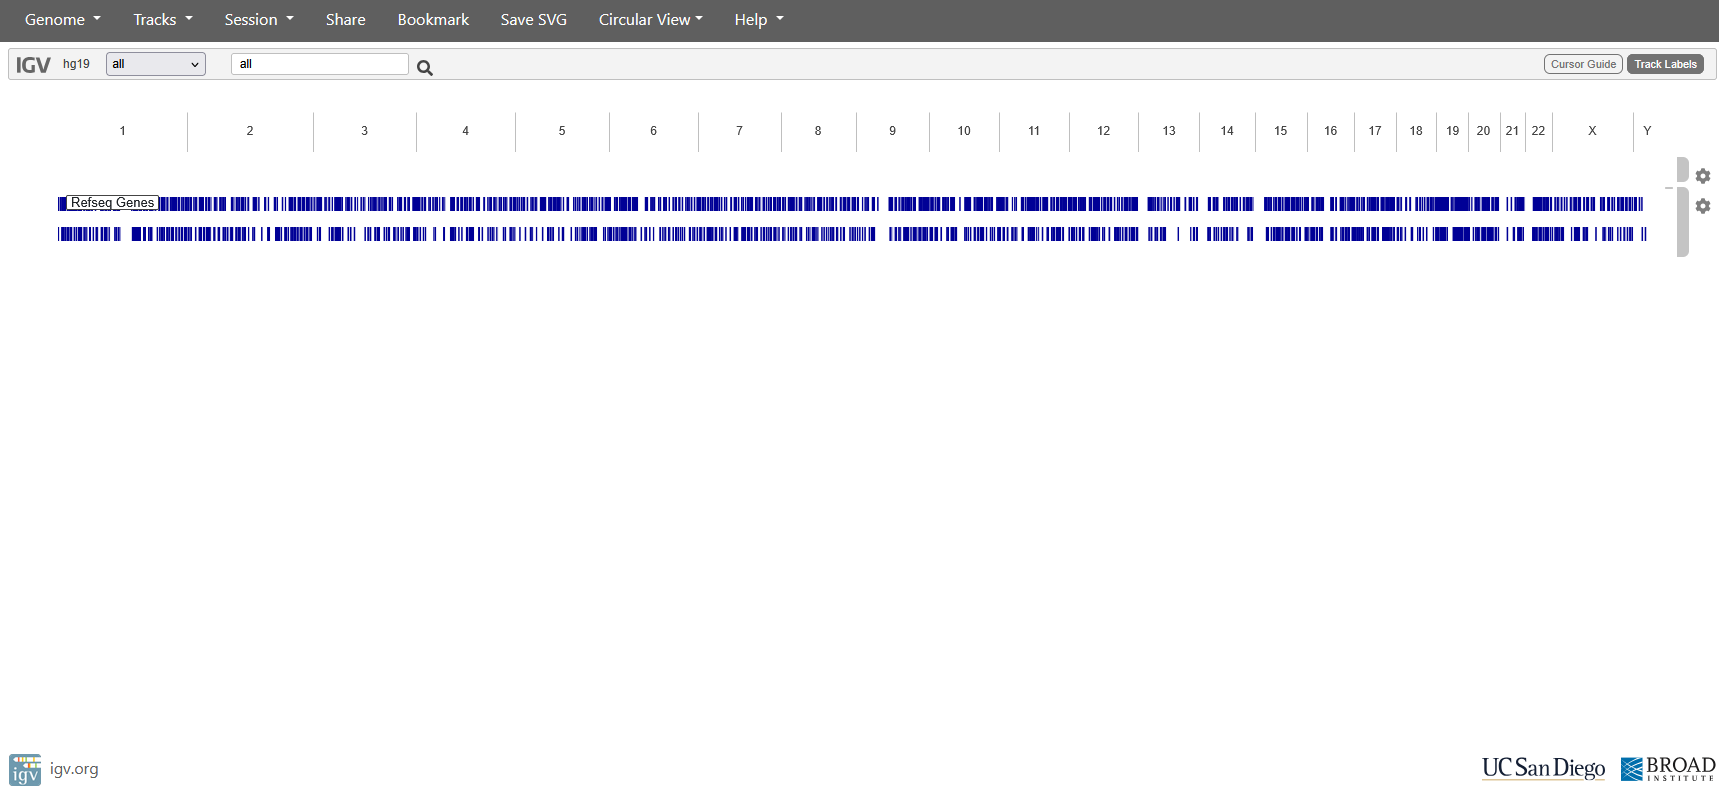
\includegraphics[keepaspectratio]{images/slide-03-image-1.png}}

The platinum WGS data we will be using have been aligned to version hg19
of the human reference genome, so we will need to first select the
GRCh37/hg19 reference sequence from the genome menu:

\pandocbounded{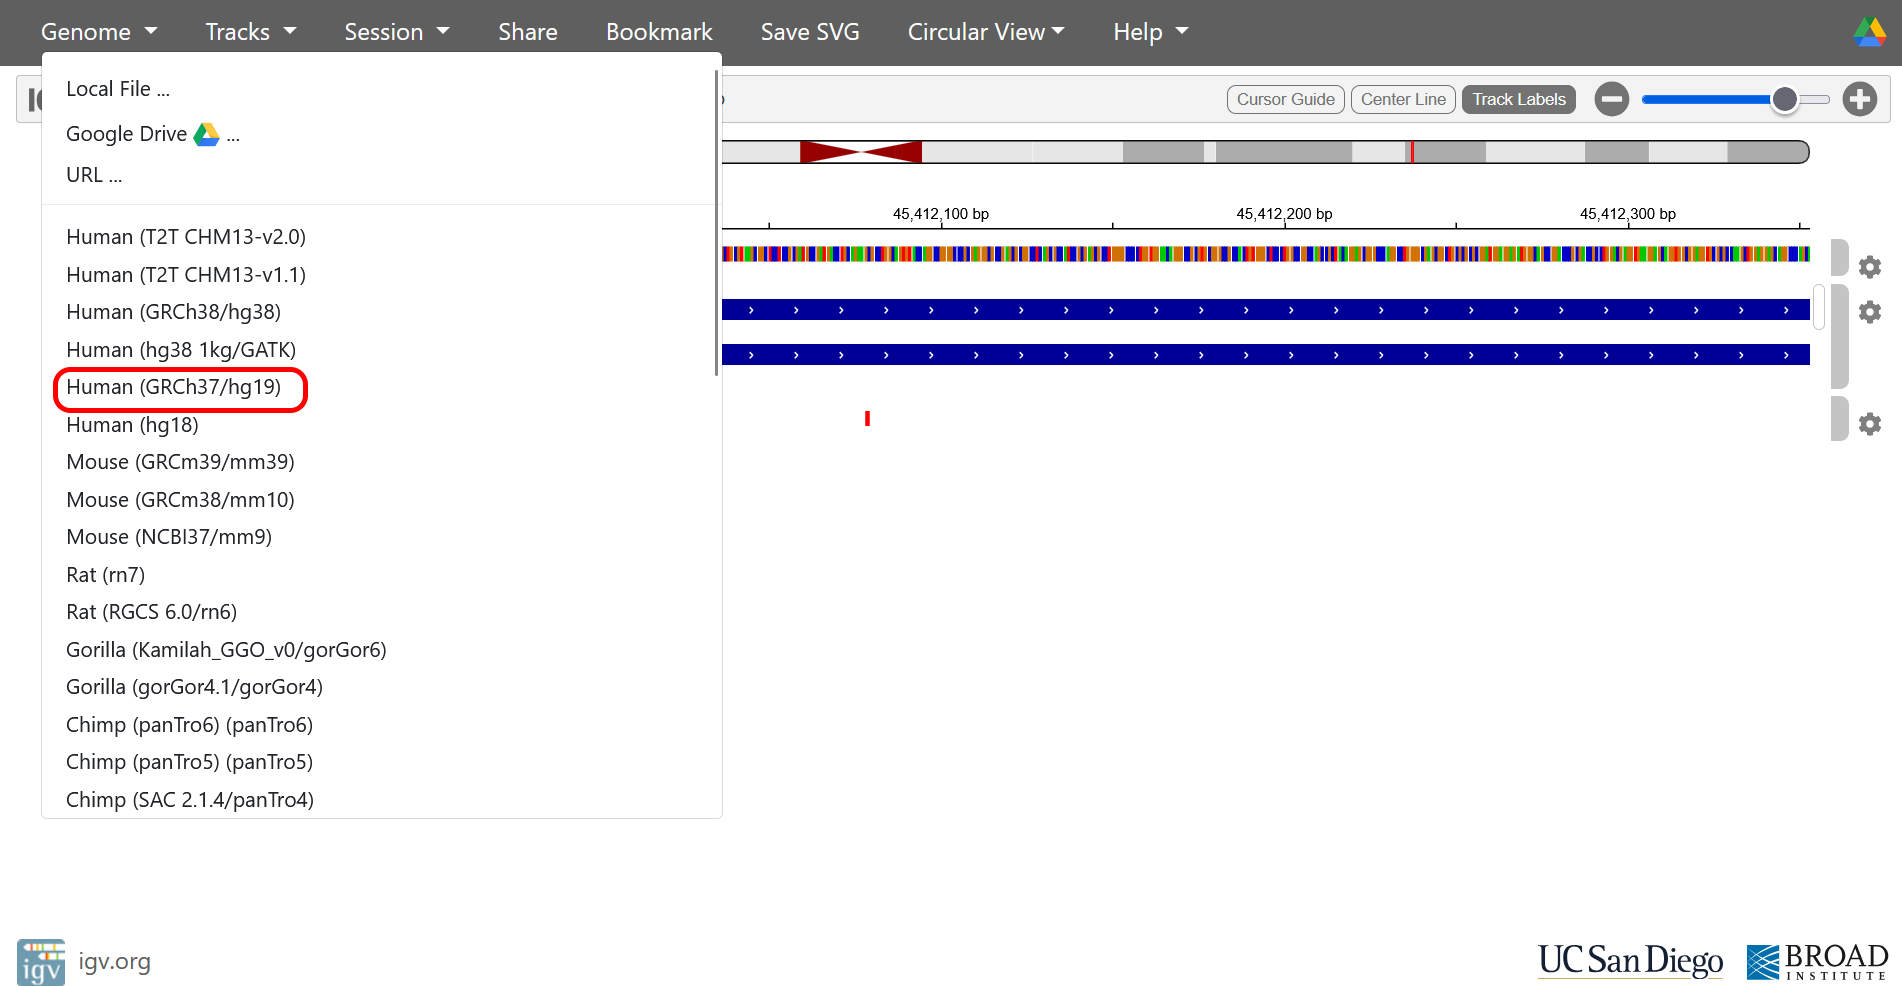
\includegraphics[keepaspectratio]{images/slide-genome-image-1.png}}

In order to interpret the sequence data, we are going to add some
additional ``Annotation'' ``Tracks'' to the IGV window:

\pandocbounded{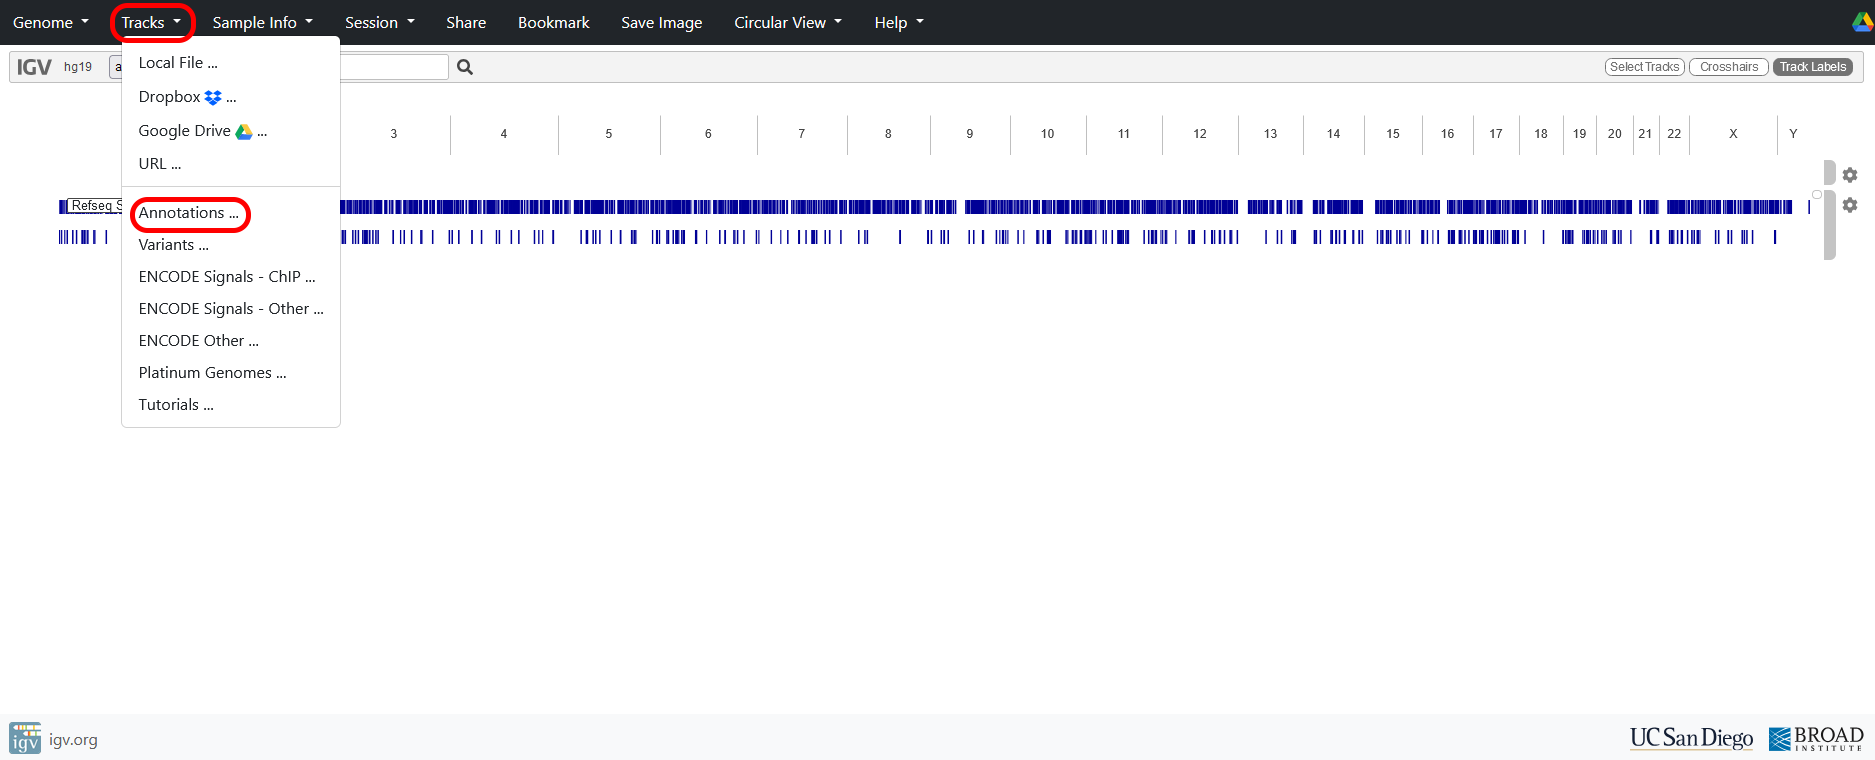
\includegraphics[keepaspectratio]{images/slide-04-image-1.png}}

Use Shift+Click to select the Repeat Masker and CpG Islands annotation
tracks (in addition to the Refseq Genes track which is a default track):

\pandocbounded{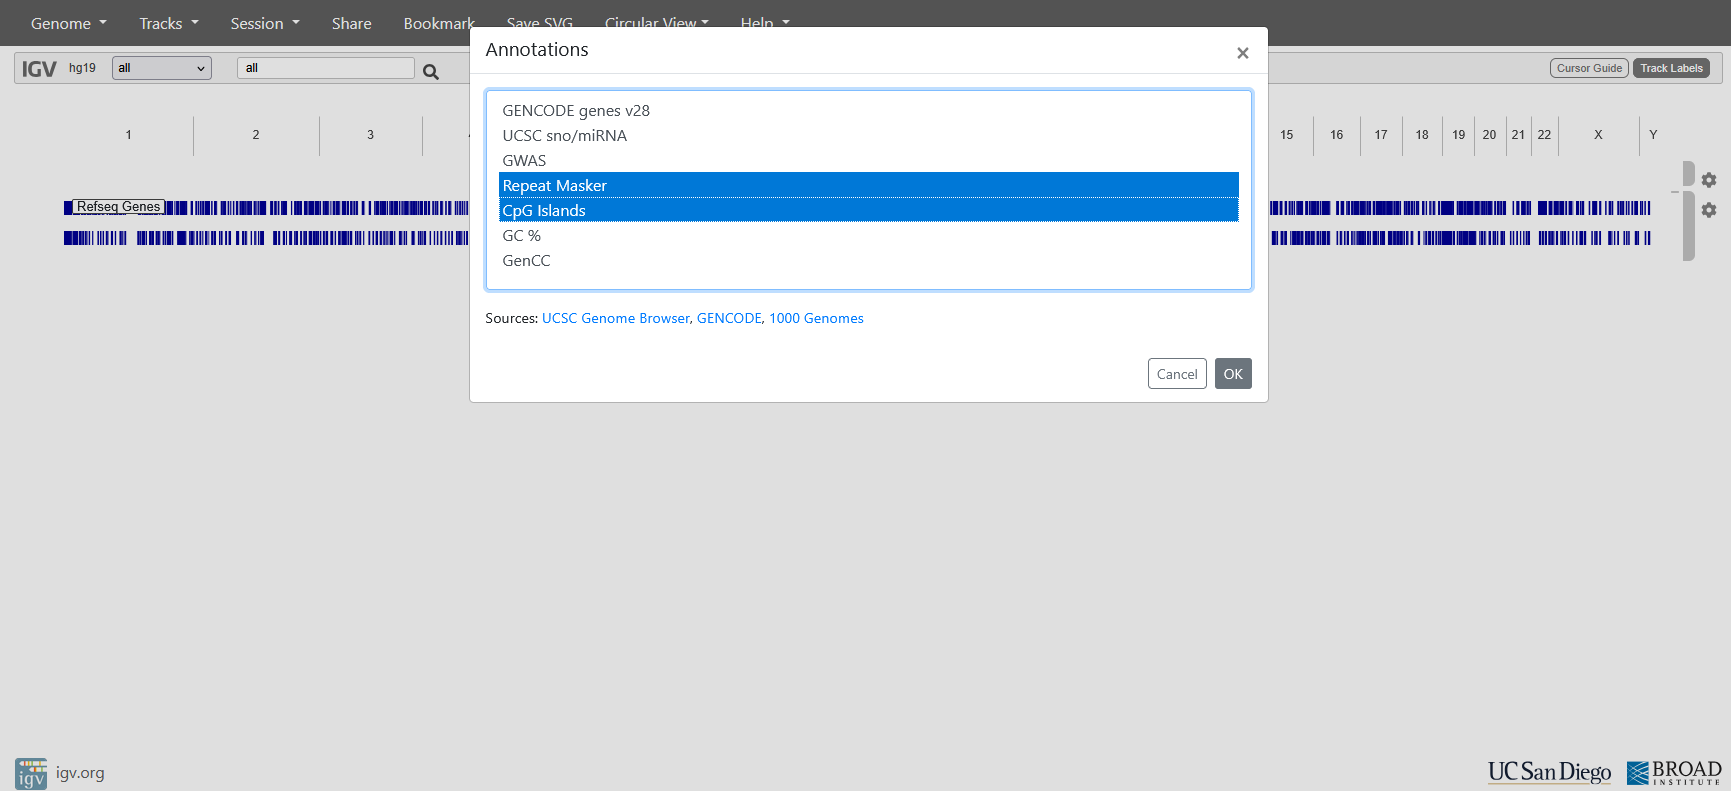
\includegraphics[keepaspectratio]{images/slide-05-image-1.png}}

We can also add some known ``variants'' as a track from the dbSNP
database (version 150):

\pandocbounded{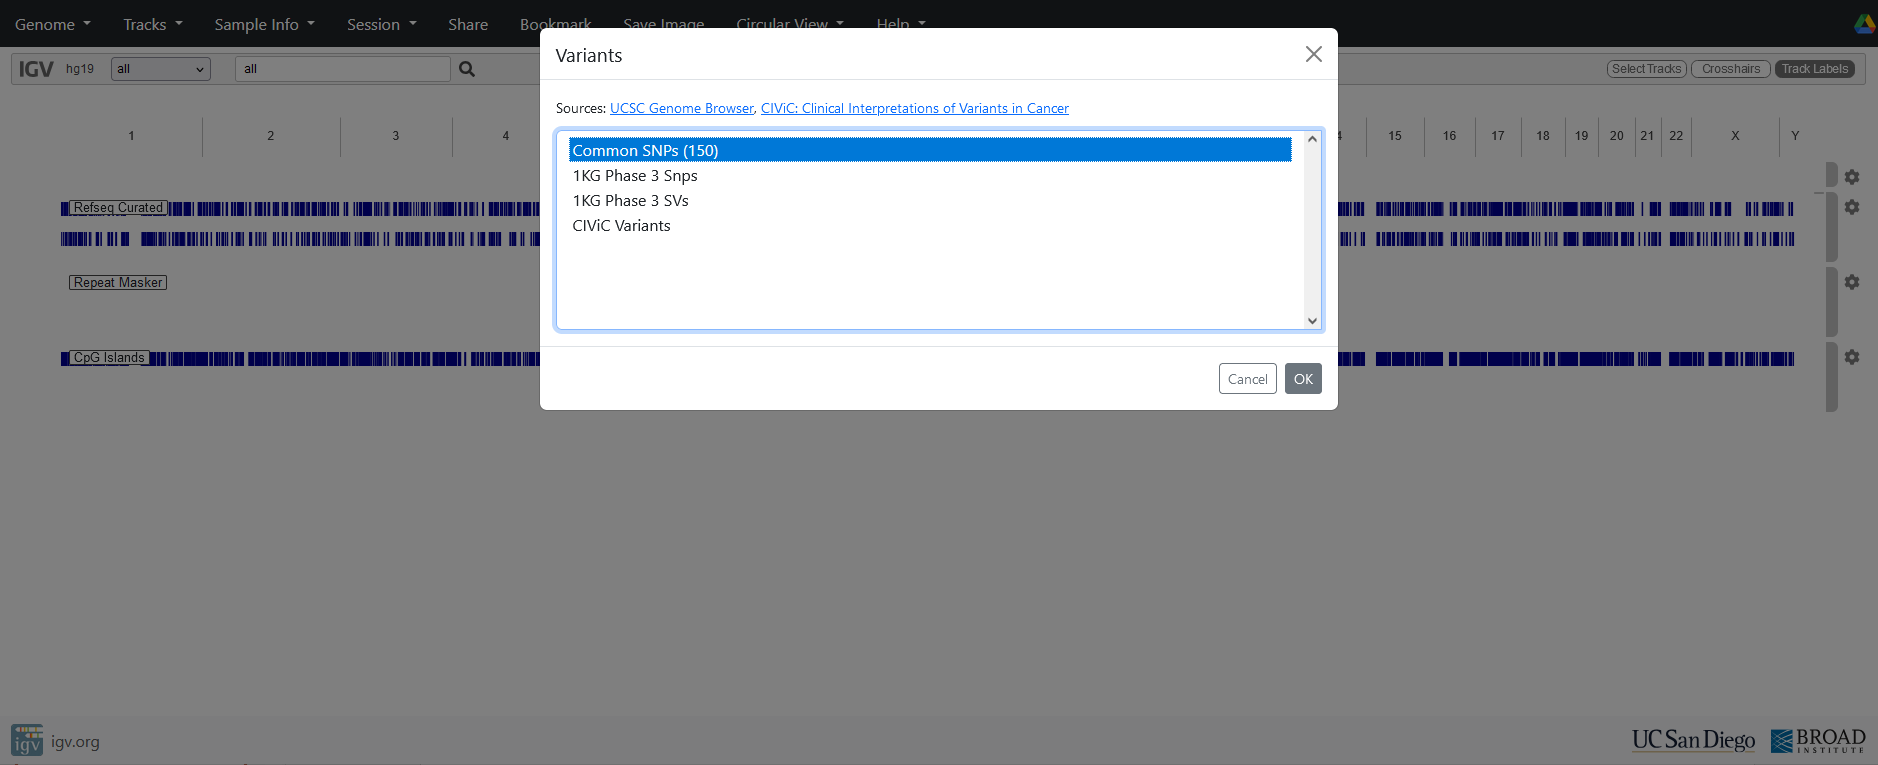
\includegraphics[keepaspectratio]{images/slide-06-image-1.png}}

Your window should now look something like this (you can use the grey
handle on the right to drag the Refseq Gene annotation back to the top):

\pandocbounded{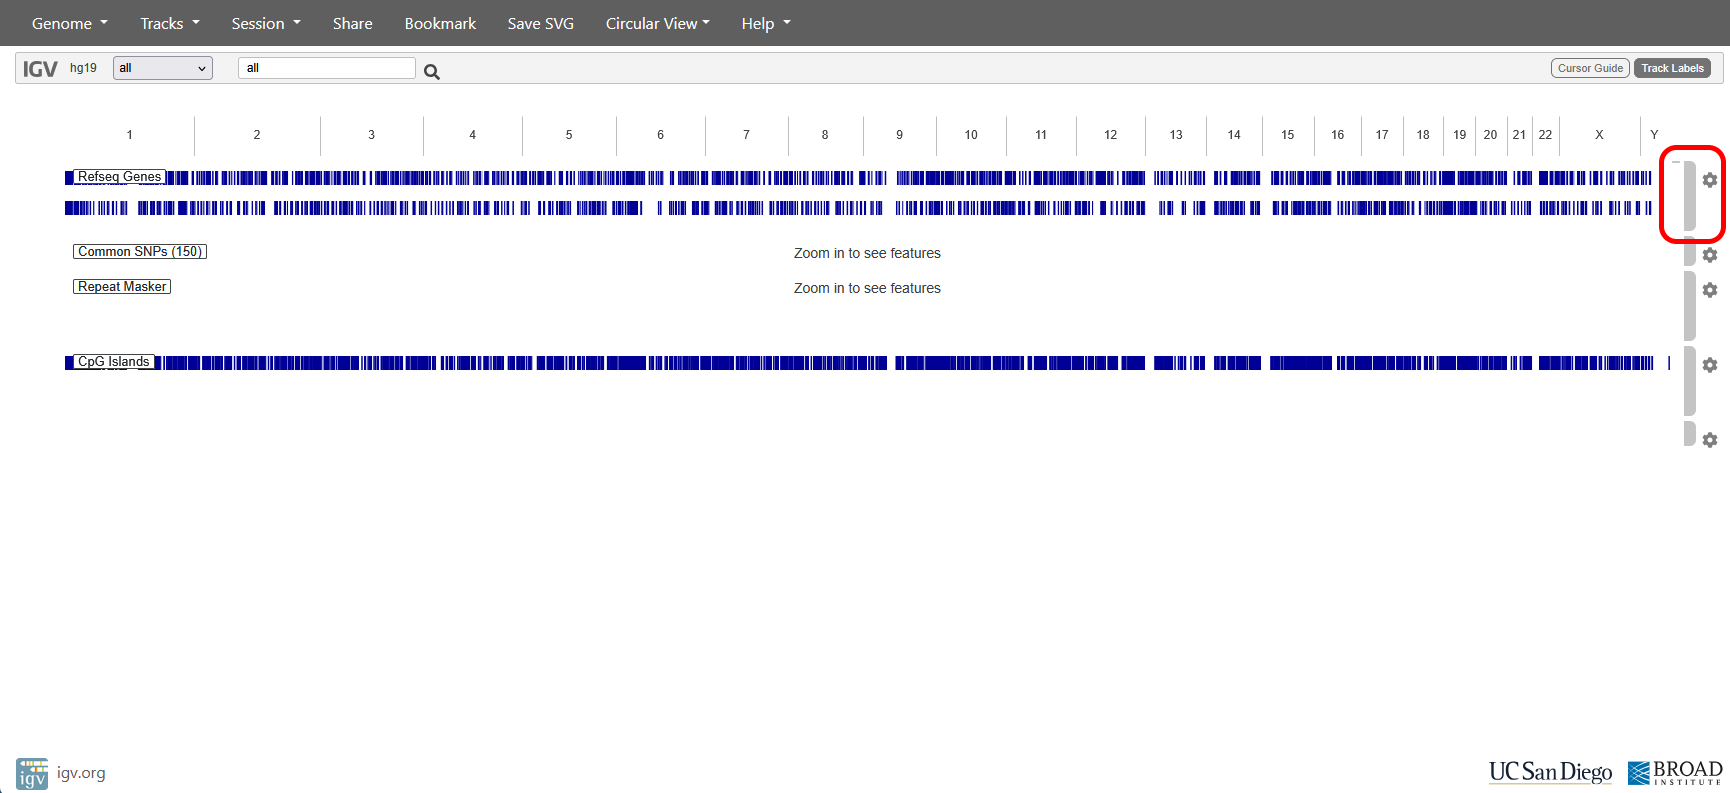
\includegraphics[keepaspectratio]{images/slide-07-image-1.png}}

\bookmarksetup{startatroot}

\chapter{Navigate the genome}\label{navigate-the-genome}

Before looking at any sequence data, get a feel for navigating around
the genome and remind yourself of some features of genome organisation.

To see more detail, we need to focus on a smaller region of the genome.
There are various ways to do this, including selecting a chromosome
either using the pull-down menu, or the chromosome buttons:

\pandocbounded{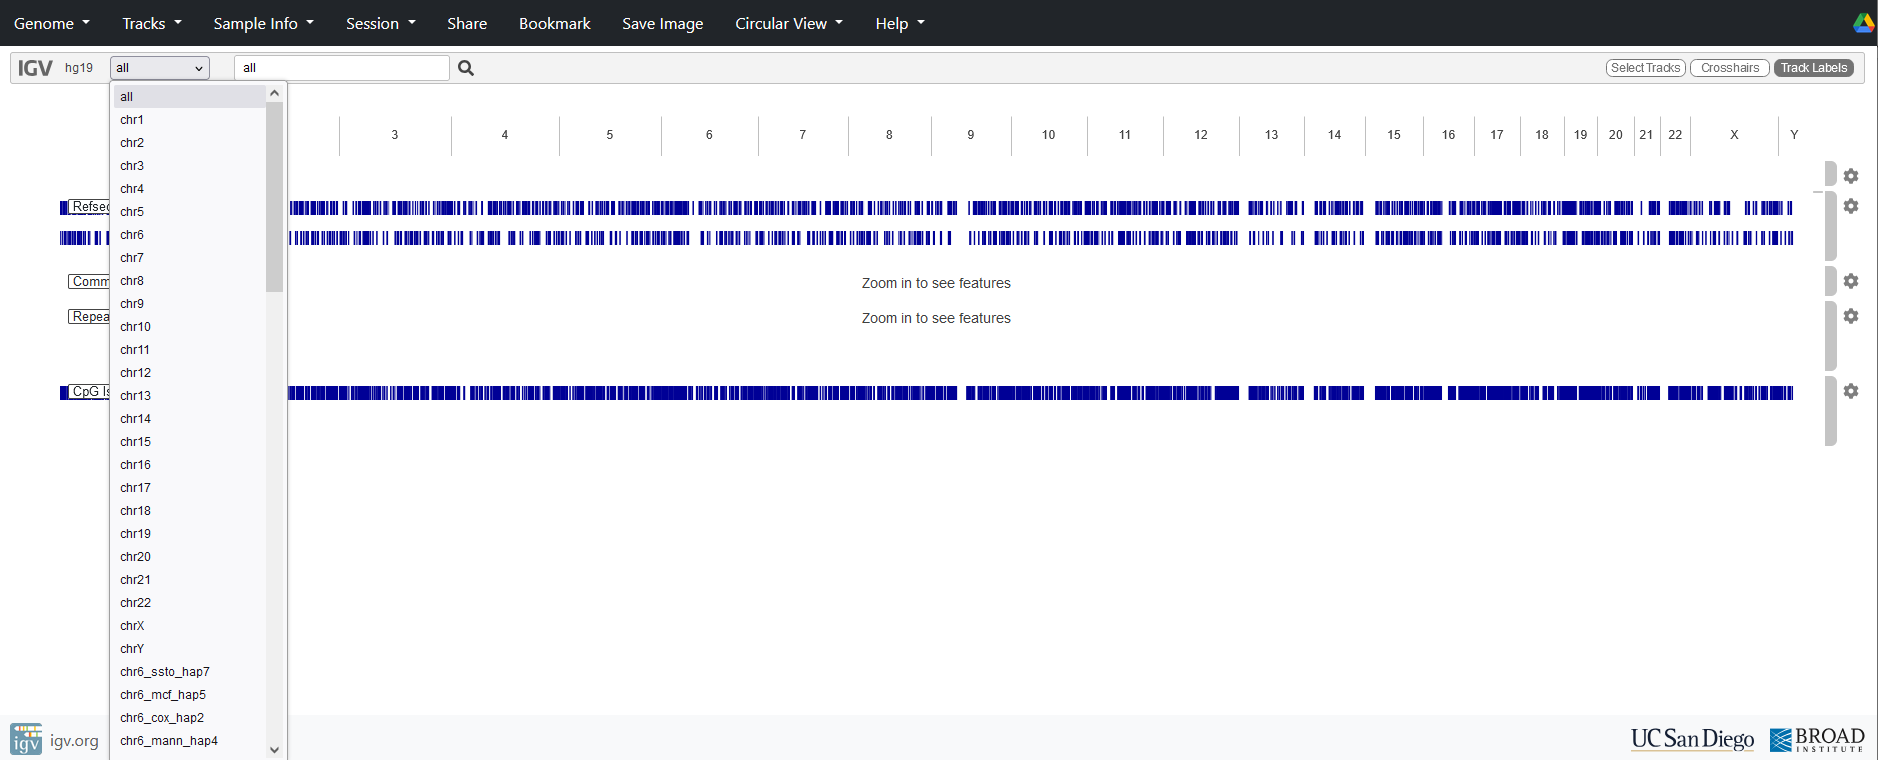
\includegraphics[keepaspectratio]{images/slide-08-image-1.png}}

Let's look at chromosome 8:

\pandocbounded{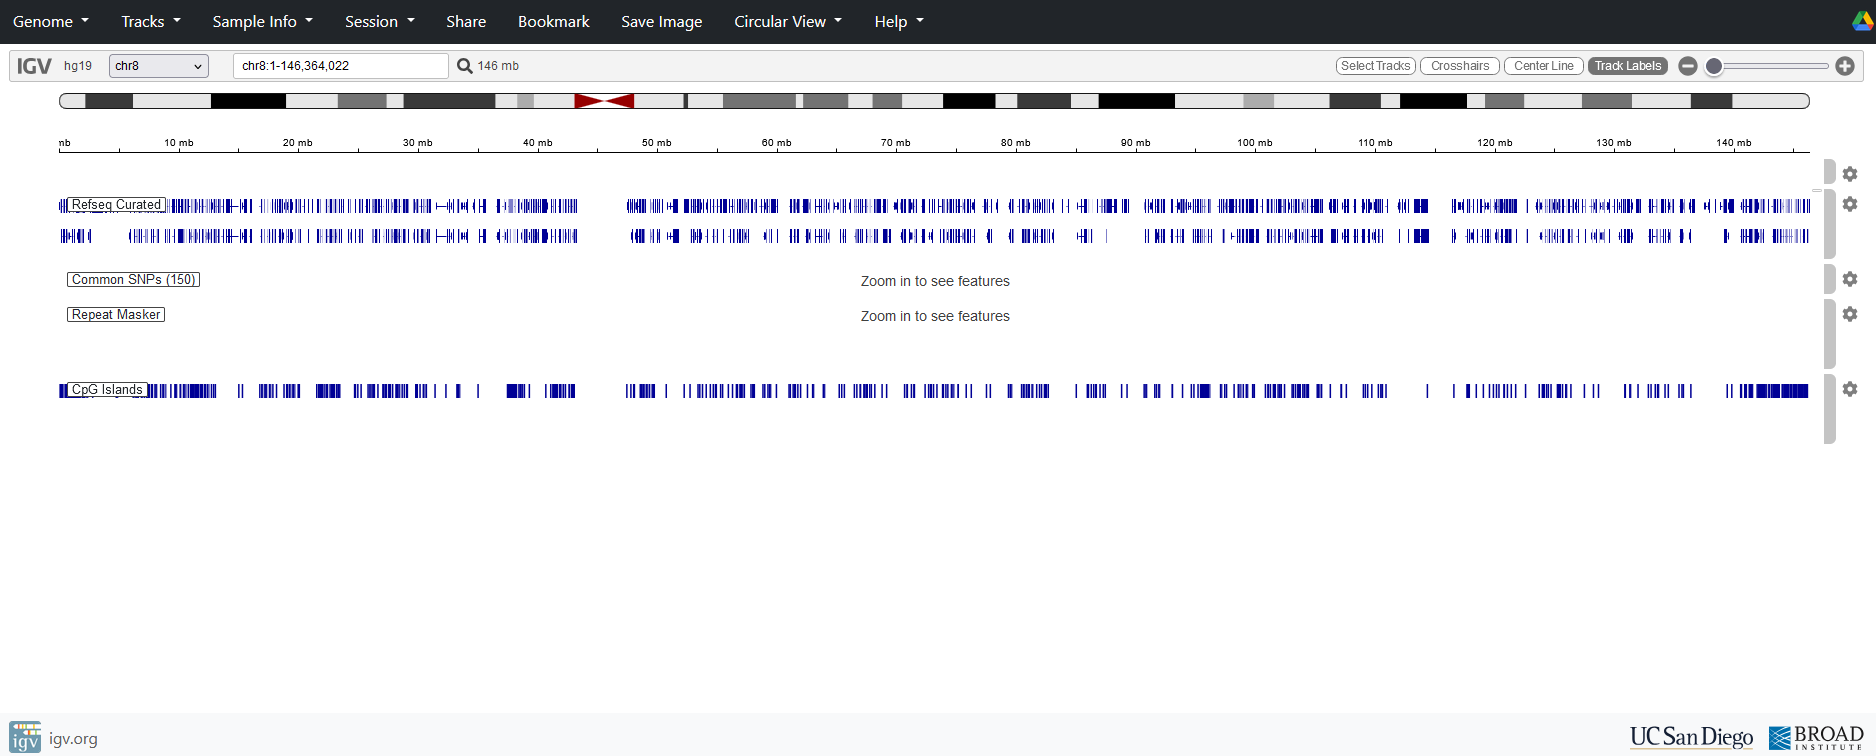
\includegraphics[keepaspectratio]{images/slide-09-image-1.png}}

At this level we can start to see some detail regarding the distribution
of known genes (A) and CpG islands (B).

\pandocbounded{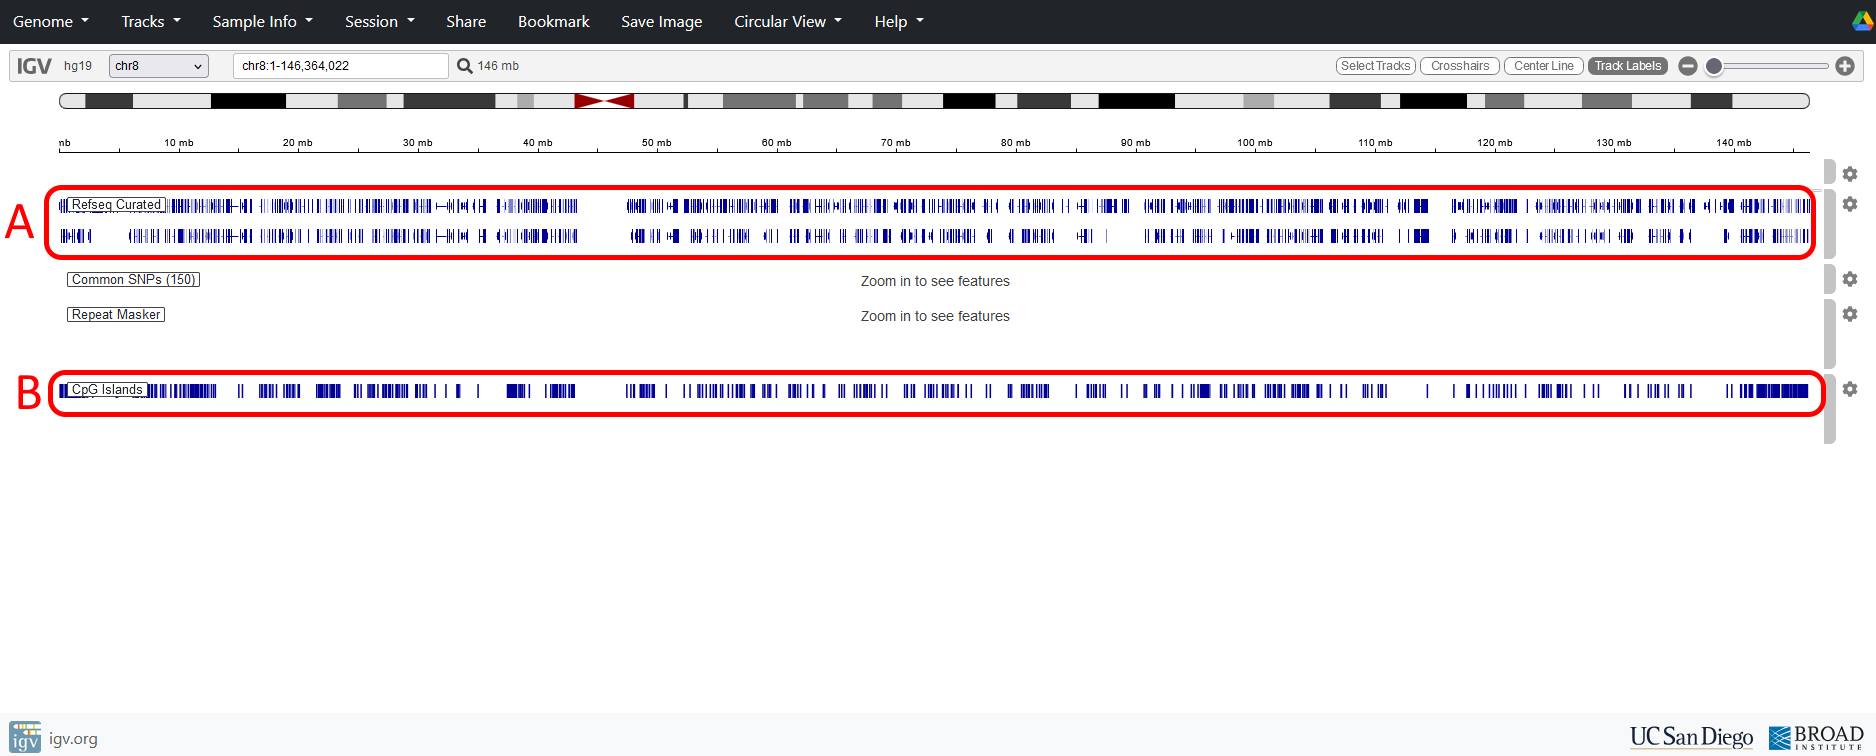
\includegraphics[keepaspectratio]{images/slide-10-image-1.png}}

We can zoom in further by either clicking and dragging on the scale (A),
typing in sequence coordinates (B), or using the zoom buttons (C).

\pandocbounded{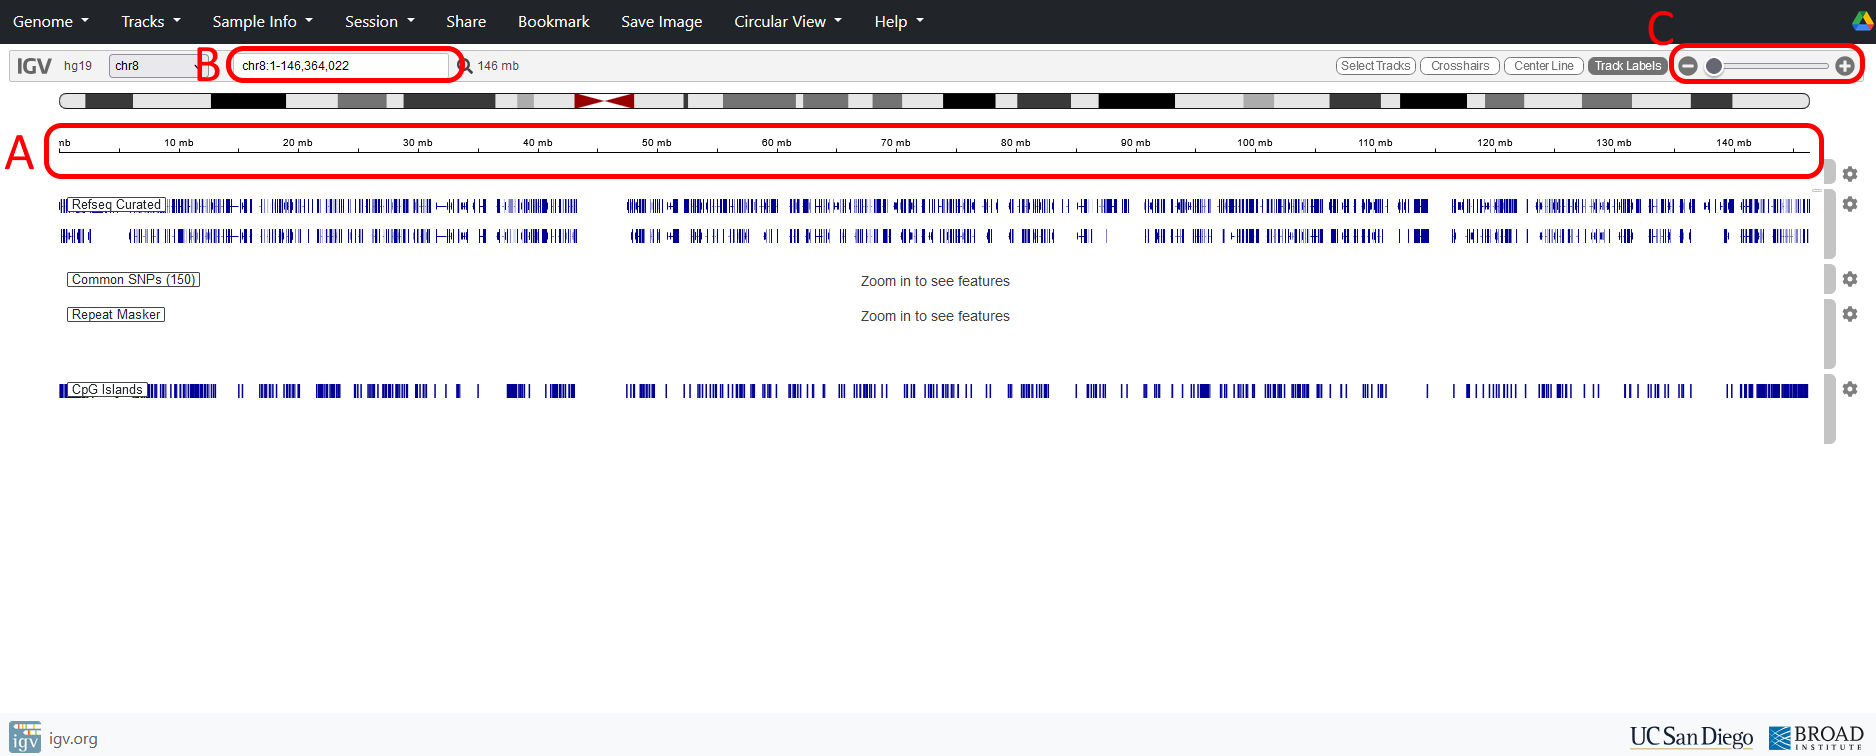
\includegraphics[keepaspectratio]{images/slide-11-image-1.png}}

Try pressing the + zoom button \textbf{five} times:

You should now start to see individual genes and CpG islands. Note how
genes and intergenic regions differ in size.

\pandocbounded{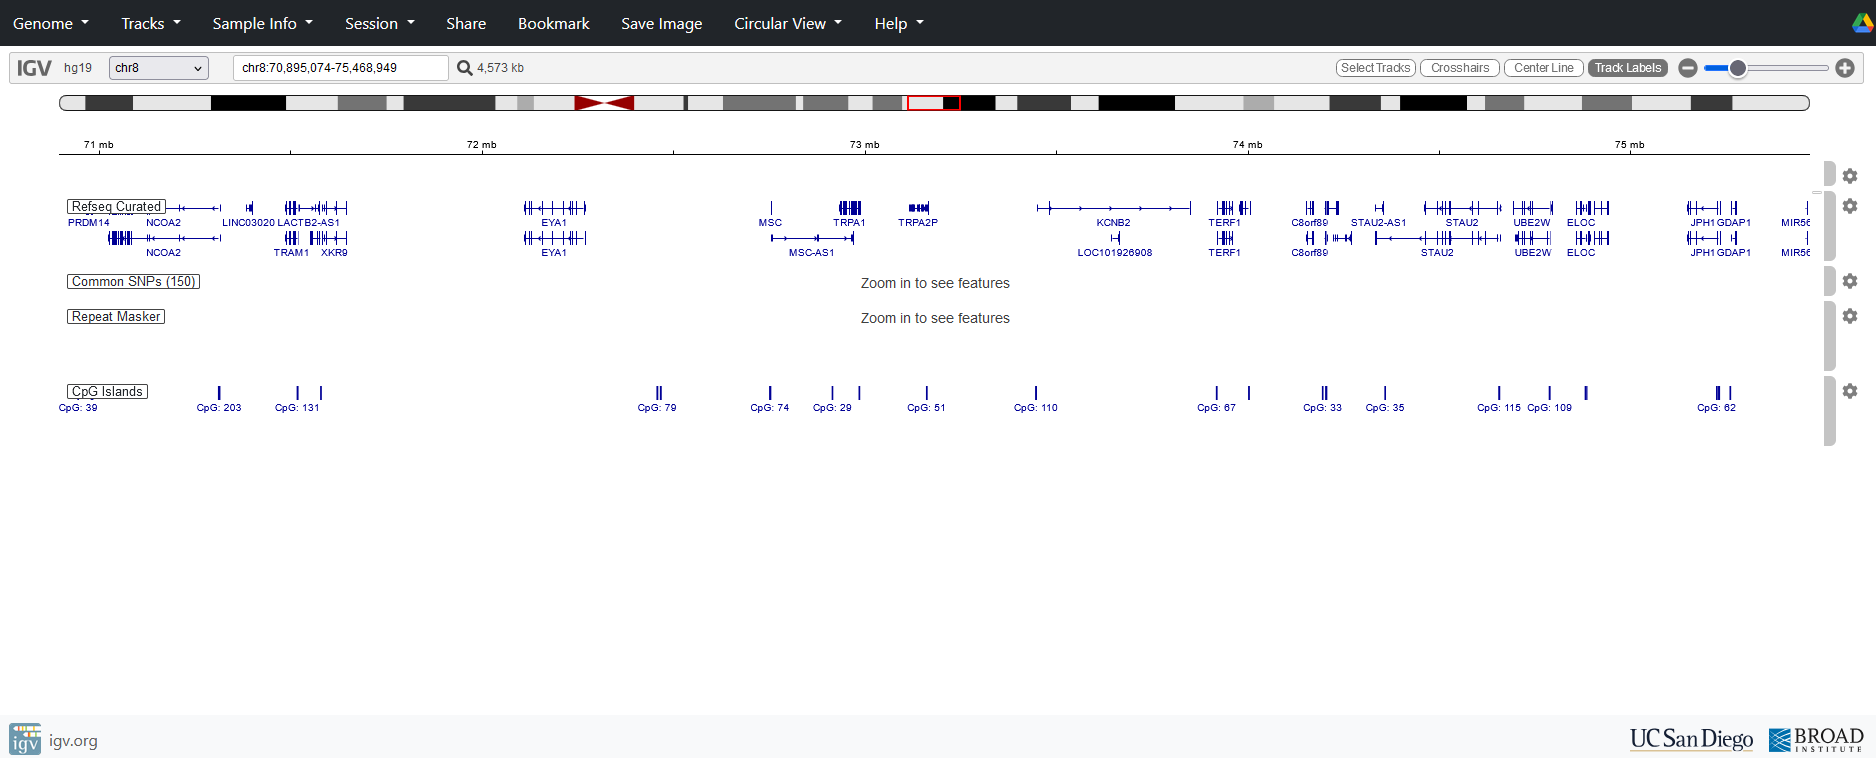
\includegraphics[keepaspectratio]{images/slide-12-image-1.png}}

You can press the ``Cursor Guide'' and ``Center Line'' buttons to help
with navigation.

\pandocbounded{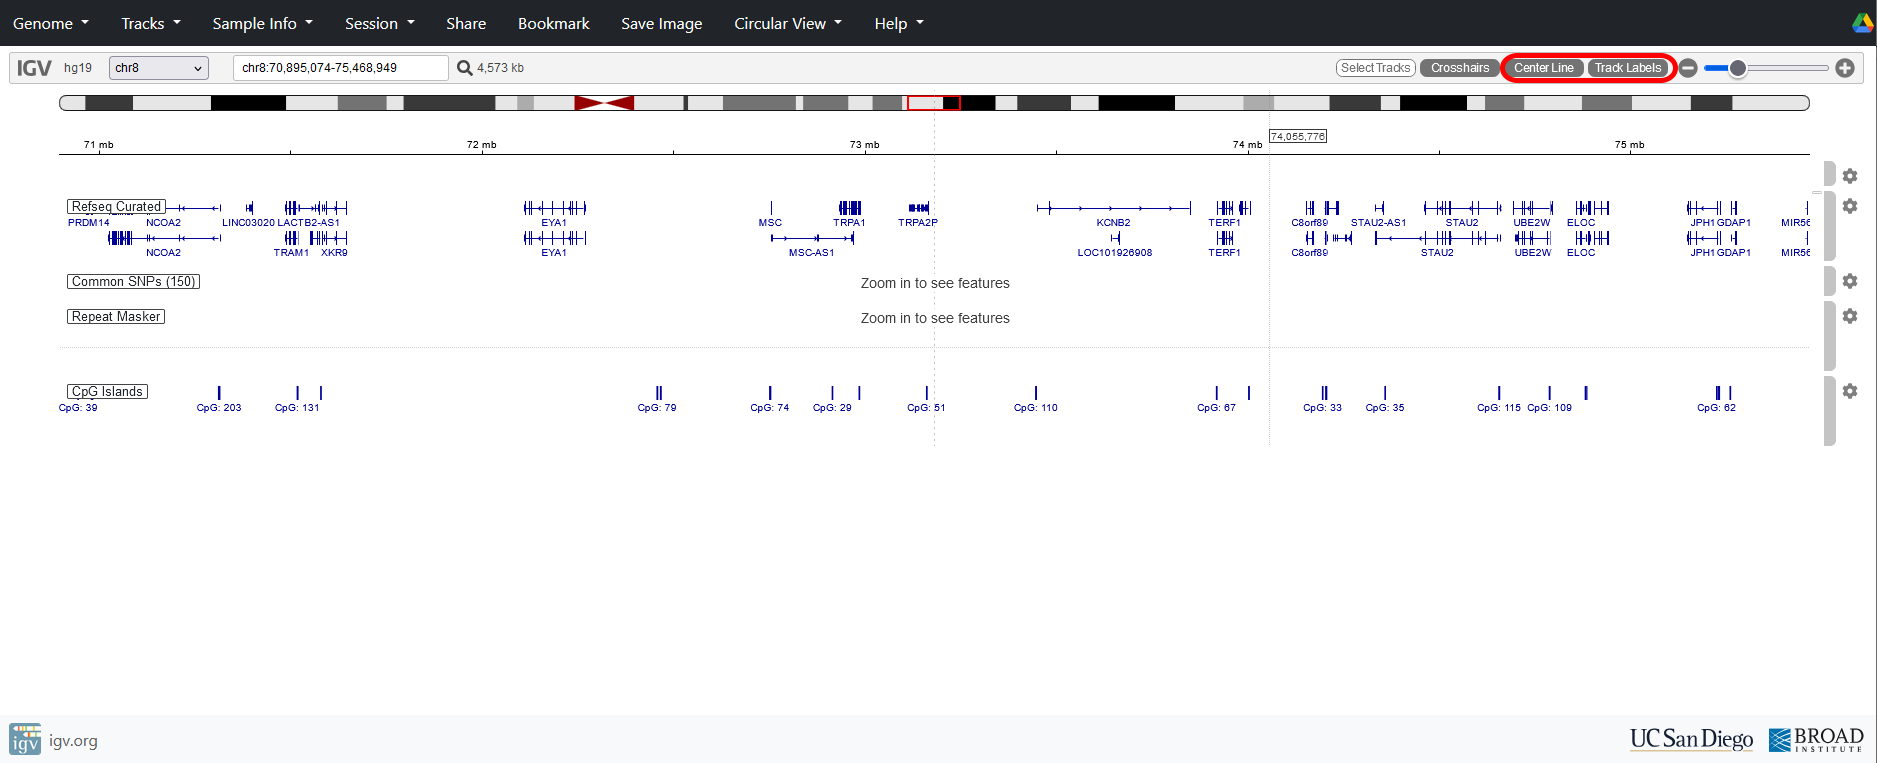
\includegraphics[keepaspectratio]{images/slide-13-image-1.png}}

\bookmarksetup{startatroot}

\chapter{\texorpdfstring{Interpret gene structure using
\emph{TERF1}}{Interpret gene structure using TERF1}}\label{interpret-gene-structure-using-terf1}

Once you have zoomed in a bit, you can now also navigate left and right
by clicking and dragging the cursor in the data window. Move the
\emph{TERF1} gene to the centre of the frame:

\pandocbounded{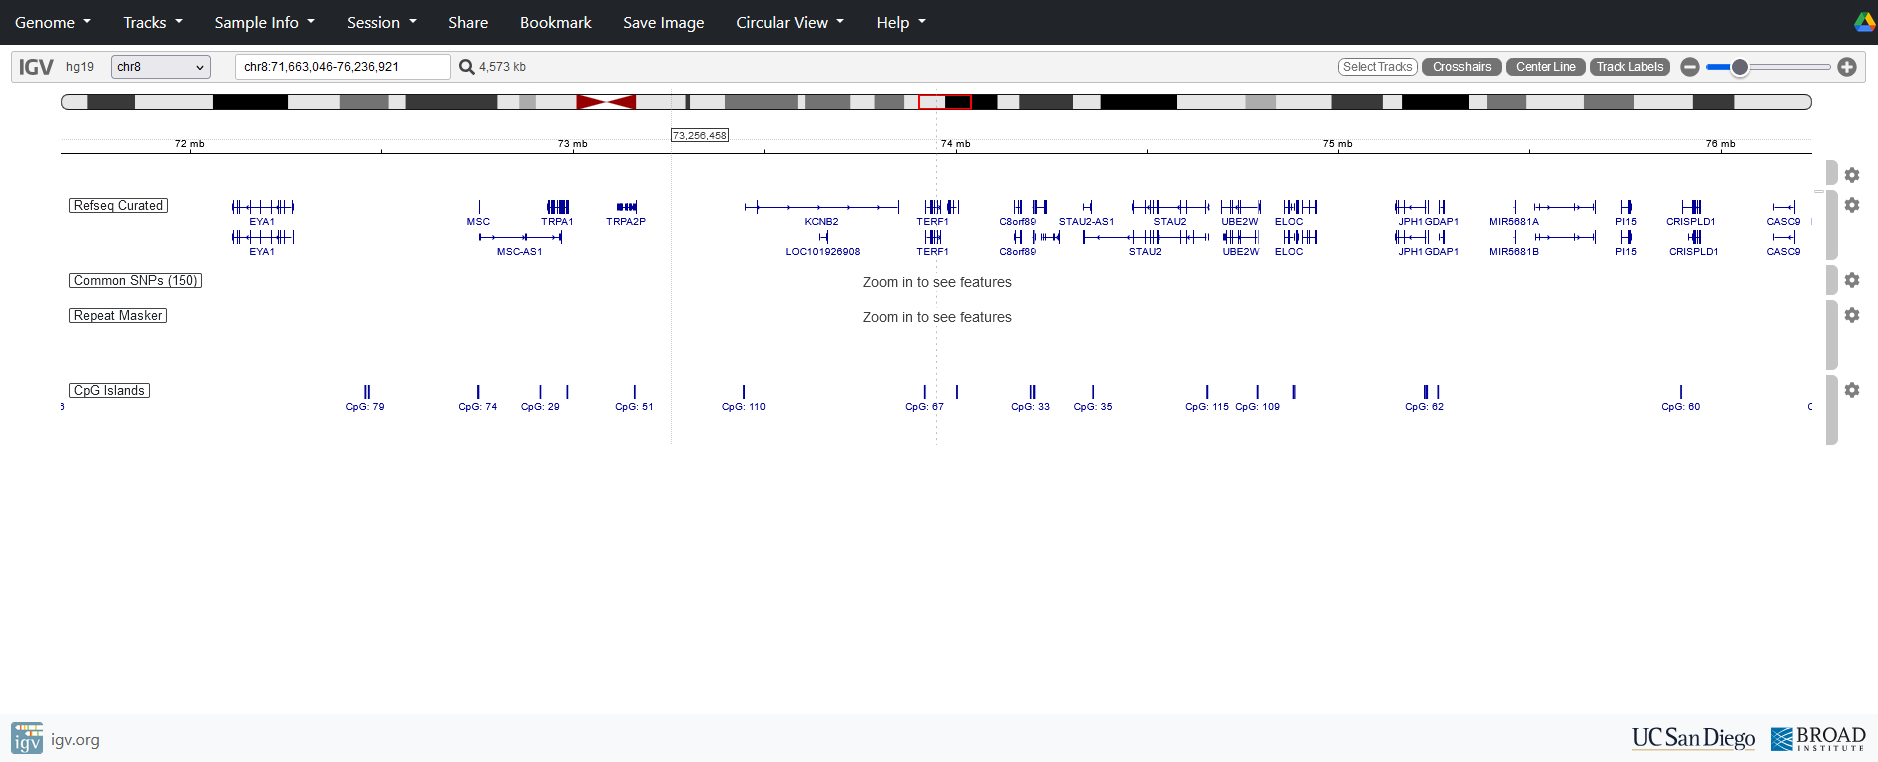
\includegraphics[keepaspectratio]{images/slide-14-image-1.png}}

\textbf{Exons} are indicated by the dark blue boxes with coding regions
taller than the non-coding parts of the exons. \textbf{Introns} are
indicated by the thin blue line, with the direction of transcription
indicated by small arrows (\textgreater).

Zoom in to see the structure of the \emph{TERF1} gene (there are two
primary transcripts for this gene):

\pandocbounded{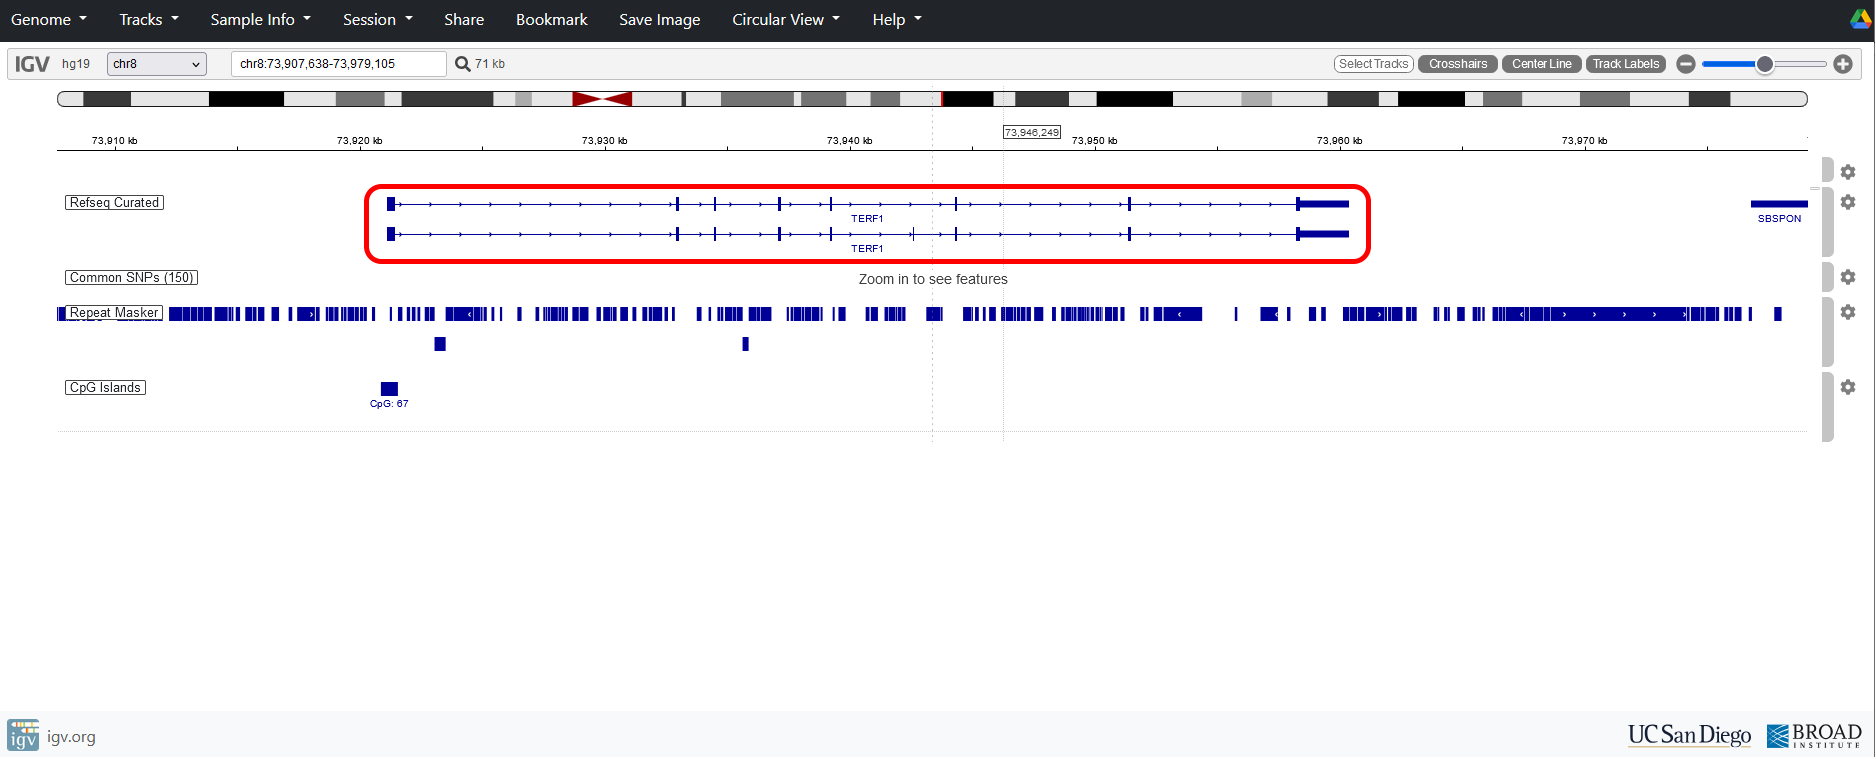
\includegraphics[keepaspectratio]{images/slide-15-image-1.png}}

\begin{tcolorbox}[enhanced jigsaw, arc=.35mm, bottomrule=.15mm, bottomtitle=1mm, breakable, colback=white, colbacktitle=quarto-callout-tip-color!10!white, colframe=quarto-callout-tip-color-frame, coltitle=black, left=2mm, leftrule=.75mm, opacityback=0, opacitybacktitle=0.6, rightrule=.15mm, title=\textcolor{quarto-callout-tip-color}{\faLightbulb}\hspace{0.5em}{Test your understanding}, titlerule=0mm, toprule=.15mm, toptitle=1mm]

\begin{itemize}
\tightlist
\item
  How many exons does the \emph{TERF1} gene have?
\end{itemize}

\end{tcolorbox}

\begin{tcolorbox}[enhanced jigsaw, arc=.35mm, bottomrule=.15mm, bottomtitle=1mm, breakable, colback=white, colbacktitle=quarto-callout-tip-color!10!white, colframe=quarto-callout-tip-color-frame, coltitle=black, left=2mm, leftrule=.75mm, opacityback=0, opacitybacktitle=0.6, rightrule=.15mm, title=\textcolor{quarto-callout-tip-color}{\faLightbulb}\hspace{0.5em}{Answer}, titlerule=0mm, toprule=.15mm, toptitle=1mm]

\emph{TERF1} has two primary transcripts, one with 9 exons (upper) and
one with 10 (lower).

\end{tcolorbox}

Move exon 1 of \emph{TERF1} to the centre and zoom in some more. You
should start to see the reference sequence appearing. You can also press
the cog on the track to turn on ``Three-frame translation'' to aid in
interpretation. This shows the amino acid sequences corresponding to the
three possible reading frames of the DNA sequence.

\pandocbounded{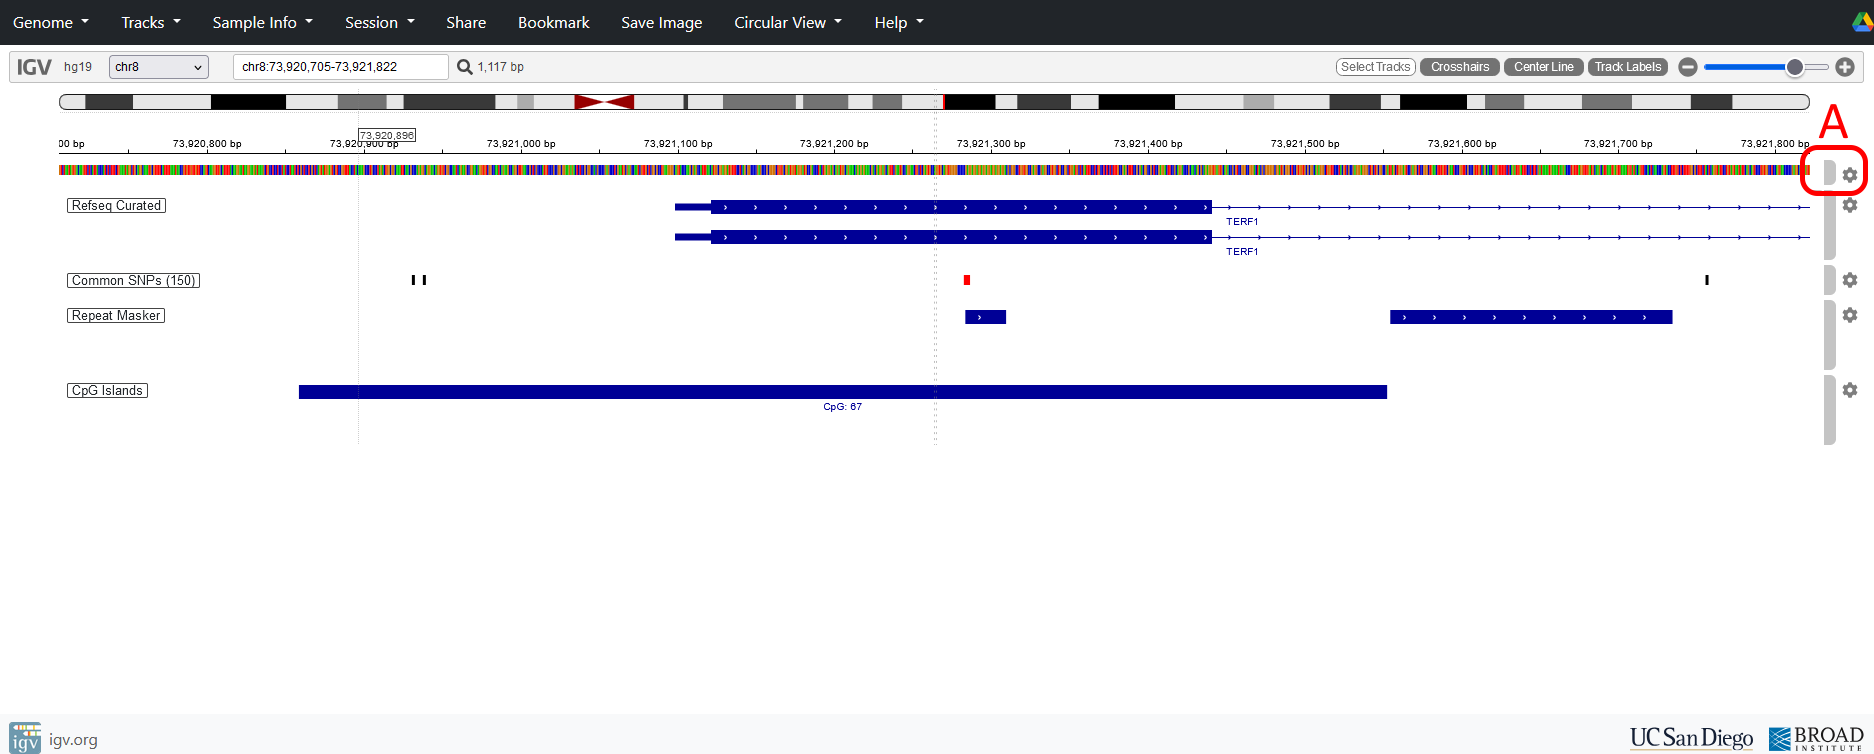
\includegraphics[keepaspectratio]{images/slide-16-image-1.png}}

\section{Add promoter-associated chromatin
data}\label{add-promoter-associated-chromatin-data}

We can add some additional information about the accessibility of DNA in
this region by adding an ENCODE Signal track containing ChIP-seq data
for H3K4me3 (trimethylation of lysine 4 on histone H3). This histone
variant is associated with open chromatin and marks active promoters in
the genome, typically appearing near transcription start sites (TSSs).

Add the ENCODE H3K4me3 track and select the `GM12878 H3K4me3 \textbar{}
Raw Signal \textbar{} Biorep 1' experiment near the bottom of the list
and press OK to add the track.

\pandocbounded{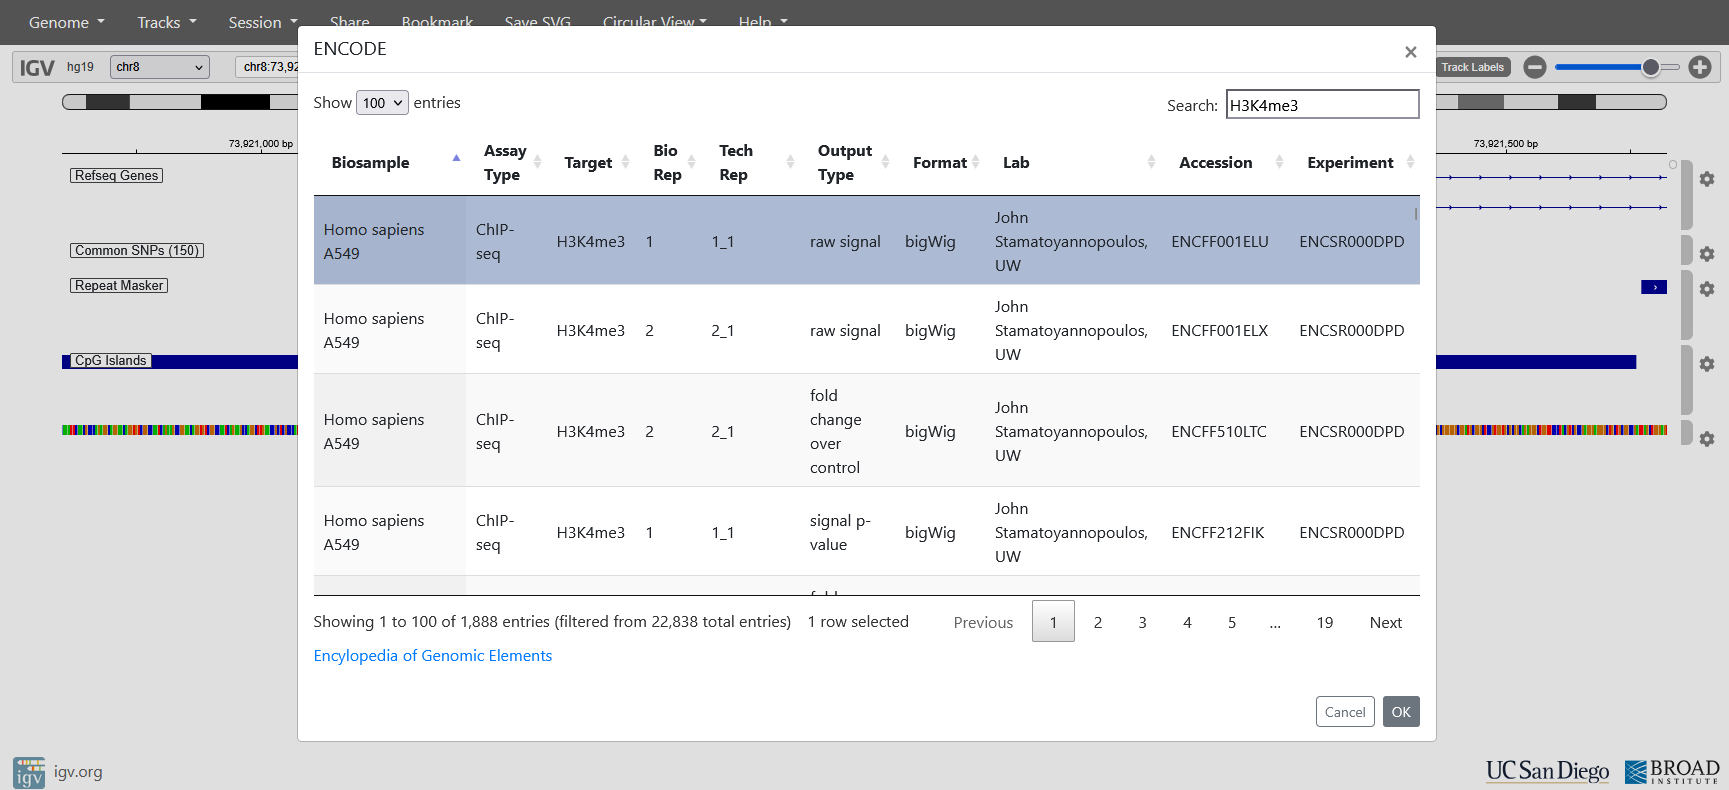
\includegraphics[keepaspectratio]{images/slide-17-image-1.png}}

\pandocbounded{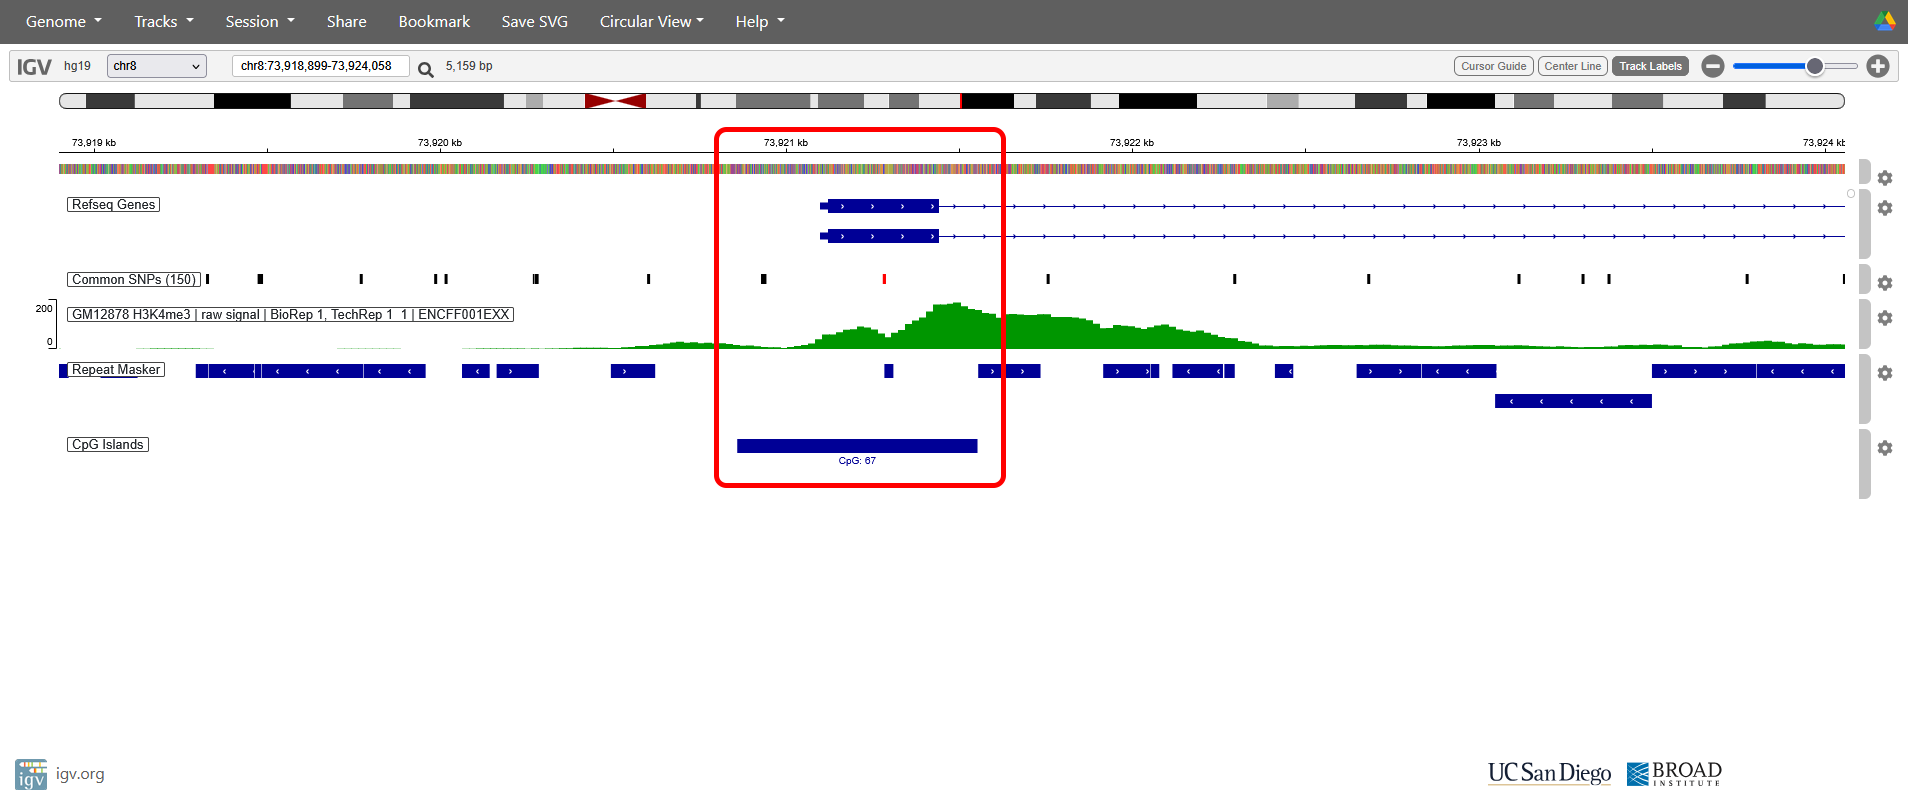
\includegraphics[keepaspectratio]{images/slide-18-image-1.png}}

\begin{tcolorbox}[enhanced jigsaw, arc=.35mm, bottomrule=.15mm, bottomtitle=1mm, breakable, colback=white, colbacktitle=quarto-callout-tip-color!10!white, colframe=quarto-callout-tip-color-frame, coltitle=black, left=2mm, leftrule=.75mm, opacityback=0, opacitybacktitle=0.6, rightrule=.15mm, title=\textcolor{quarto-callout-tip-color}{\faLightbulb}\hspace{0.5em}{Test your understanding}, titlerule=0mm, toprule=.15mm, toptitle=1mm]

\begin{itemize}
\tightlist
\item
  Is CpG island 67 positioned where you expect it to? (zooming in might
  help)
\item
  Why?
\item
  Which of the three reading frames do you think is correct for exon 1?
\item
  What is the name of the first repeated element in intron 1?
\end{itemize}

\end{tcolorbox}

\begin{tcolorbox}[enhanced jigsaw, arc=.35mm, bottomrule=.15mm, bottomtitle=1mm, breakable, colback=white, colbacktitle=quarto-callout-tip-color!10!white, colframe=quarto-callout-tip-color-frame, coltitle=black, left=2mm, leftrule=.75mm, opacityback=0, opacitybacktitle=0.6, rightrule=.15mm, title=\textcolor{quarto-callout-tip-color}{\faLightbulb}\hspace{0.5em}{Answer}, titlerule=0mm, toprule=.15mm, toptitle=1mm]

\begin{itemize}
\tightlist
\item
  Yes, CpG island 67 spans a promoter region in exon 1 and associates
  with H3K4me3 ChIP-seq data (typically found at TSSs and in open
  chromatin).
\item
  The correct frame starts with an ATG and has no STOP codons within
  exon 1. It will depend on your particular instance of IGV.
\item
  The first repeated element is a MIRb element and there are some
  additional Alu, LINE and MIR elements, and simple sequence repeats,
  further down. Note that \textasciitilde80\% of intron 1 sequence is
  some sort of repeat.
\end{itemize}

\end{tcolorbox}

\section{Examine splice junctions}\label{examine-splice-junctions}

Splice junctions mark the boundaries between exons and introns and are
critical for the accurate removal of intronic sequence during RNA
splicing. Adjust the view to examine the end of the first exon.

\begin{tcolorbox}[enhanced jigsaw, arc=.35mm, bottomrule=.15mm, bottomtitle=1mm, breakable, colback=white, colbacktitle=quarto-callout-warning-color!10!white, colframe=quarto-callout-warning-color-frame, coltitle=black, left=2mm, leftrule=.75mm, opacityback=0, opacitybacktitle=0.6, rightrule=.15mm, title=\textcolor{quarto-callout-warning-color}{\faExclamationTriangle}\hspace{0.5em}{Warning}, titlerule=0mm, toprule=.15mm, toptitle=1mm]

Be careful - the vertical order of the reading frames sometimes jumps
about as you zoom in and out.

\end{tcolorbox}

\pandocbounded{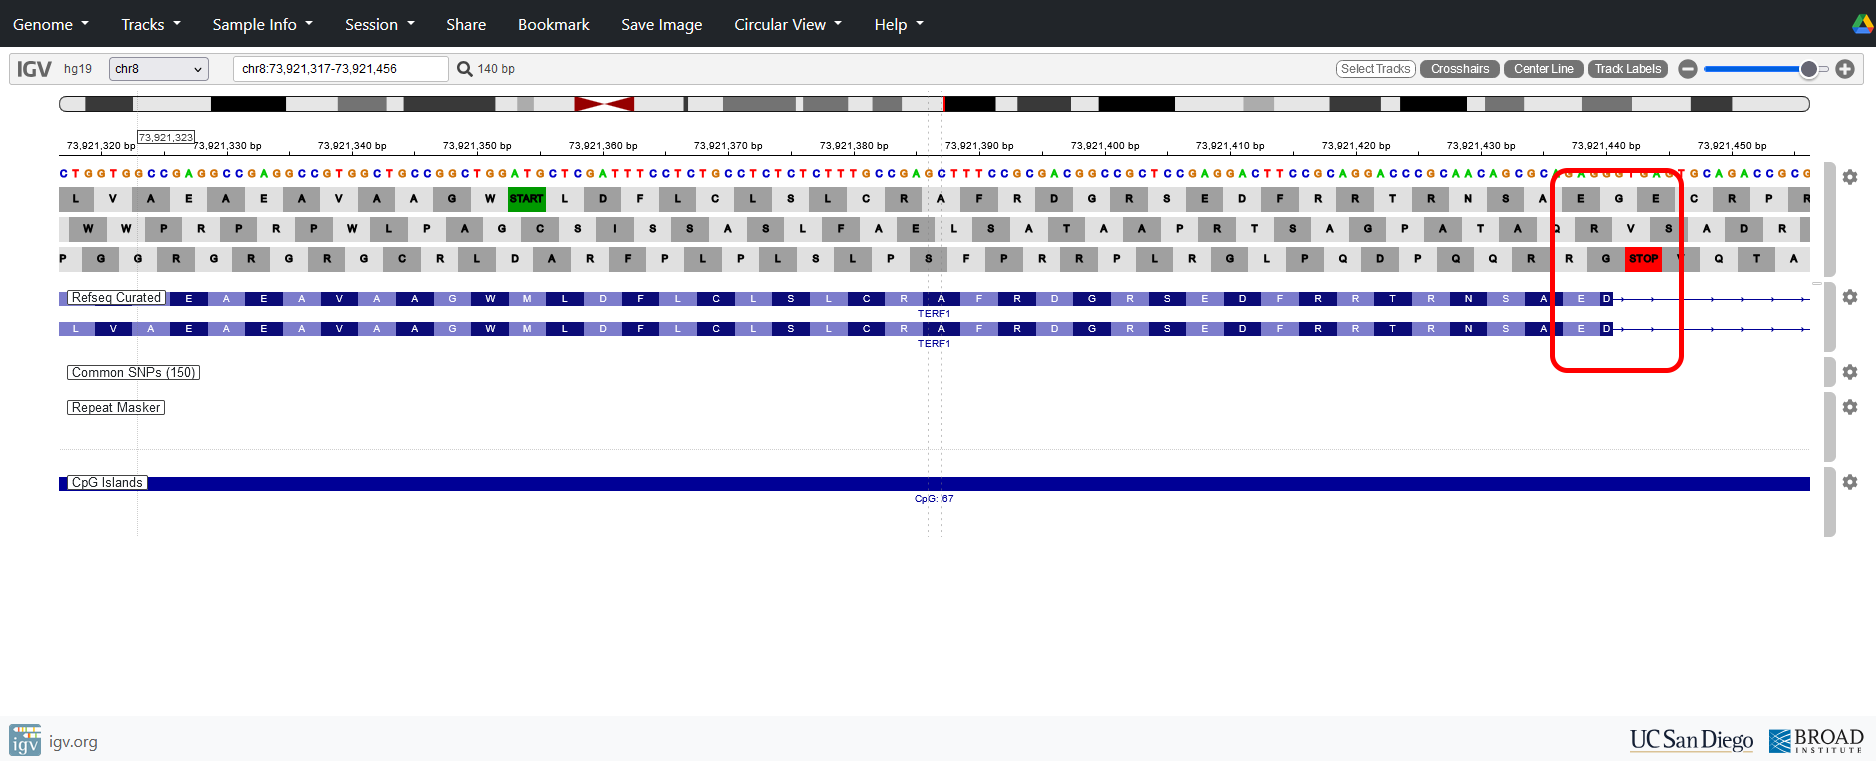
\includegraphics[keepaspectratio]{images/slide-19-image-1.png}}

\begin{tcolorbox}[enhanced jigsaw, arc=.35mm, bottomrule=.15mm, bottomtitle=1mm, breakable, colback=white, colbacktitle=quarto-callout-tip-color!10!white, colframe=quarto-callout-tip-color-frame, coltitle=black, left=2mm, leftrule=.75mm, opacityback=0, opacitybacktitle=0.6, rightrule=.15mm, title=\textcolor{quarto-callout-tip-color}{\faLightbulb}\hspace{0.5em}{Test your understanding}, titlerule=0mm, toprule=.15mm, toptitle=1mm]

\begin{itemize}
\tightlist
\item
  What is the sequence of the last codon of exon 1?
\item
  What is the sequence of the first two bases of the intron?
\item
  Why is this important?
\end{itemize}

\end{tcolorbox}

\begin{tcolorbox}[enhanced jigsaw, arc=.35mm, bottomrule=.15mm, bottomtitle=1mm, breakable, colback=white, colbacktitle=quarto-callout-tip-color!10!white, colframe=quarto-callout-tip-color-frame, coltitle=black, left=2mm, leftrule=.75mm, opacityback=0, opacitybacktitle=0.6, rightrule=.15mm, title=\textcolor{quarto-callout-tip-color}{\faLightbulb}\hspace{0.5em}{Answer}, titlerule=0mm, toprule=.15mm, toptitle=1mm]

\begin{itemize}
\tightlist
\item
  It will depend on your IGV instance but in this image it is the bottom
  frame as this matches the start codon at the beginning of the
  transcript, so the last codon is \textbf{G--}
\item
  The first two bases of the intron are GT
\item
  This is the consensus splice donor site
\end{itemize}

\end{tcolorbox}

Adjust the view to examine the end of the first intron and the beginning
of the second exon.

\pandocbounded{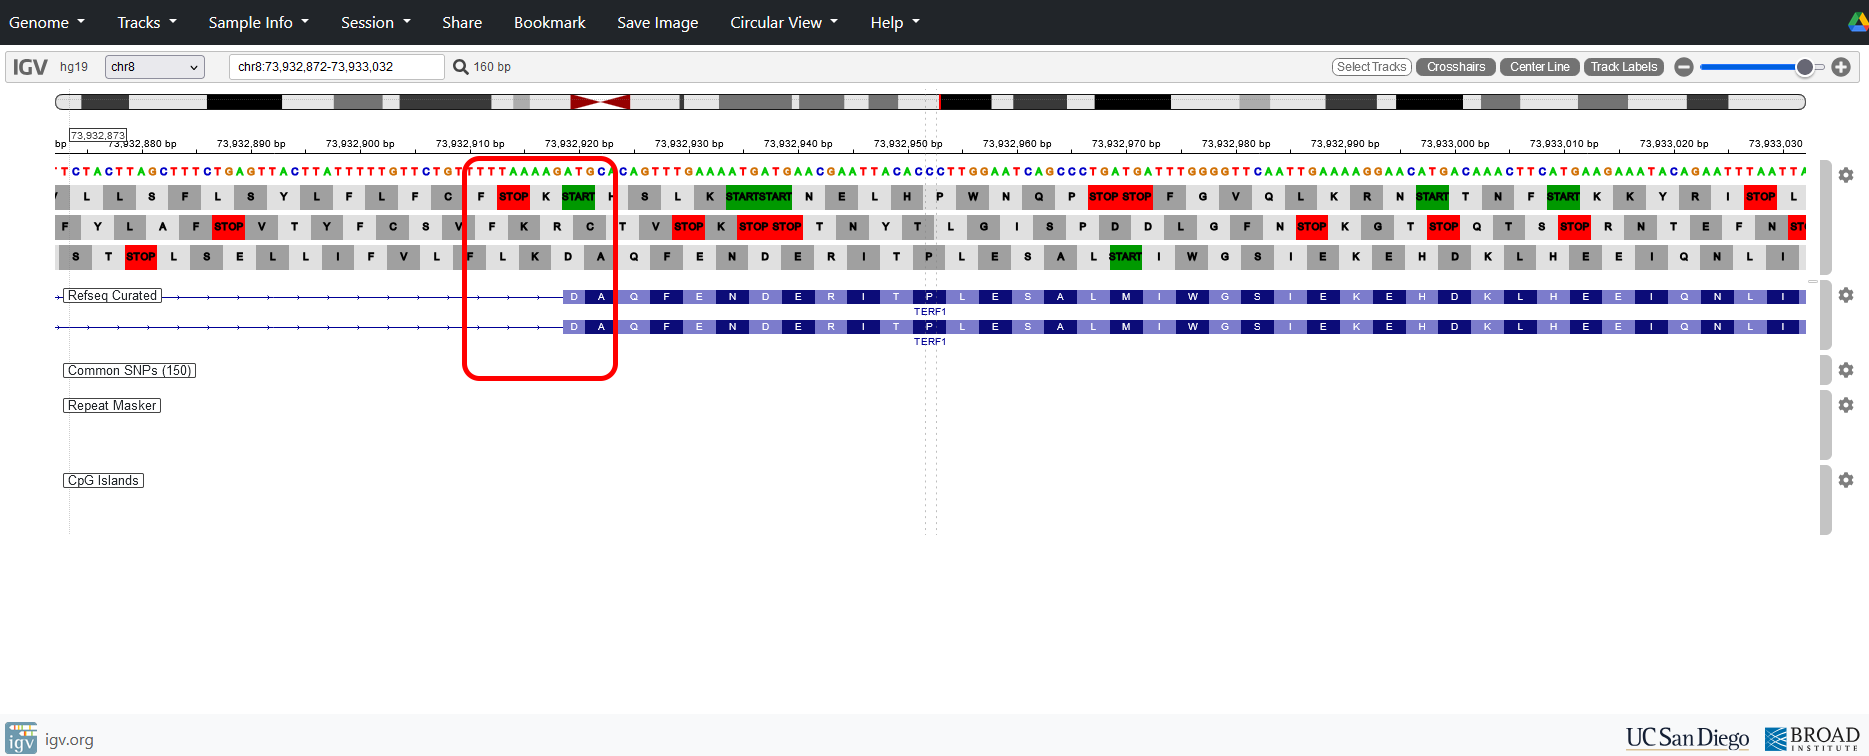
\includegraphics[keepaspectratio]{images/slide-20-image-1.png}}

\begin{tcolorbox}[enhanced jigsaw, arc=.35mm, bottomrule=.15mm, bottomtitle=1mm, breakable, colback=white, colbacktitle=quarto-callout-tip-color!10!white, colframe=quarto-callout-tip-color-frame, coltitle=black, left=2mm, leftrule=.75mm, opacityback=0, opacitybacktitle=0.6, rightrule=.15mm, title=\textcolor{quarto-callout-tip-color}{\faLightbulb}\hspace{0.5em}{Test your understanding}, titlerule=0mm, toprule=.15mm, toptitle=1mm]

\begin{itemize}
\tightlist
\item
  What is the sequence of the first codon of exon 2?
\item
  What codon is formed after splicing when the final base of exon 1 is
  combined with the first two bases of exon 2?
\item
  Which amino acid does it encode (see below for the genetic code)?
\item
  What is the sequence of the last two bases of the intron?
\item
  Why is this important?
\end{itemize}

\pandocbounded{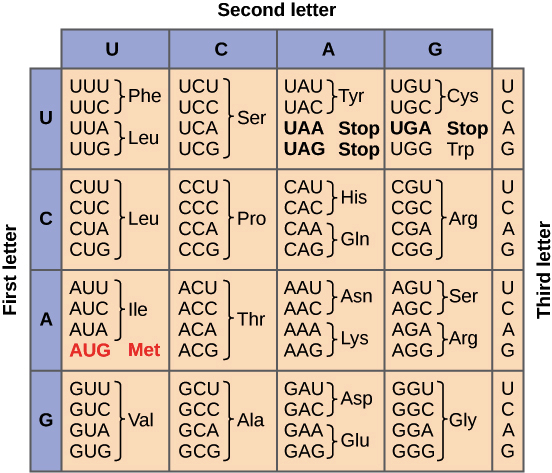
\includegraphics[keepaspectratio]{images/slide-21-image-1.png}}

\end{tcolorbox}

\begin{tcolorbox}[enhanced jigsaw, arc=.35mm, bottomrule=.15mm, bottomtitle=1mm, breakable, colback=white, colbacktitle=quarto-callout-tip-color!10!white, colframe=quarto-callout-tip-color-frame, coltitle=black, left=2mm, leftrule=.75mm, opacityback=0, opacitybacktitle=0.6, rightrule=.15mm, title=\textcolor{quarto-callout-tip-color}{\faLightbulb}\hspace{0.5em}{Answer}, titlerule=0mm, toprule=.15mm, toptitle=1mm]

\begin{itemize}
\tightlist
\item
  The codon so far contains \textbf{G--} and was split by the intron. To
  make it a complete triplet, the rest of the codon must be the
  \emph{-AT} from exon 2.
\item
  GAT.
\item
  Aspartic Acid (D)
\item
  The last two bases are AG
\item
  This is the consensus splice acceptor site.
\end{itemize}

\end{tcolorbox}

Scroll through the gene and note how the intronic sequences are
comprised largely of dispersed repeat sequences.

\pandocbounded{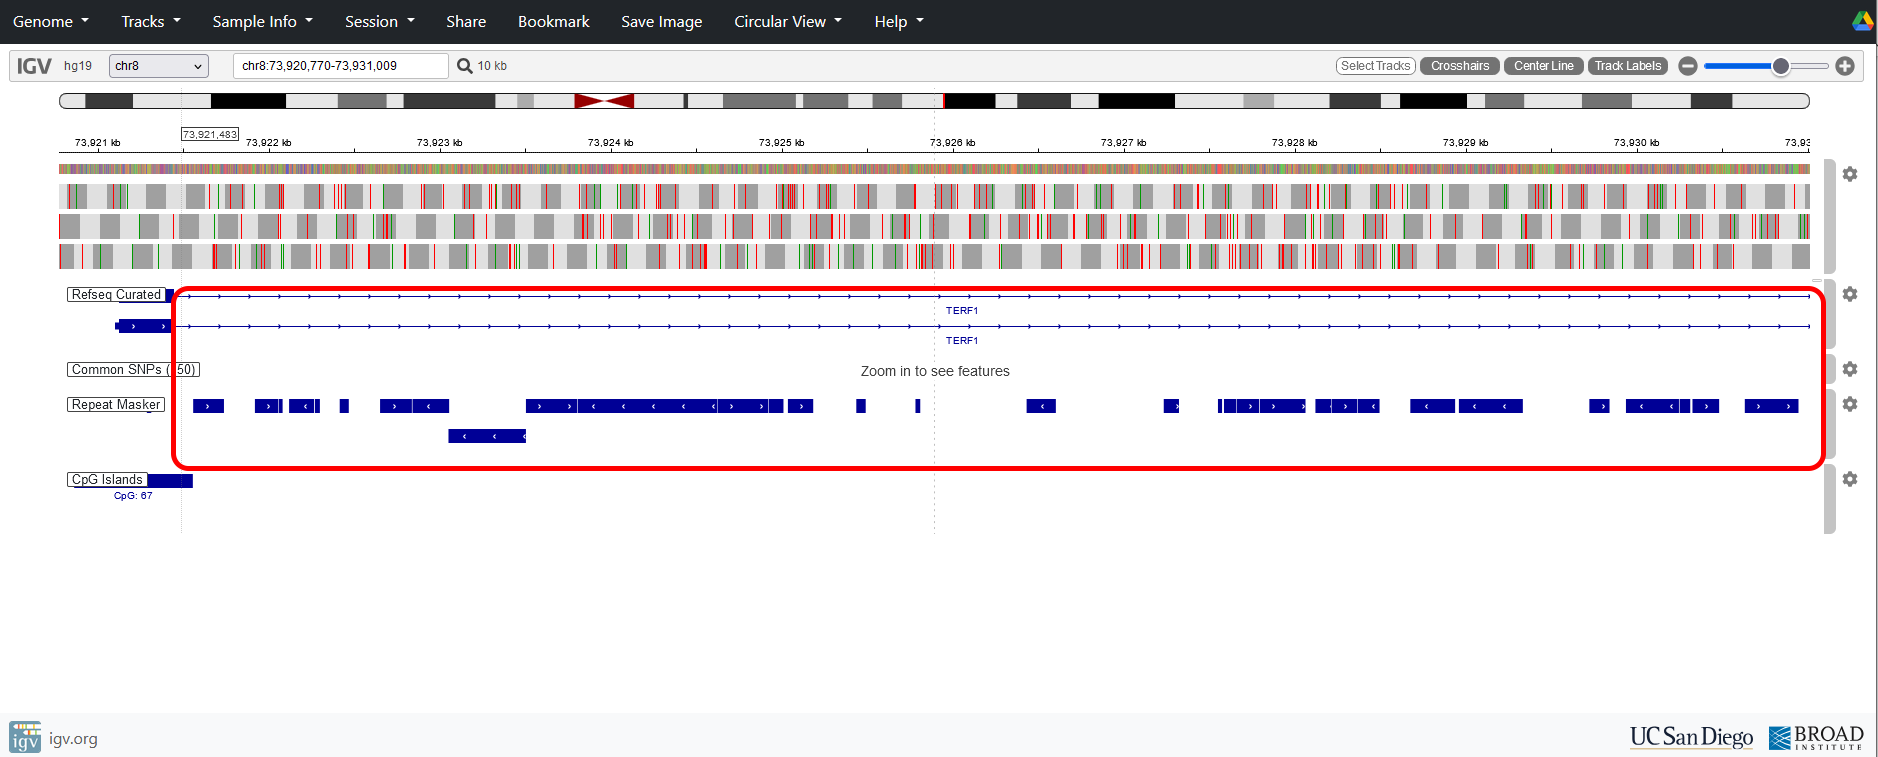
\includegraphics[keepaspectratio]{images/slide-22-image-1.png}}

\section{Examine the terminal exon and 3'
UTR}\label{examine-the-terminal-exon-and-3-utr}

Navigate to the terminal \emph{TERF1} exon and zoom in:

\pandocbounded{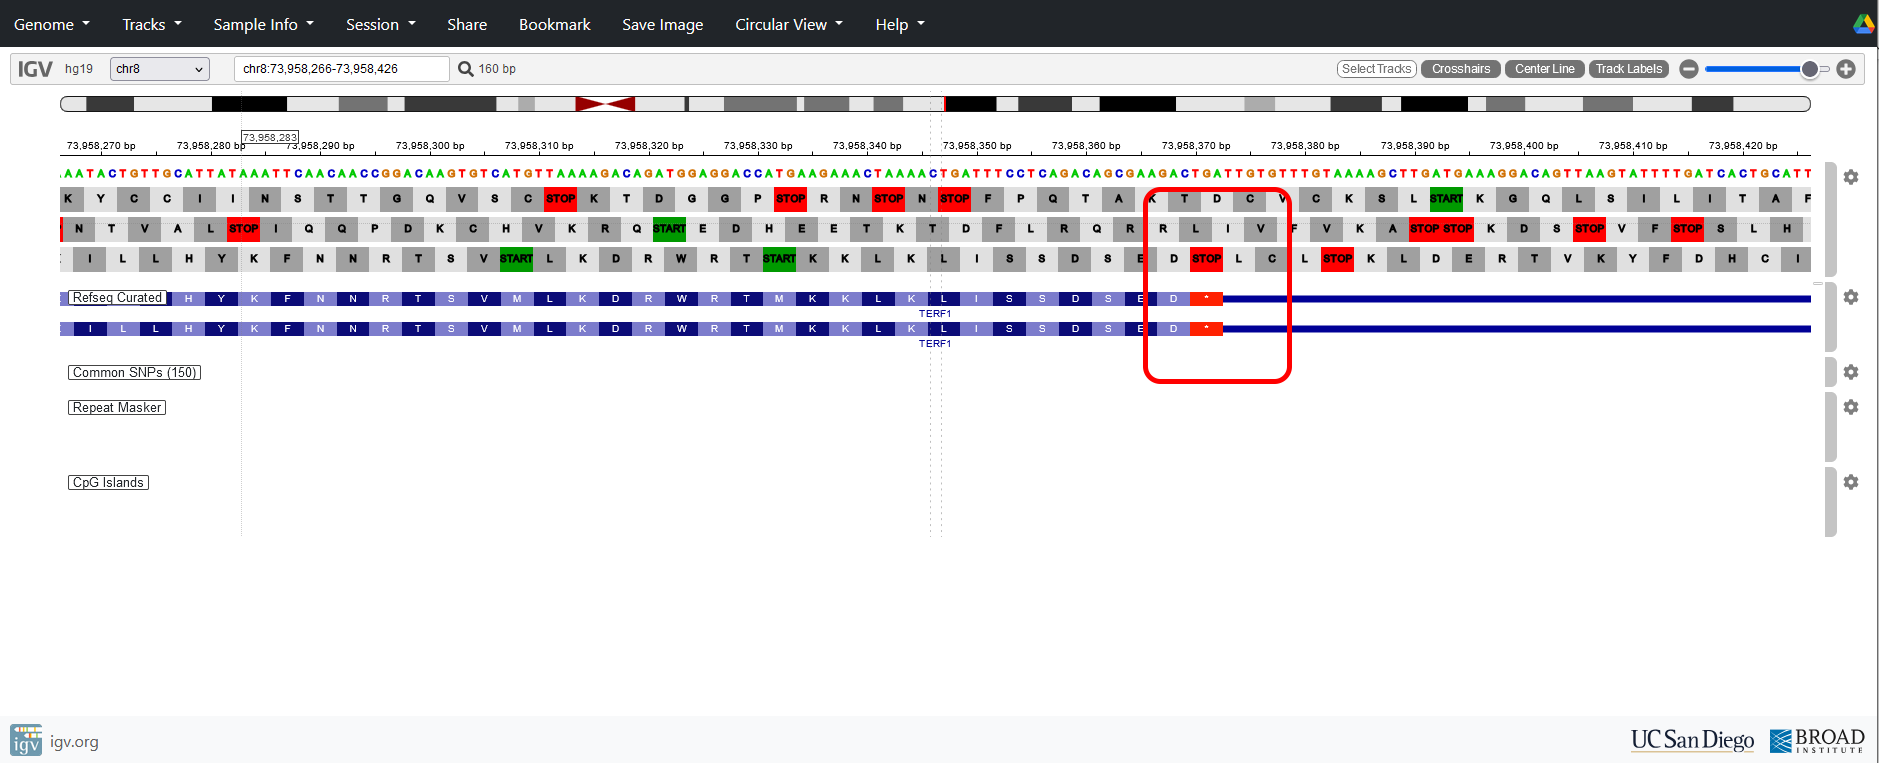
\includegraphics[keepaspectratio]{images/slide-23-image-1.png}}

\begin{tcolorbox}[enhanced jigsaw, arc=.35mm, bottomrule=.15mm, bottomtitle=1mm, breakable, colback=white, colbacktitle=quarto-callout-tip-color!10!white, colframe=quarto-callout-tip-color-frame, coltitle=black, left=2mm, leftrule=.75mm, opacityback=0, opacitybacktitle=0.6, rightrule=.15mm, title=\textcolor{quarto-callout-tip-color}{\faLightbulb}\hspace{0.5em}{Test your understanding}, titlerule=0mm, toprule=.15mm, toptitle=1mm]

\begin{itemize}
\tightlist
\item
  Which is the correct reading frame for this exon in your view?
\item
  What is the sequence of the stop codon?
\end{itemize}

\end{tcolorbox}

\begin{tcolorbox}[enhanced jigsaw, arc=.35mm, bottomrule=.15mm, bottomtitle=1mm, breakable, colback=white, colbacktitle=quarto-callout-tip-color!10!white, colframe=quarto-callout-tip-color-frame, coltitle=black, left=2mm, leftrule=.75mm, opacityback=0, opacitybacktitle=0.6, rightrule=.15mm, title=\textcolor{quarto-callout-tip-color}{\faLightbulb}\hspace{0.5em}{Answer}, titlerule=0mm, toprule=.15mm, toptitle=1mm]

\begin{itemize}
\tightlist
\item
  It will depend on your IGV instance but in this image it is the bottom
  frame as the stop codon coincides with the end of the terminal exon.
\item
  TGA
\end{itemize}

\end{tcolorbox}

Zoom out to see the whole of the final exon.

\pandocbounded{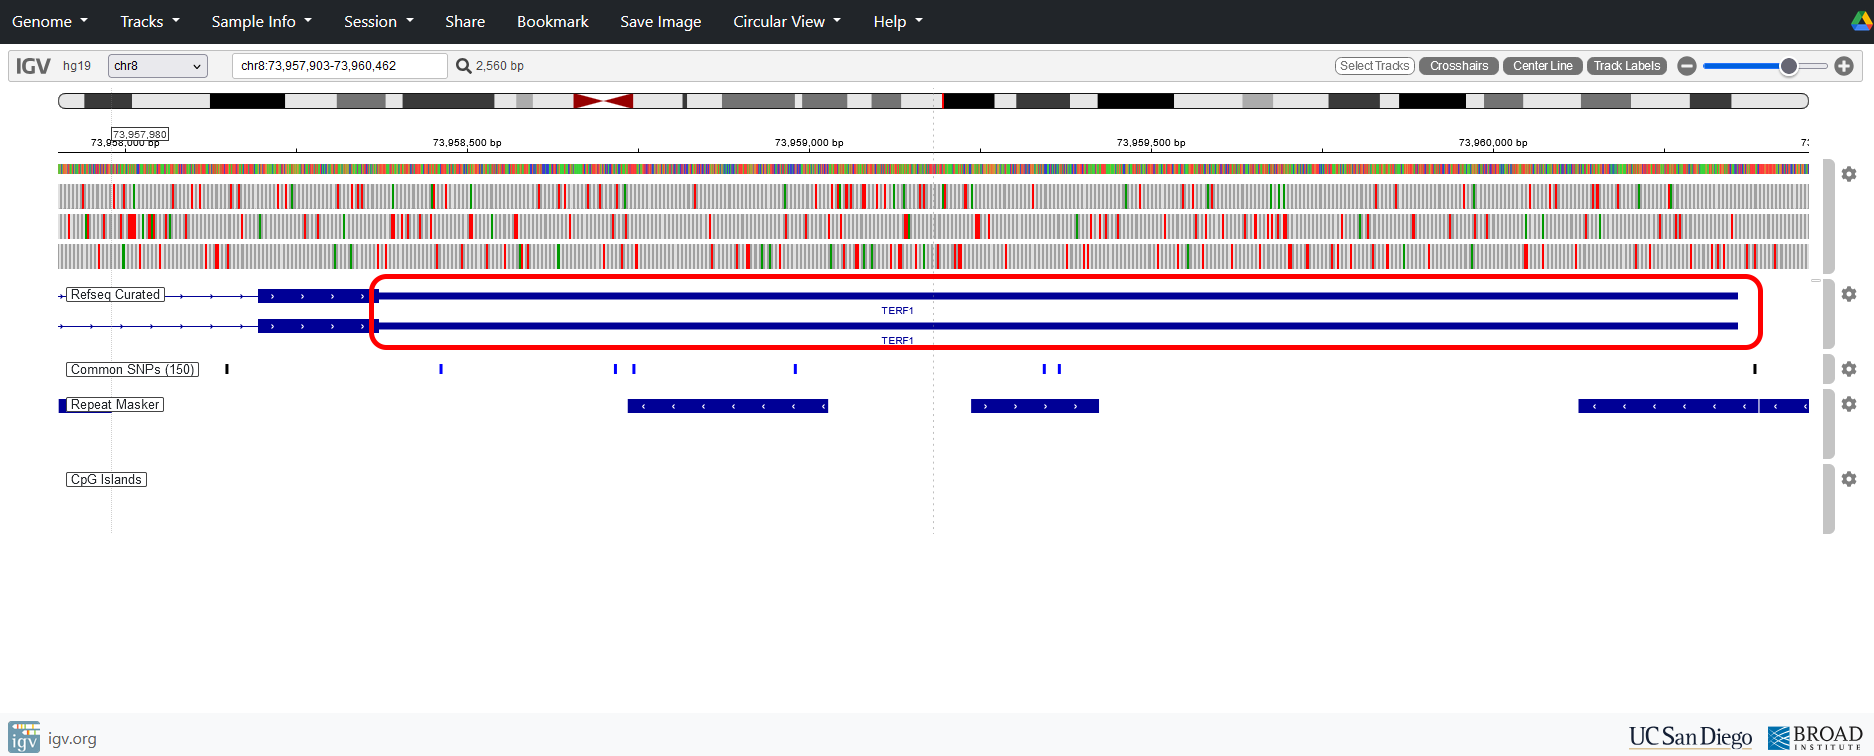
\includegraphics[keepaspectratio]{images/slide-24-image-1.png}}

\begin{tcolorbox}[enhanced jigsaw, arc=.35mm, bottomrule=.15mm, bottomtitle=1mm, breakable, colback=white, colbacktitle=quarto-callout-tip-color!10!white, colframe=quarto-callout-tip-color-frame, coltitle=black, left=2mm, leftrule=.75mm, opacityback=0, opacitybacktitle=0.6, rightrule=.15mm, title=\textcolor{quarto-callout-tip-color}{\faLightbulb}\hspace{0.5em}{Test your understanding}, titlerule=0mm, toprule=.15mm, toptitle=1mm]

\begin{itemize}
\tightlist
\item
  What is the approximate length of the 3' UTR for \emph{TERF1}?
\end{itemize}

\end{tcolorbox}

\begin{tcolorbox}[enhanced jigsaw, arc=.35mm, bottomrule=.15mm, bottomtitle=1mm, breakable, colback=white, colbacktitle=quarto-callout-tip-color!10!white, colframe=quarto-callout-tip-color-frame, coltitle=black, left=2mm, leftrule=.75mm, opacityback=0, opacitybacktitle=0.6, rightrule=.15mm, title=\textcolor{quarto-callout-tip-color}{\faLightbulb}\hspace{0.5em}{Answer}, titlerule=0mm, toprule=.15mm, toptitle=1mm]

The UTR spans 73,960,358 to 73,958,372 so is 1,986 bases (approx. 2,000
bp)

\end{tcolorbox}

\bookmarksetup{startatroot}

\chapter{\texorpdfstring{Genes on the reverse strand:
\emph{DMPK}}{Genes on the reverse strand: DMPK}}\label{genes-on-the-reverse-strand-dmpk}

Let's look at the \emph{DMPK} gene. This gene is different from
\emph{TERF1} as it is transcribed from the bottom strand relative to the
chromosomal reference (the top strand). Exon 1 is on the right, and the
terminal exon on the left. You can quickly navigate to \emph{DMPK} (or
any gene) by typing its name into the search bar.

\pandocbounded{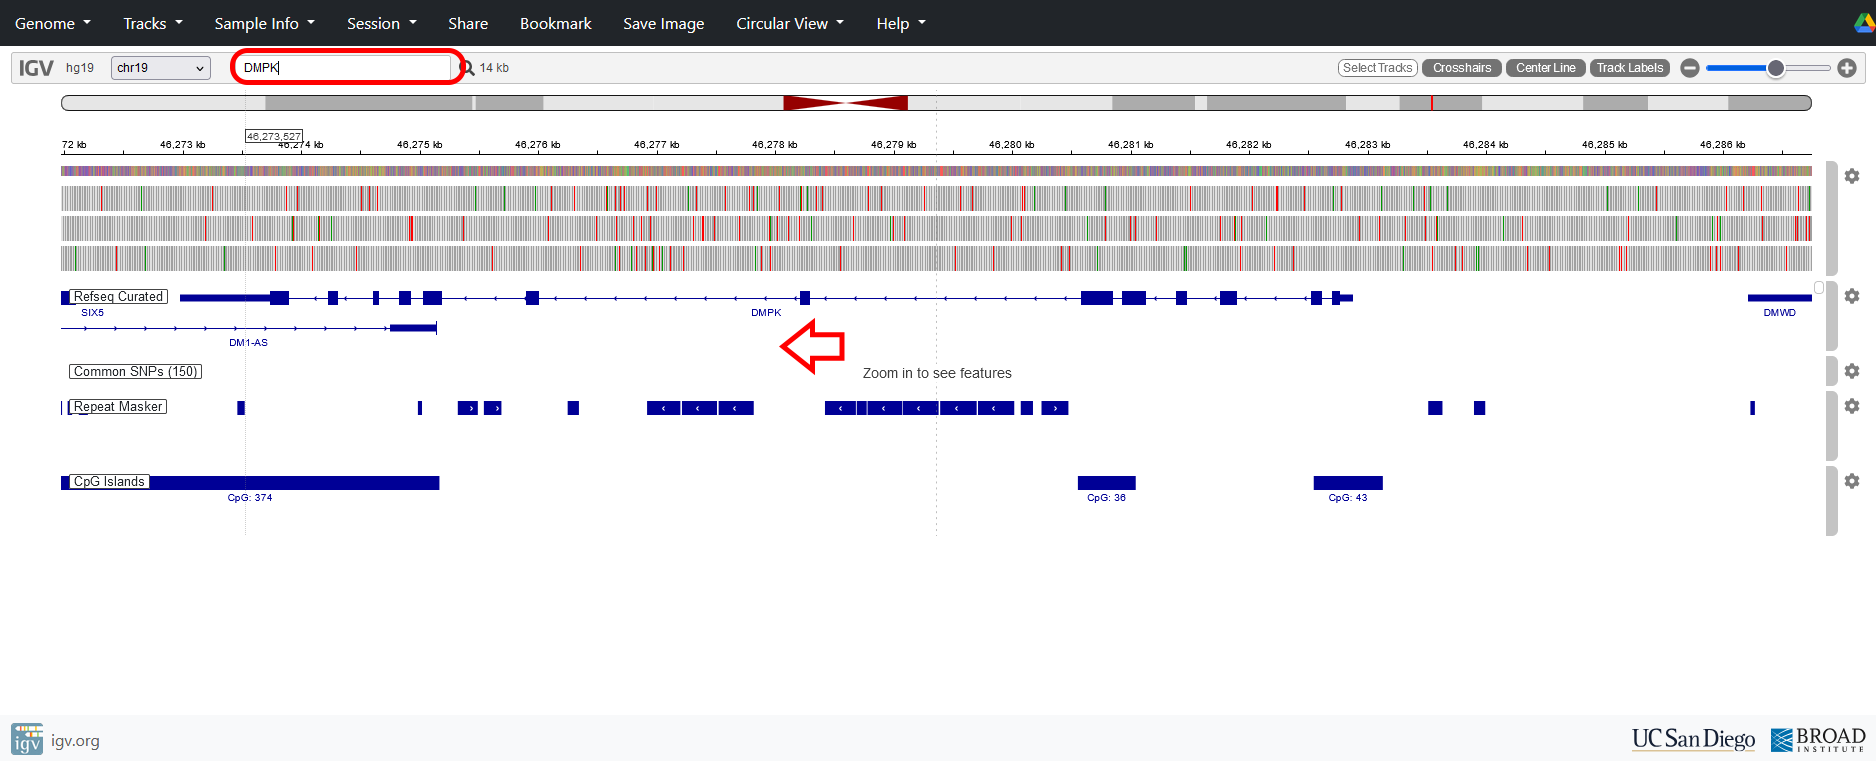
\includegraphics[keepaspectratio]{images/slide-25-image-1.png}}

Zoom in on one of the DMPK coding exons. To see the correct amino acid
sequence for this gene, we will have to set the `reverse' option so that
IGV translates from the bottom strand. Remember that it will still be
running right to left.

\begin{tcolorbox}[enhanced jigsaw, arc=.35mm, bottomrule=.15mm, bottomtitle=1mm, breakable, colback=white, colbacktitle=quarto-callout-warning-color!10!white, colframe=quarto-callout-warning-color-frame, coltitle=black, left=2mm, leftrule=.75mm, opacityback=0, opacitybacktitle=0.6, rightrule=.15mm, title=\textcolor{quarto-callout-warning-color}{\faExclamationTriangle}\hspace{0.5em}{Warning}, titlerule=0mm, toprule=.15mm, toptitle=1mm]

Don't forget to turn this option off again if you look at a gene or
variants on the reference (top) strand.

\end{tcolorbox}

\pandocbounded{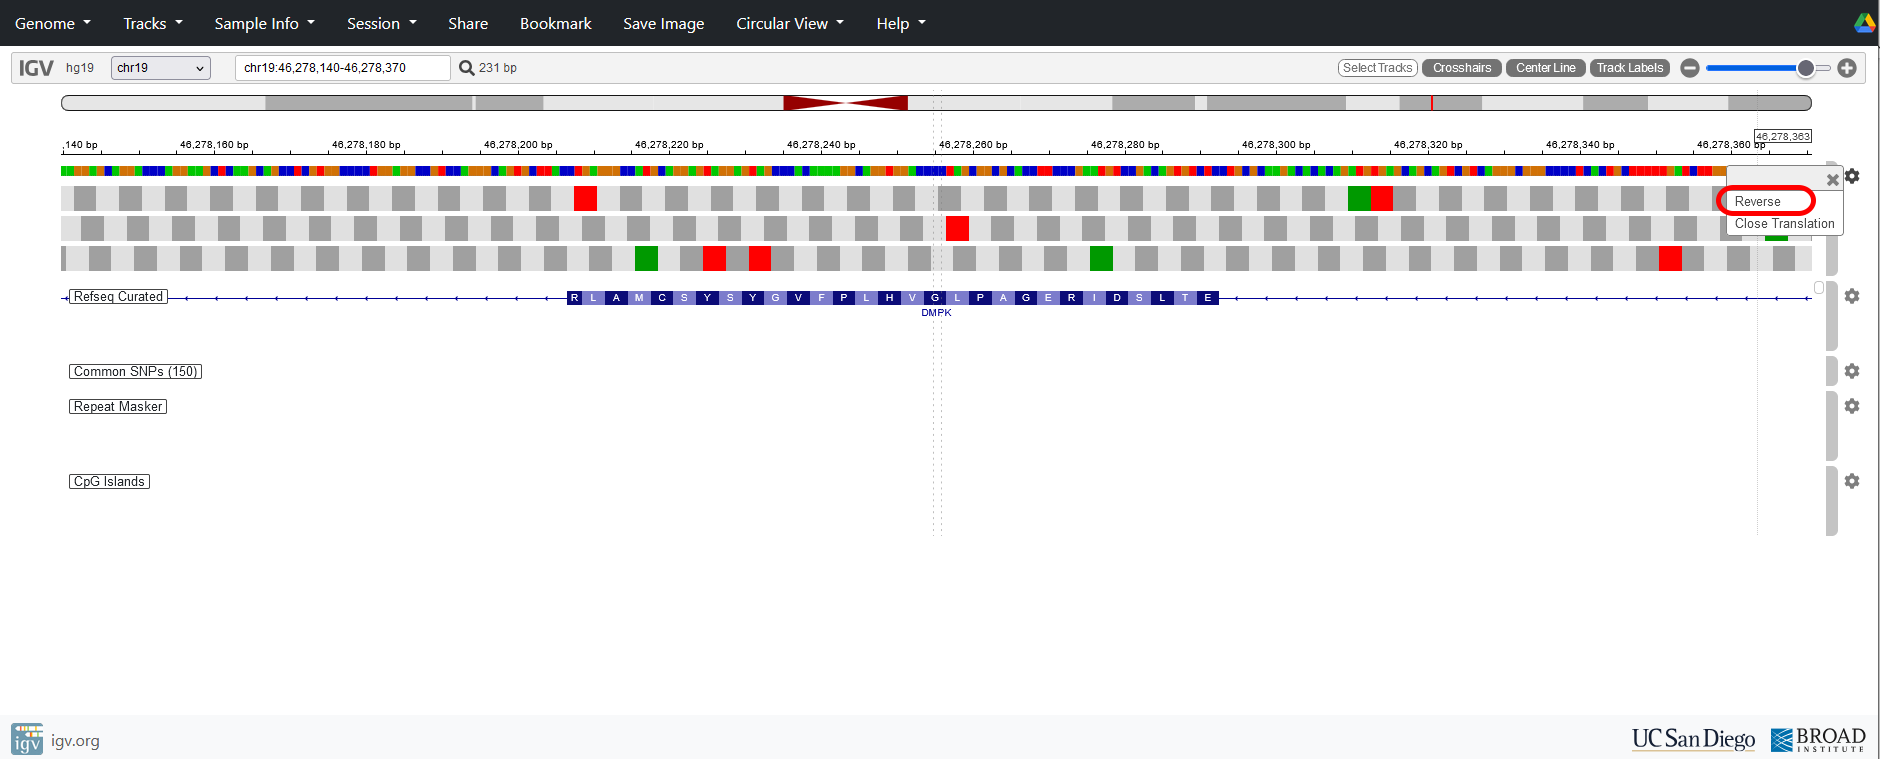
\includegraphics[keepaspectratio]{images/slide-26-image-1.png}}

Zoom out a bit more to get an overview of the other genes in the
vicinity of \emph{DMPK}. Some genes are in the same orientation as DMPK
and transcribed from the bottom strand (e.g.~\emph{SIX5}, \emph{DMWD},
\emph{RSPH6A}) but others are transcribed from the top strand
(e.g.~\emph{BHMG1}).

You should also see that many genes have a CpG island spanning exon 1.
These regions are often (but not always) associated with the presence of
H3K4me3 in ChIP-seq data, indicating open chromatin.

\pandocbounded{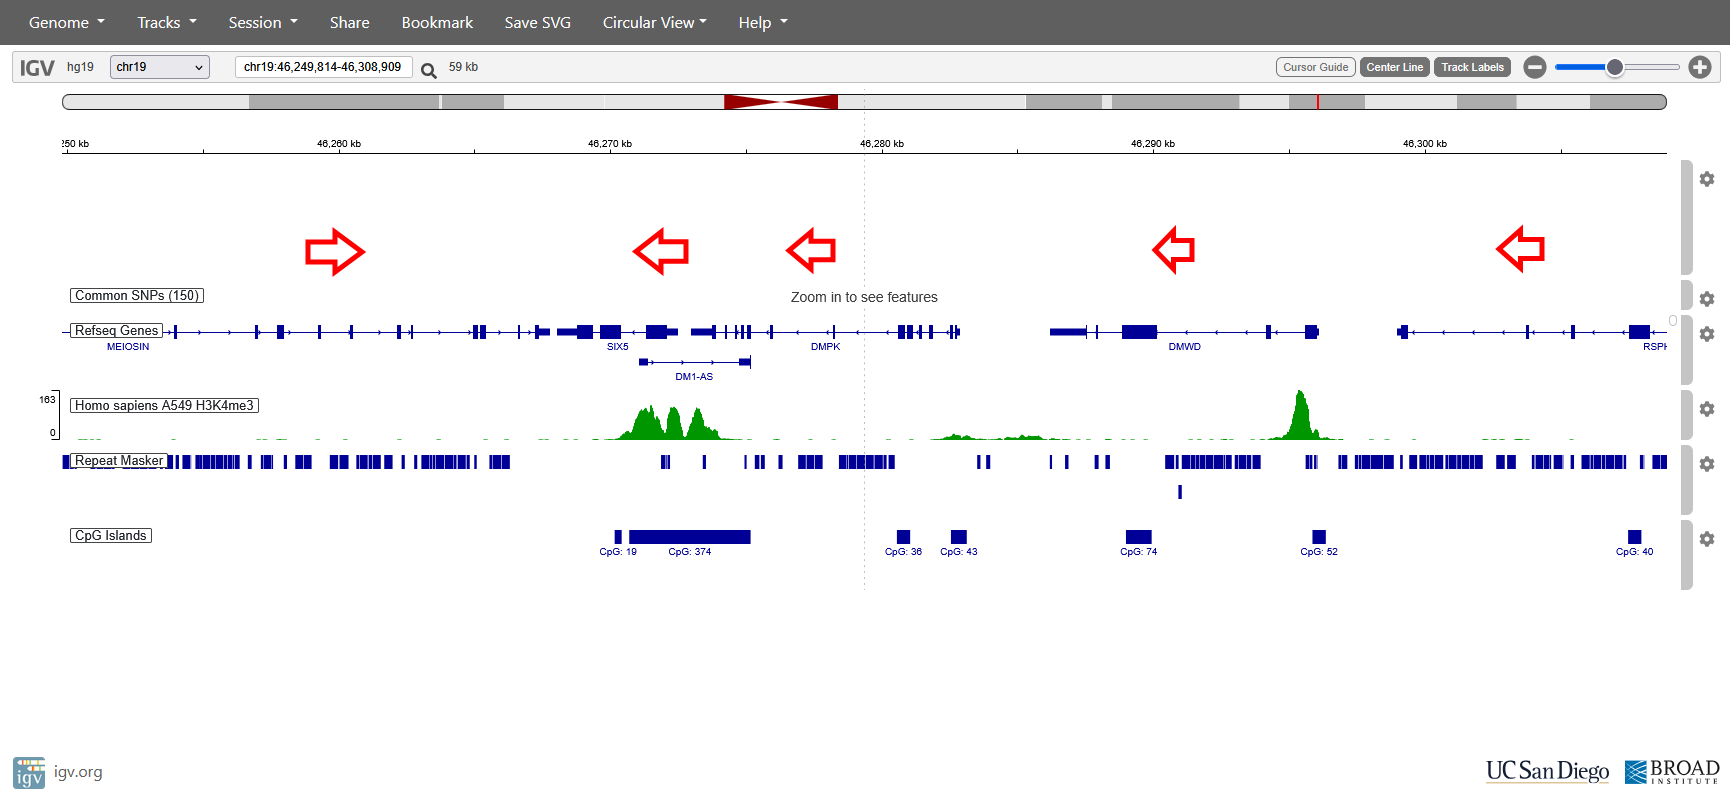
\includegraphics[keepaspectratio]{images/slide-27-image-1.png}}

\bookmarksetup{startatroot}

\chapter{Load Platinum Genomes sequencing
data}\label{load-platinum-genomes-sequencing-data}

Next, we will load some actual sequence data from the platinum genomes
collection of tracks:

\pandocbounded{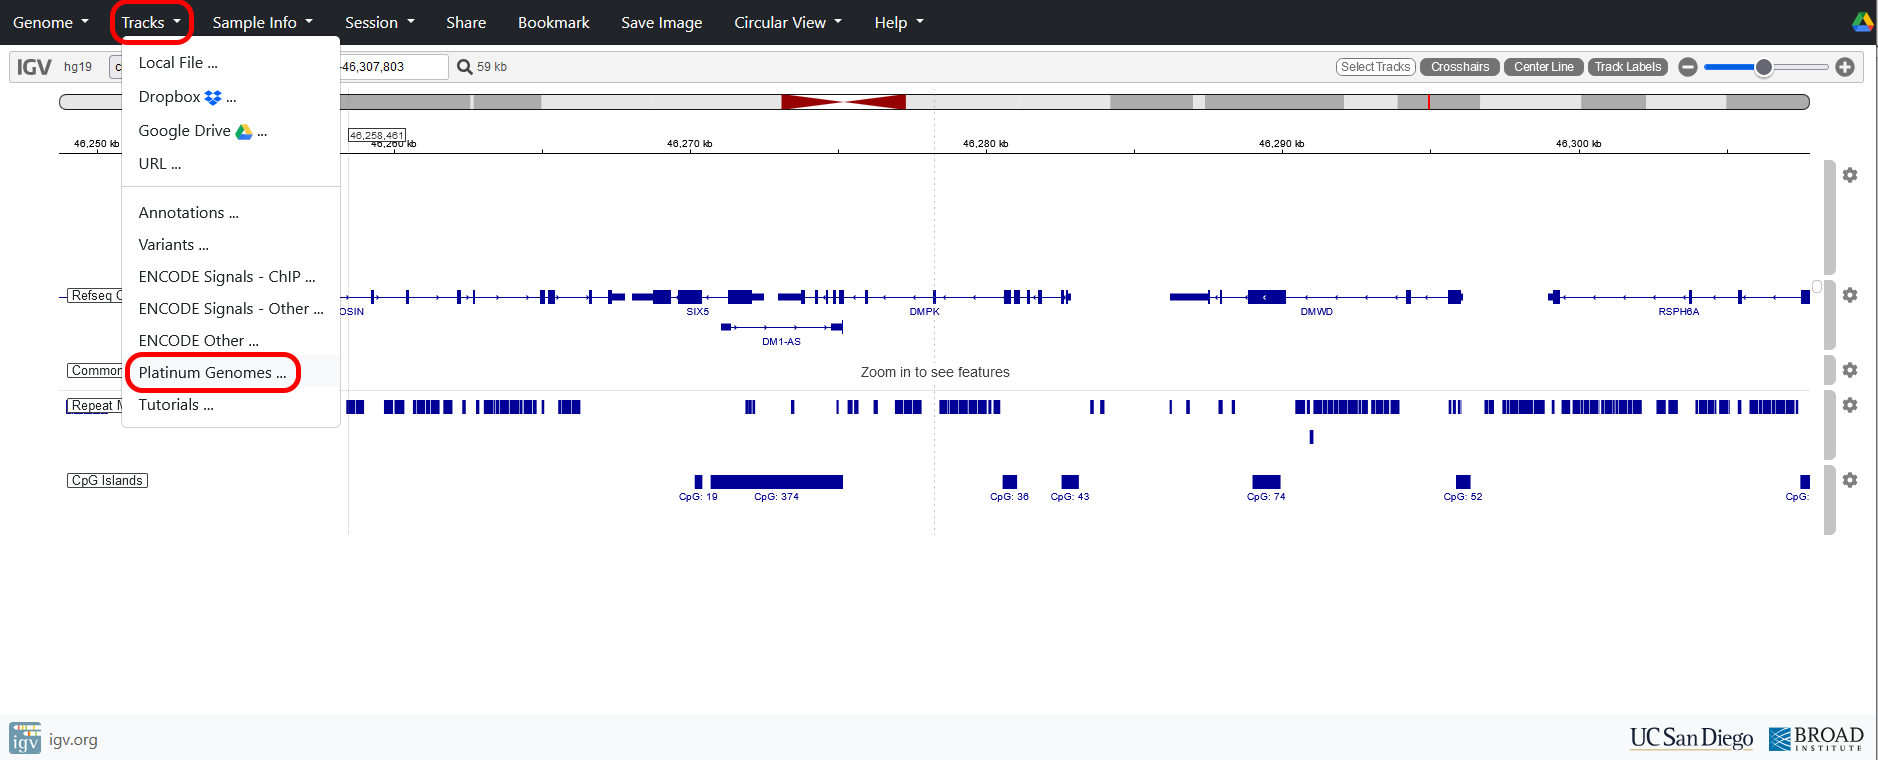
\includegraphics[keepaspectratio]{images/slide-28-image-1.png}}

Shift-click samples \textbf{NA12889}, \textbf{NA12890} and
\textbf{NA12877} and press OK.

\pandocbounded{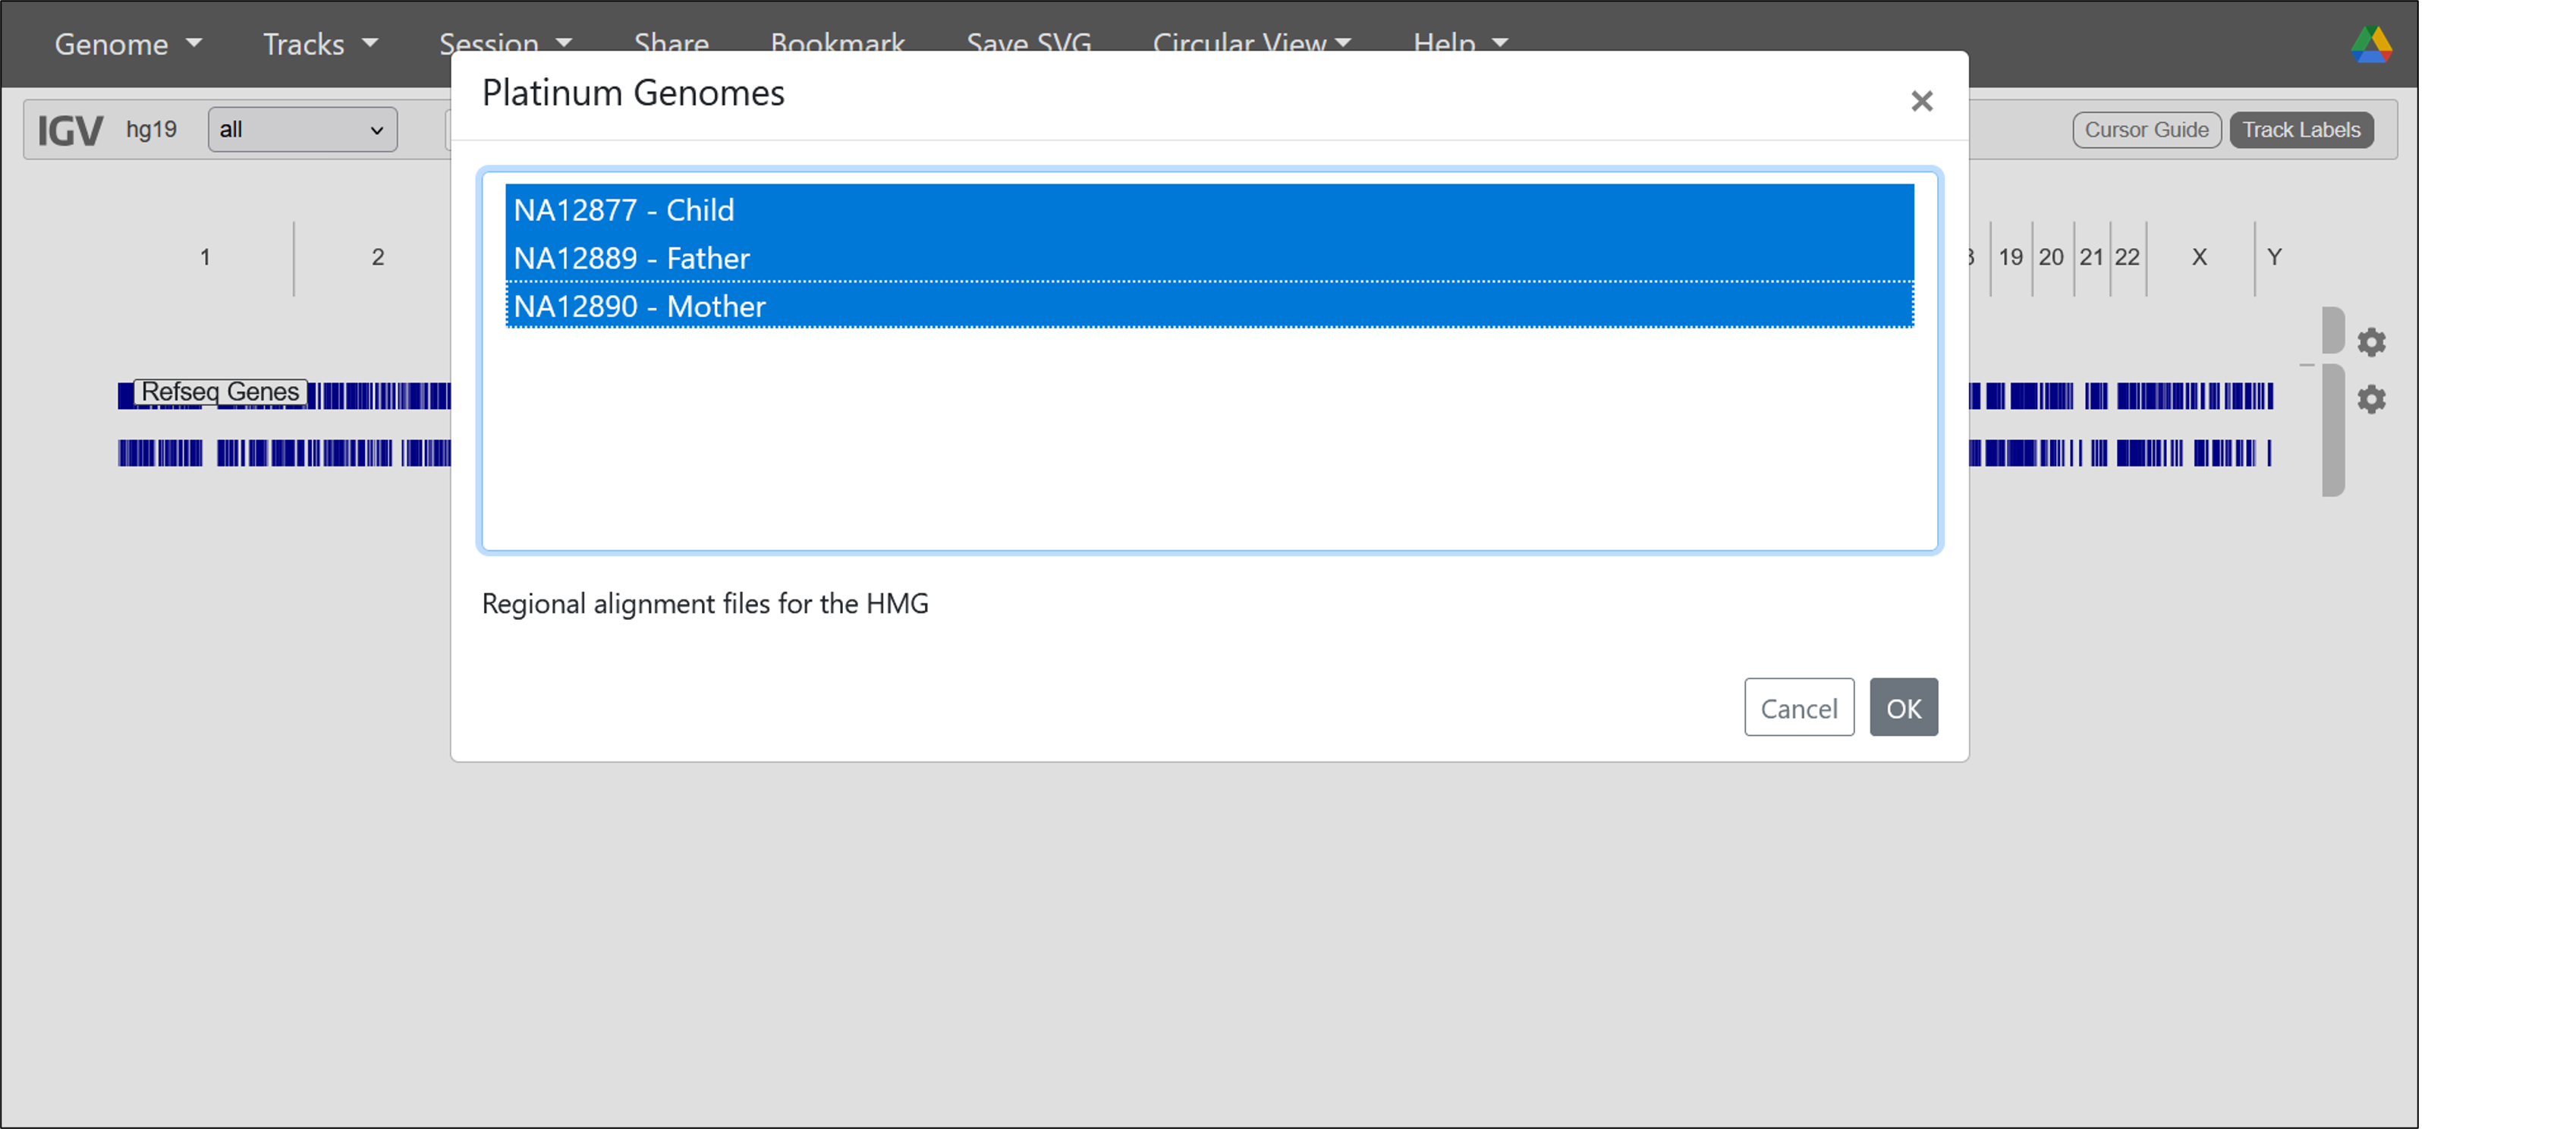
\includegraphics[keepaspectratio]{images/slide-29-image-1.png}}

The platinum genomes are derived from a reference genome dataset
described in \href{https://genome.cshlp.org/content/27/1/157}{Eberle
\emph{et al., 2017}}. In the study, the genomes of four grandparents,
two parents and 11 children were sequenced on an Illumina HiSeq2000 to
an average depth of 50× using 2×100 bp paired-end reads.

The ID of each sample is defined by adding the family identifier prefix
(e.g.~NA128) to each numbered individual (e.g.~77 would be NA12877). For
this session, we will load in a mother-father-child family trio
(individuals 89, 90 and 77) from family NA128.

\pandocbounded{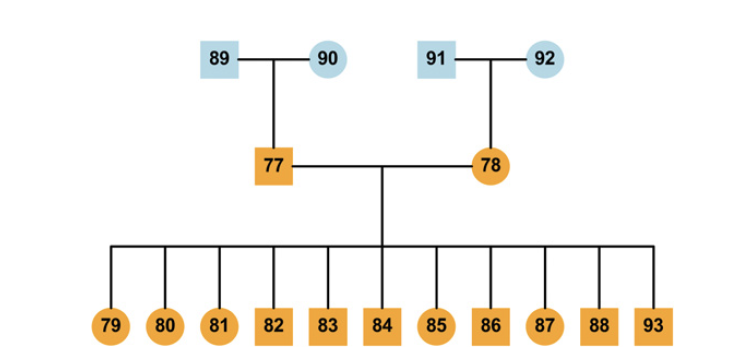
\includegraphics[keepaspectratio]{images/slide-30-image-1.png}}

You may need to use the cog associated with each track to change the
Track Height to get everything visible on your screen. You can also drag
the tracks into an easier order using the handles at the side of each
track.

\pandocbounded{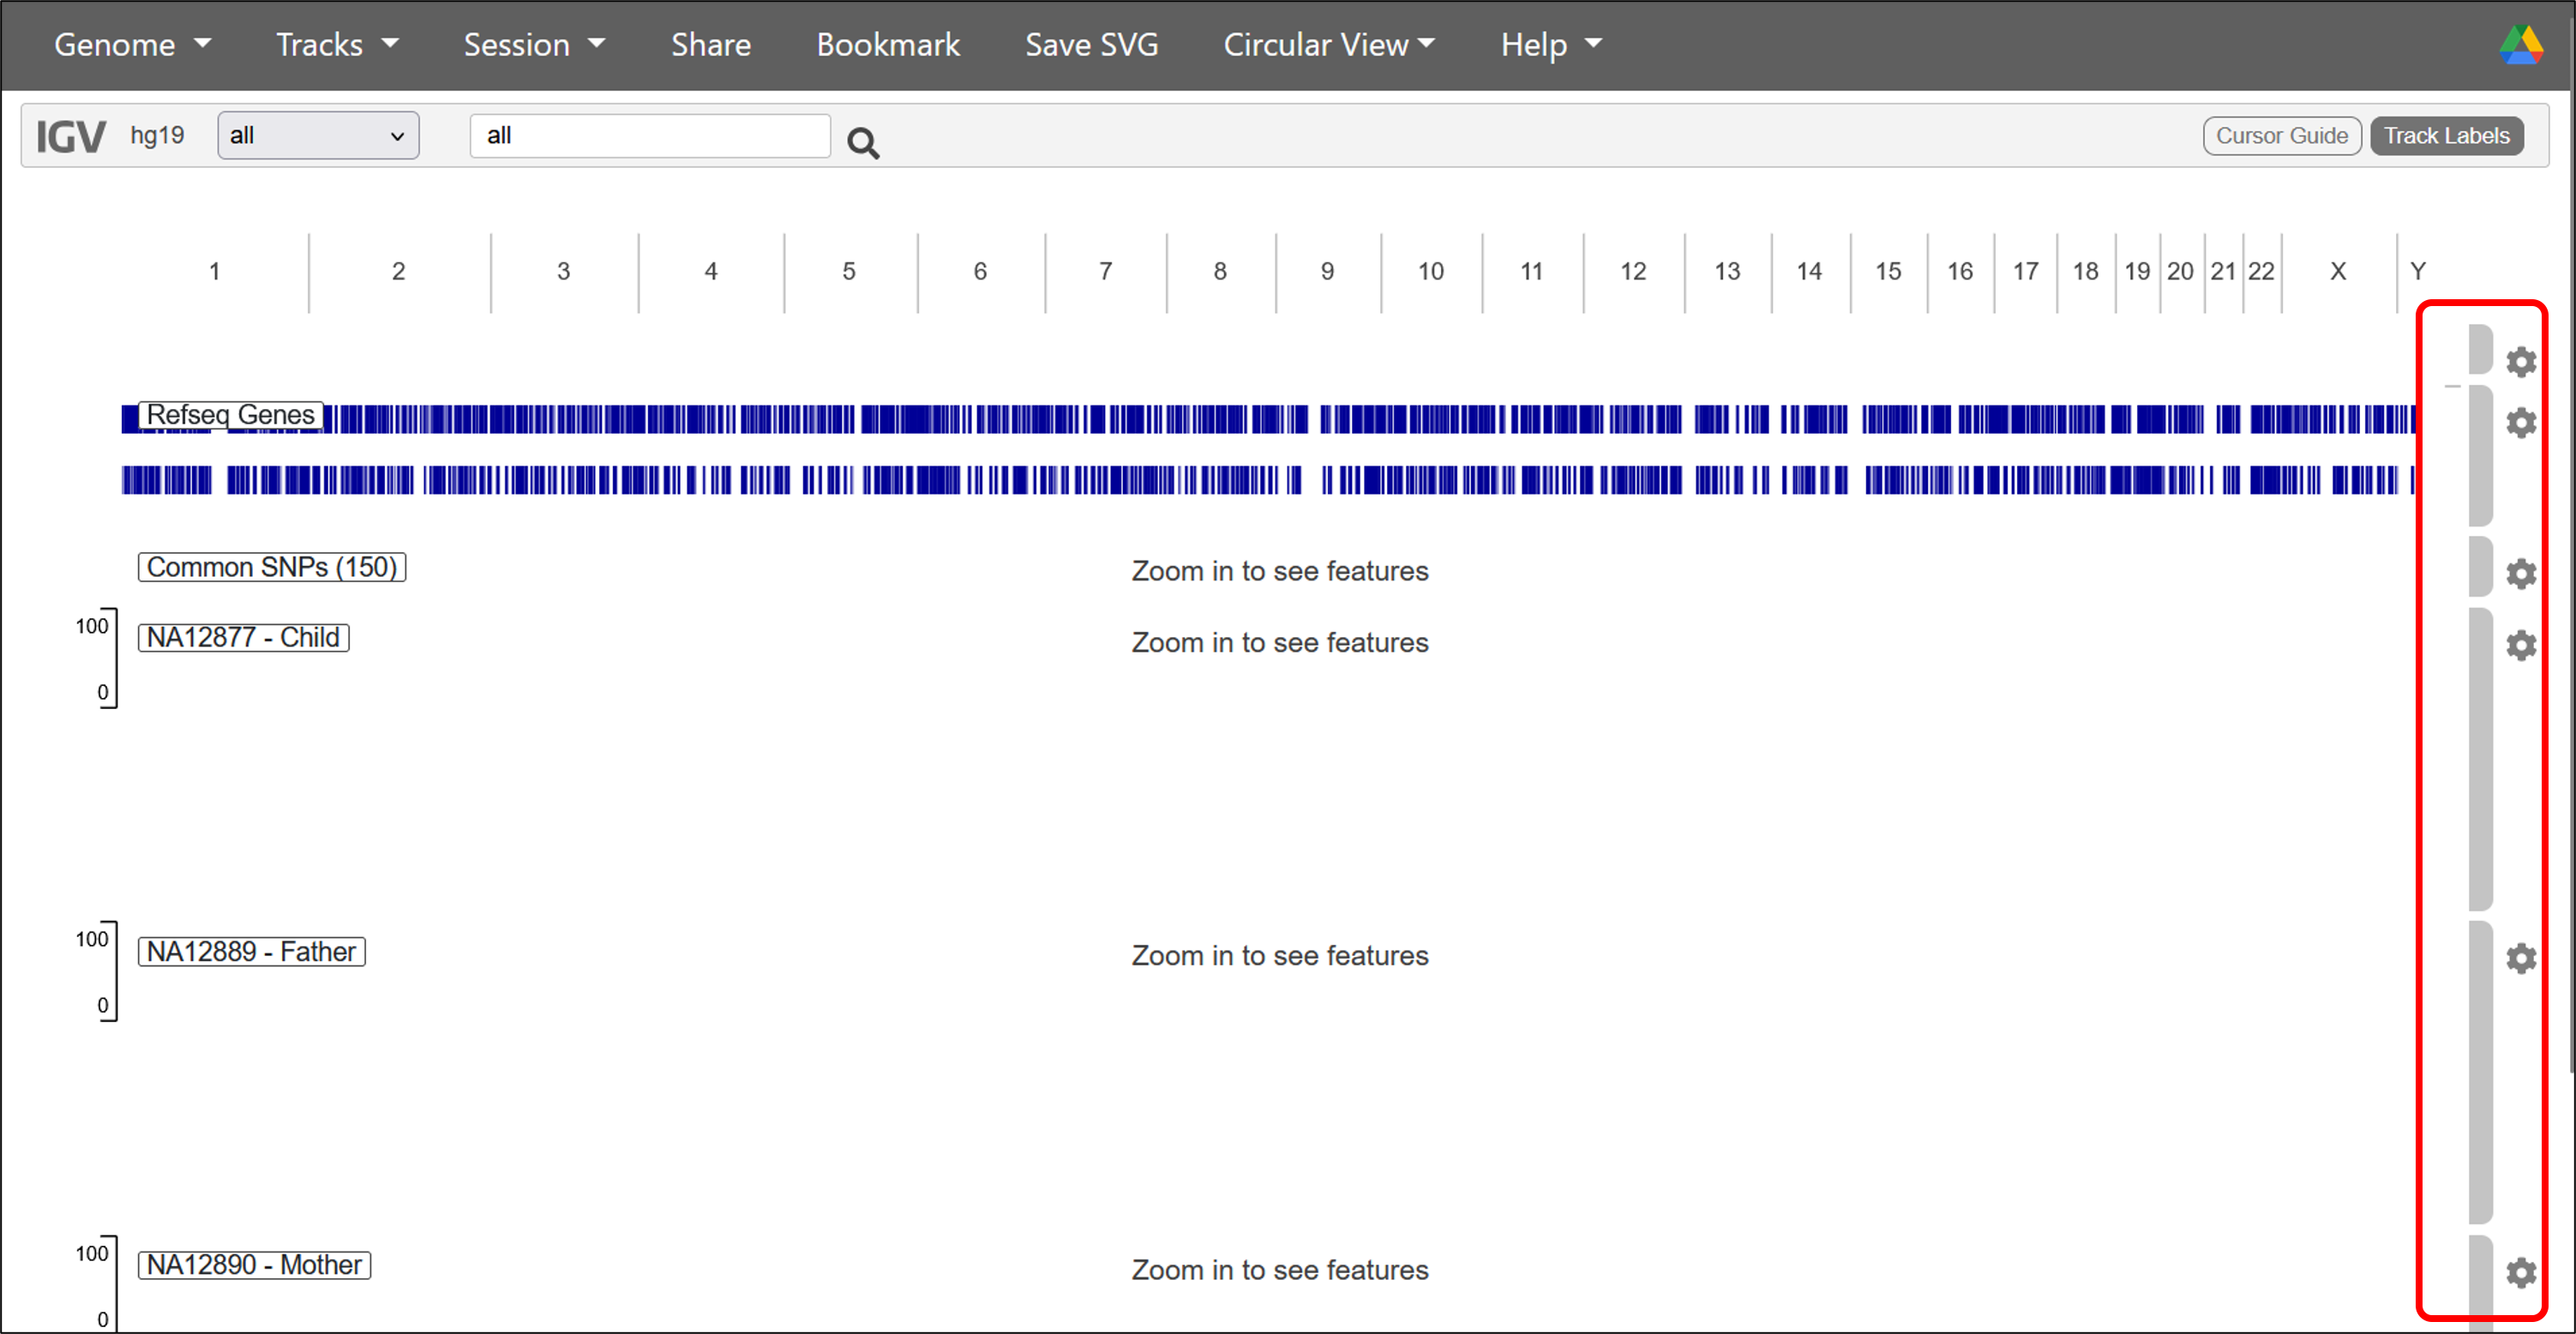
\includegraphics[keepaspectratio]{images/slide-31-image-2.png}}

We can speed up the display by removing tracks we no longer need
(e.g.~CpG, repeats and H3K4me3) by clicking their specific cog on the
track and selecting remove.

\pandocbounded{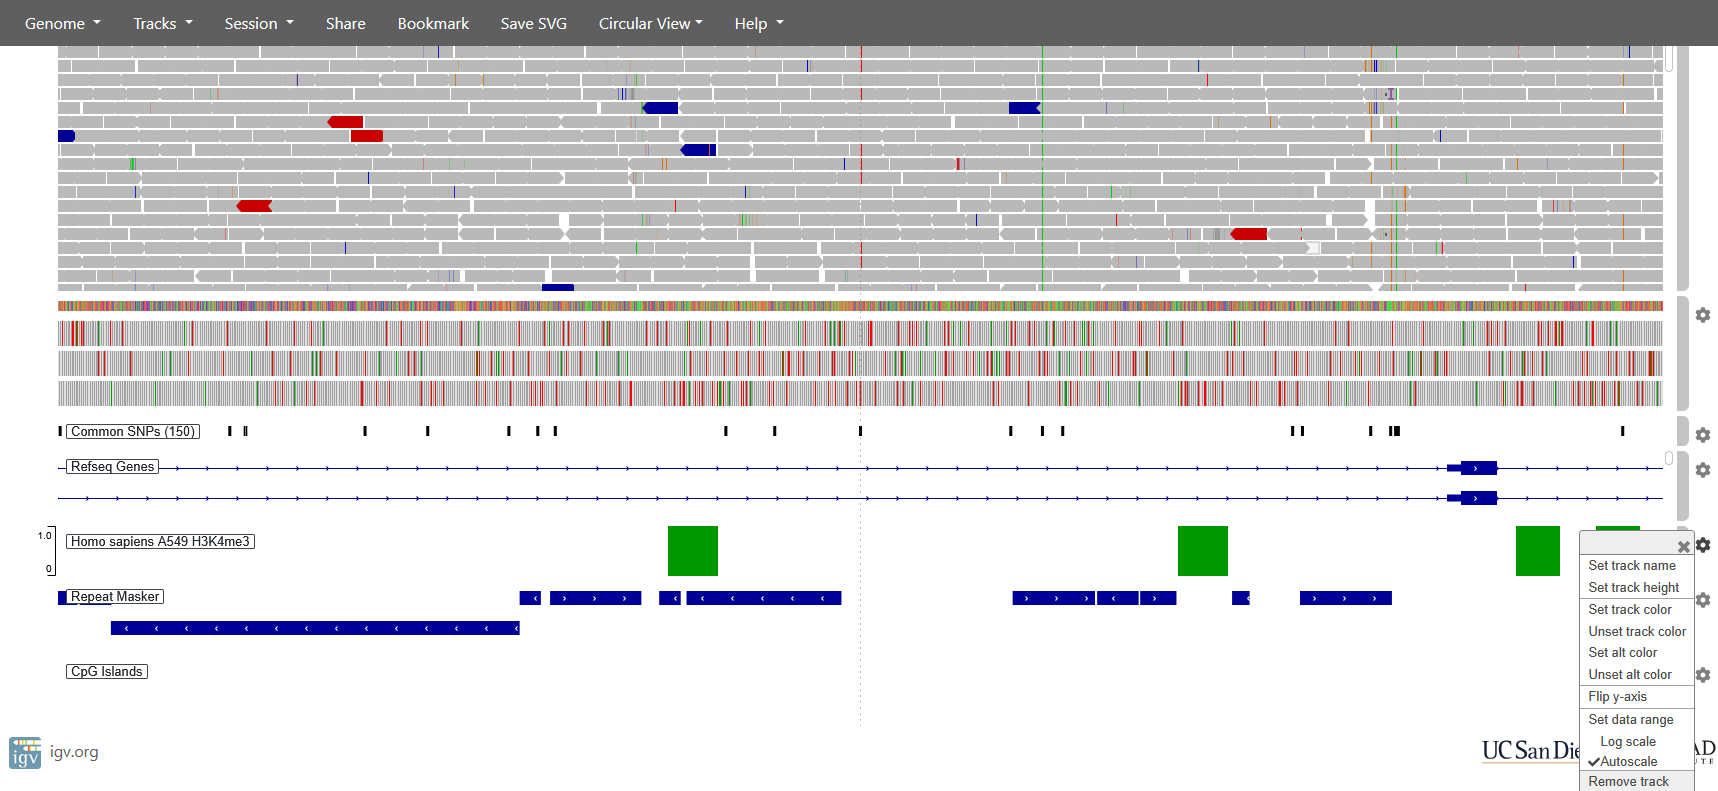
\includegraphics[keepaspectratio]{images/slide-32-image-1.png}}

\begin{tcolorbox}[enhanced jigsaw, arc=.35mm, bottomrule=.15mm, bottomtitle=1mm, breakable, colback=white, colbacktitle=quarto-callout-warning-color!10!white, colframe=quarto-callout-warning-color-frame, coltitle=black, left=2mm, leftrule=.75mm, opacityback=0, opacitybacktitle=0.6, rightrule=.15mm, title=\textcolor{quarto-callout-warning-color}{\faExclamationTriangle}\hspace{0.5em}{Warning}, titlerule=0mm, toprule=.15mm, toptitle=1mm]

Sometimes IGV still slows down when you load the sequence data and you
may need to refresh the page if it gets stuck. Unfortunately, you will
then need to change the genome to hg19 again and reload the relevant
tracks again.

\end{tcolorbox}

\bookmarksetup{startatroot}

\chapter{\texorpdfstring{Inspect reads and identify variants in
\emph{MYO6}}{Inspect reads and identify variants in MYO6}}\label{inspect-reads-and-identify-variants-in-myo6}

Let's zoom in and have a look at a region in the \emph{MYO6} gene of the
trio in detail by typing the chromosome coordinates into the search box:
chr6:76,525,195-76,525,426.

\emph{MYO6} mutations are linked to autosomal dominant and autosomal
recessive inherited hearing loss.

\begin{tcolorbox}[enhanced jigsaw, arc=.35mm, bottomrule=.15mm, bottomtitle=1mm, breakable, colback=white, colbacktitle=quarto-callout-warning-color!10!white, colframe=quarto-callout-warning-color-frame, coltitle=black, left=2mm, leftrule=.75mm, opacityback=0, opacitybacktitle=0.6, rightrule=.15mm, title=\textcolor{quarto-callout-warning-color}{\faExclamationTriangle}\hspace{0.5em}{Warning}, titlerule=0mm, toprule=.15mm, toptitle=1mm]

We will be examining variants in the top reference strand, so it is best
to turn off the `reverse' option for this region unless looking at
whether a variant is synonymous

\end{tcolorbox}

\pandocbounded{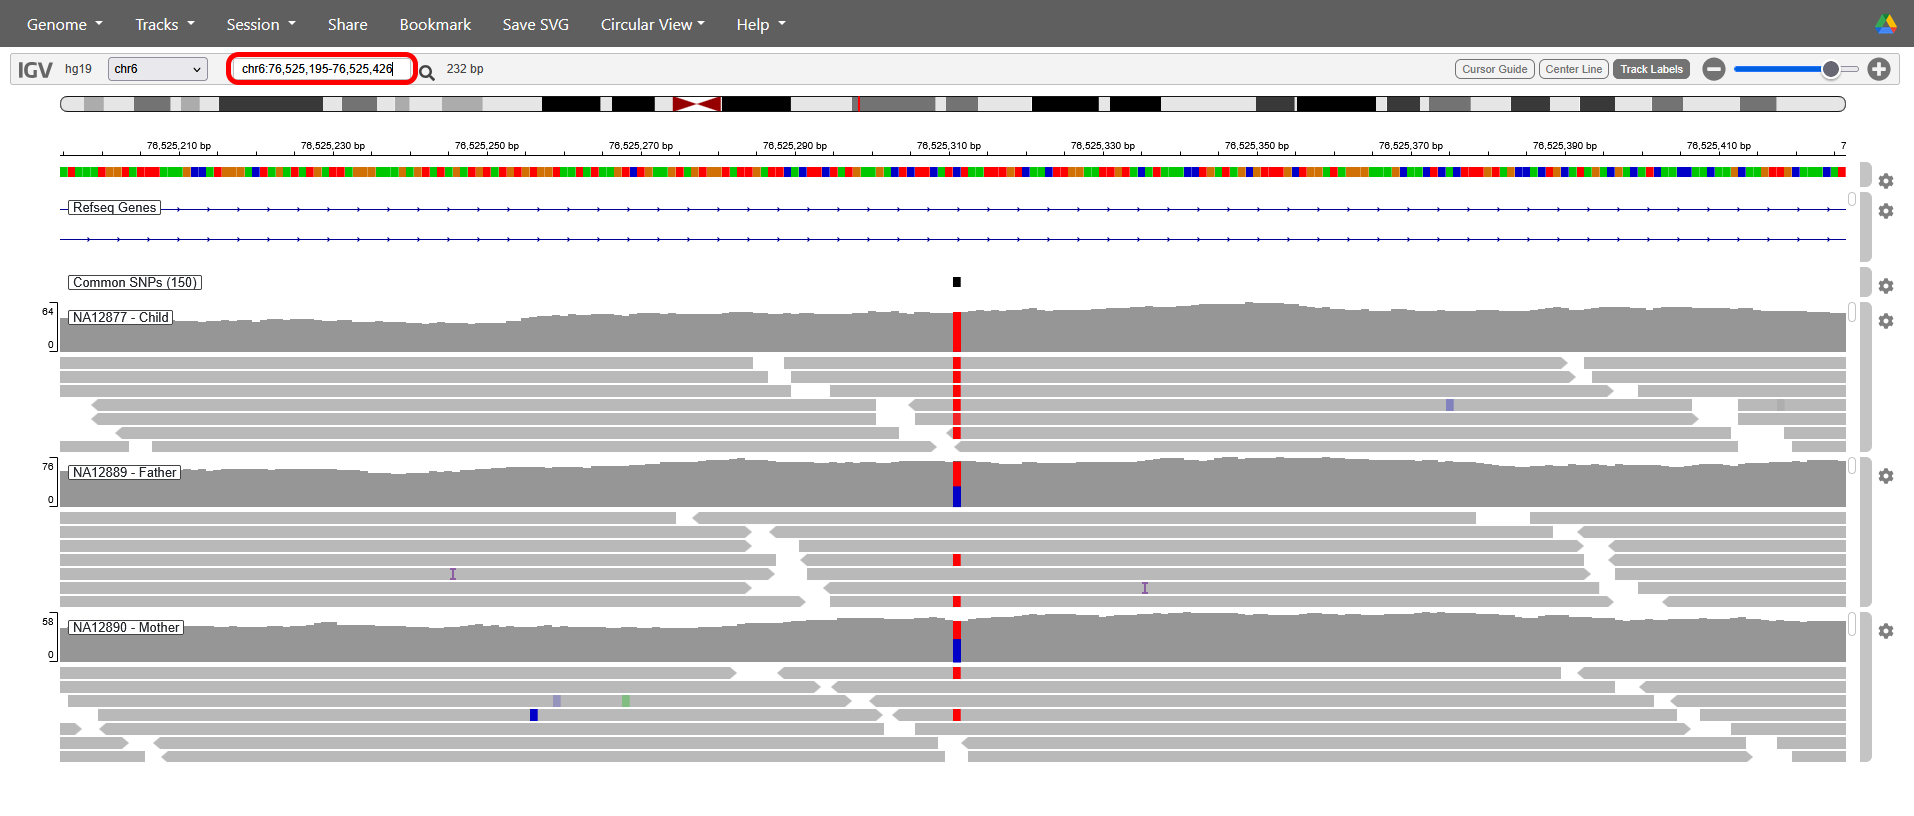
\includegraphics[keepaspectratio]{images/slide-33-image-1.png}}

The mountain plot at the top of the display shows the read depth across
the region (the scale here goes from 0 to 52x). Individual 100 bp reads
are shown as grey rectangles - the arrow on the end indicating the
direction of the read (you can use the scroll bar here to see more of
the reads).

\begin{itemize}
\tightlist
\item
  Where a base in a read is the same as the reference, it is coloured
  grey
\item
  Where a base in a read is different to the reference, it is coloured
  by base.
\end{itemize}

\pandocbounded{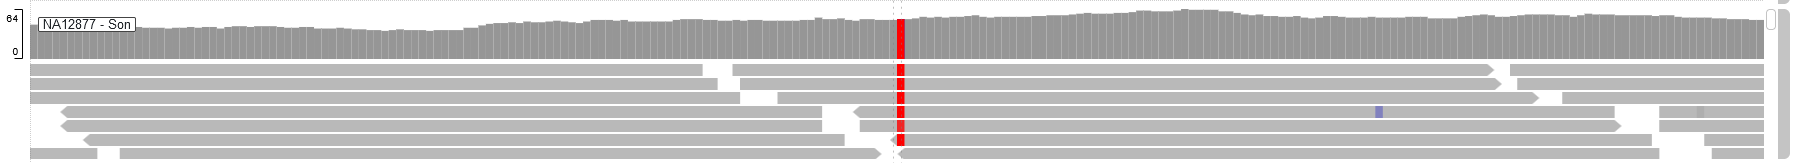
\includegraphics[keepaspectratio]{images/slide-34-image-2.png}}

Zooming in even closer we can see the actual sequences and identify any
differences between the reads and the reference.

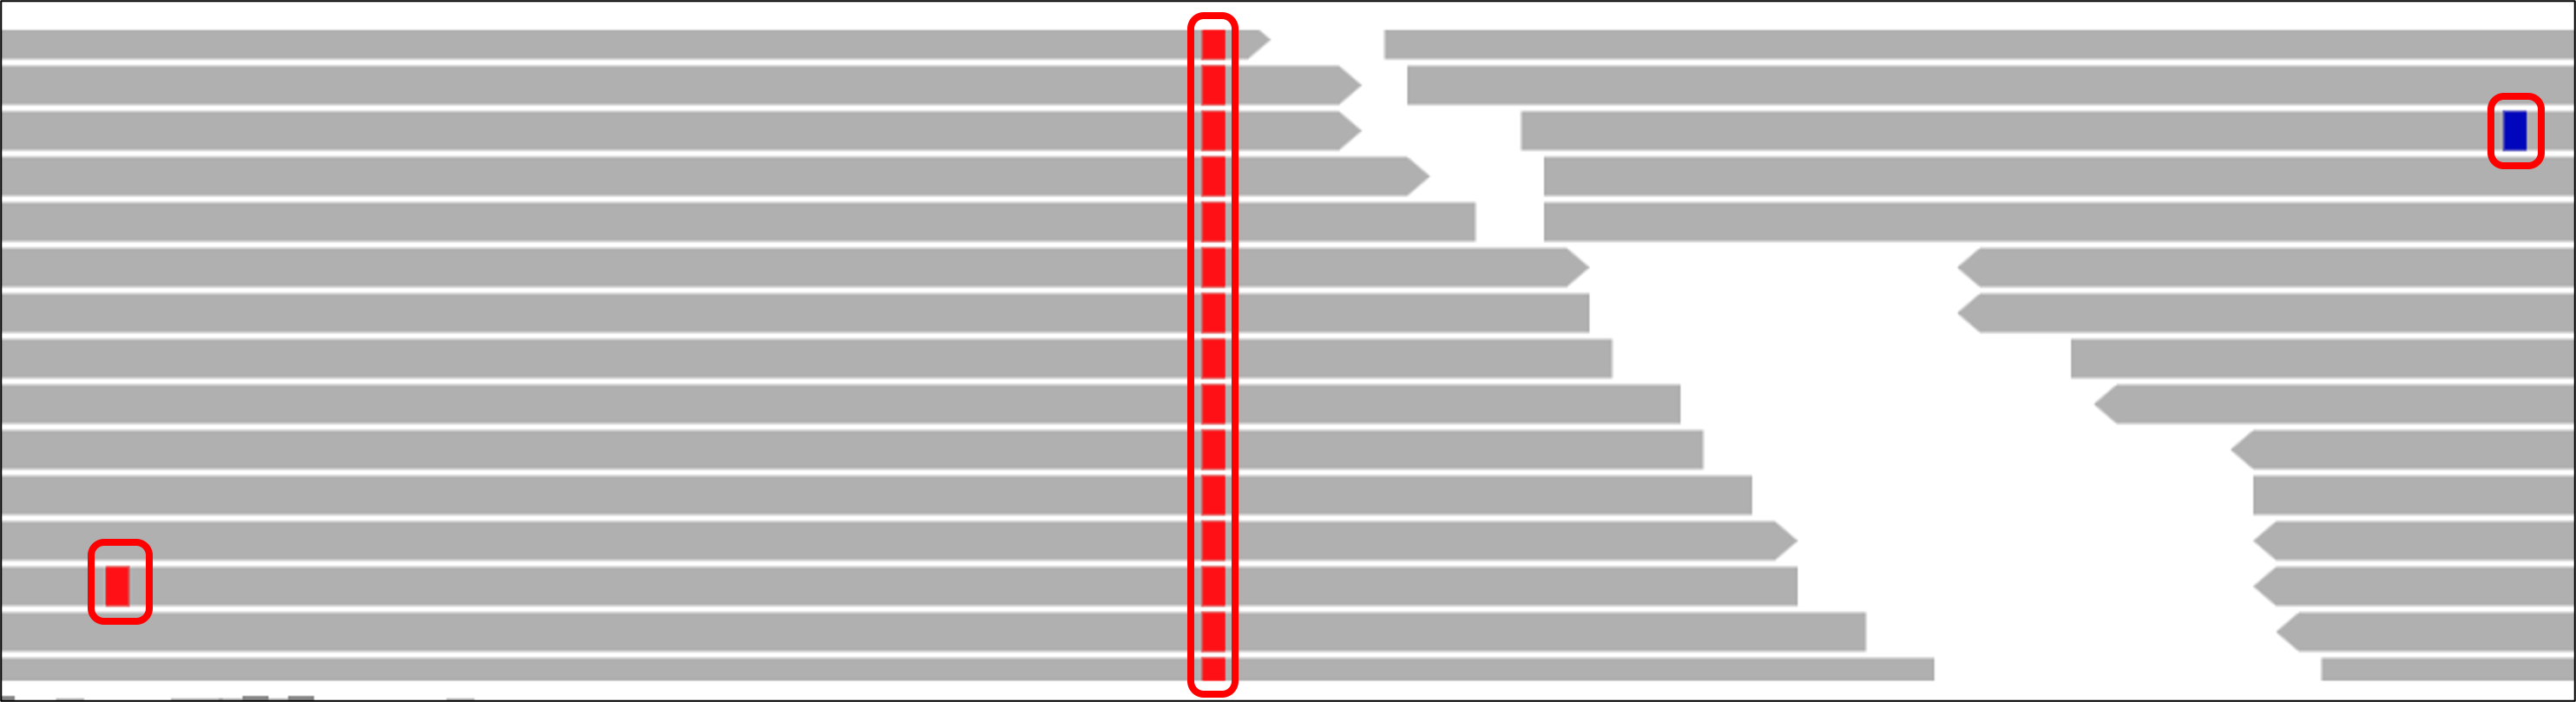
\includegraphics[width=0.5\linewidth,height=\textheight,keepaspectratio]{images/slide-35-image-1.png}

To gauge whether any sequence differences might represent germline
variants, we can examine the bases observed at each position by clicking
on a base in the mountain plot at the top of each read track.

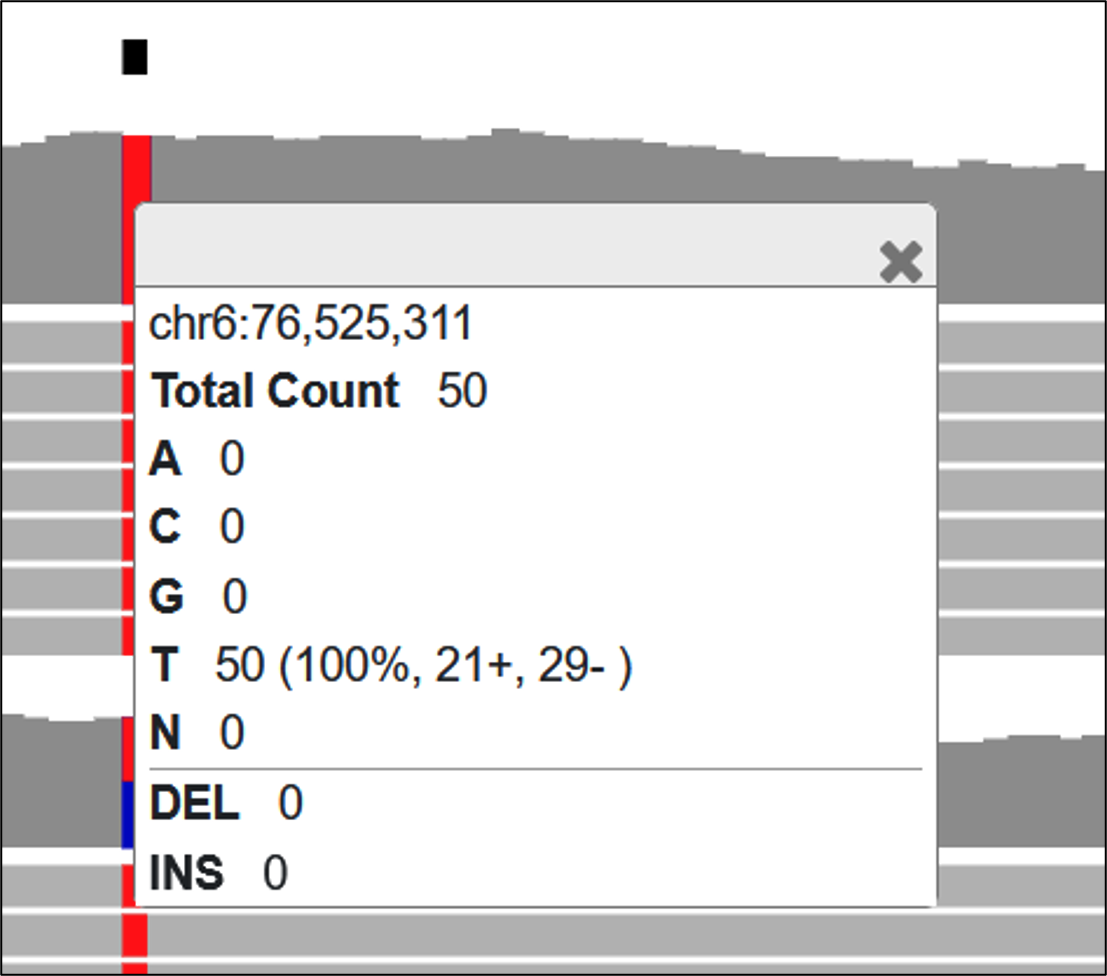
\includegraphics[width=0.5\linewidth,height=\textheight,keepaspectratio]{images/slide-36-image-1.png}

\begin{tcolorbox}[enhanced jigsaw, arc=.35mm, bottomrule=.15mm, bottomtitle=1mm, breakable, colback=white, colbacktitle=quarto-callout-tip-color!10!white, colframe=quarto-callout-tip-color-frame, coltitle=black, left=2mm, leftrule=.75mm, opacityback=0, opacitybacktitle=0.6, rightrule=.15mm, title=\textcolor{quarto-callout-tip-color}{\faLightbulb}\hspace{0.5em}{Test your understanding}, titlerule=0mm, toprule=.15mm, toptitle=1mm]

\begin{itemize}
\tightlist
\item
  What do you think is the germline genotype for NA12877 (the son) at
  position ch6:76,525,300?
\item
  What are the possible sources of the G read observed?
\end{itemize}

\end{tcolorbox}

\begin{tcolorbox}[enhanced jigsaw, arc=.35mm, bottomrule=.15mm, bottomtitle=1mm, breakable, colback=white, colbacktitle=quarto-callout-tip-color!10!white, colframe=quarto-callout-tip-color-frame, coltitle=black, left=2mm, leftrule=.75mm, opacityback=0, opacitybacktitle=0.6, rightrule=.15mm, title=\textcolor{quarto-callout-tip-color}{\faLightbulb}\hspace{0.5em}{Answer}, titlerule=0mm, toprule=.15mm, toptitle=1mm]

\begin{itemize}
\tightlist
\item
  This position appears to be homozygous A (A/A) because all the reads
  are the same
\item
  Most likely a sequencing error, but could possibly be a rare somatic
  variant
\end{itemize}

\end{tcolorbox}

Moving along slightly to position 76,525,311:

\pandocbounded{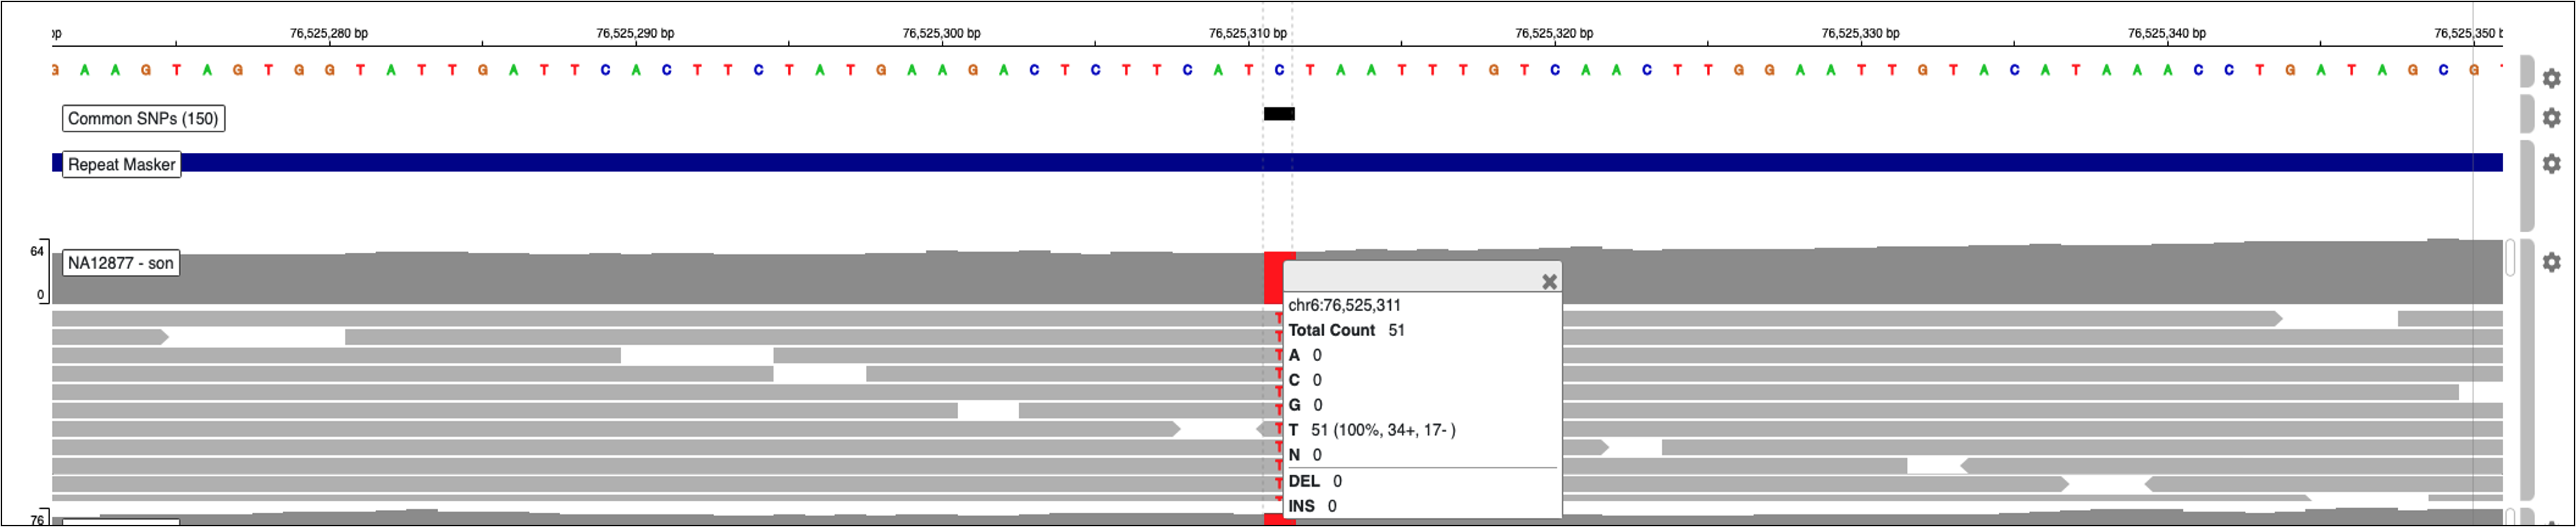
\includegraphics[keepaspectratio]{images/slide-37-image-1.png}}

\begin{tcolorbox}[enhanced jigsaw, arc=.35mm, bottomrule=.15mm, bottomtitle=1mm, breakable, colback=white, colbacktitle=quarto-callout-tip-color!10!white, colframe=quarto-callout-tip-color-frame, coltitle=black, left=2mm, leftrule=.75mm, opacityback=0, opacitybacktitle=0.6, rightrule=.15mm, title=\textcolor{quarto-callout-tip-color}{\faLightbulb}\hspace{0.5em}{Test your understanding}, titlerule=0mm, toprule=.15mm, toptitle=1mm]

\begin{itemize}
\tightlist
\item
  What is the reference sequence at position chr6:76,525,311?
\item
  What is the germline genotype at position chr6:76,525,311 for NA12877
  (the son)?
\item
  How sure are we that this is not a sequencing error?
\end{itemize}

\end{tcolorbox}

\begin{tcolorbox}[enhanced jigsaw, arc=.35mm, bottomrule=.15mm, bottomtitle=1mm, breakable, colback=white, colbacktitle=quarto-callout-tip-color!10!white, colframe=quarto-callout-tip-color-frame, coltitle=black, left=2mm, leftrule=.75mm, opacityback=0, opacitybacktitle=0.6, rightrule=.15mm, title=\textcolor{quarto-callout-tip-color}{\faLightbulb}\hspace{0.5em}{Answer}, titlerule=0mm, toprule=.15mm, toptitle=1mm]

\begin{itemize}
\tightlist
\item
  The reference sequence at position chr6:76,525,311 is \textbf{C}
\item
  The germline genotype at position chr6:76,525,311 for NA12877 is
  Homozygous T (T/T)
\item
  All 51 reads contained T at this position, making a sequencing error
  highly unlikely. The germline genotype is therefore very likely to be
  T/T
\end{itemize}

\end{tcolorbox}

Examine the reads for the other members of the trio.

\pandocbounded{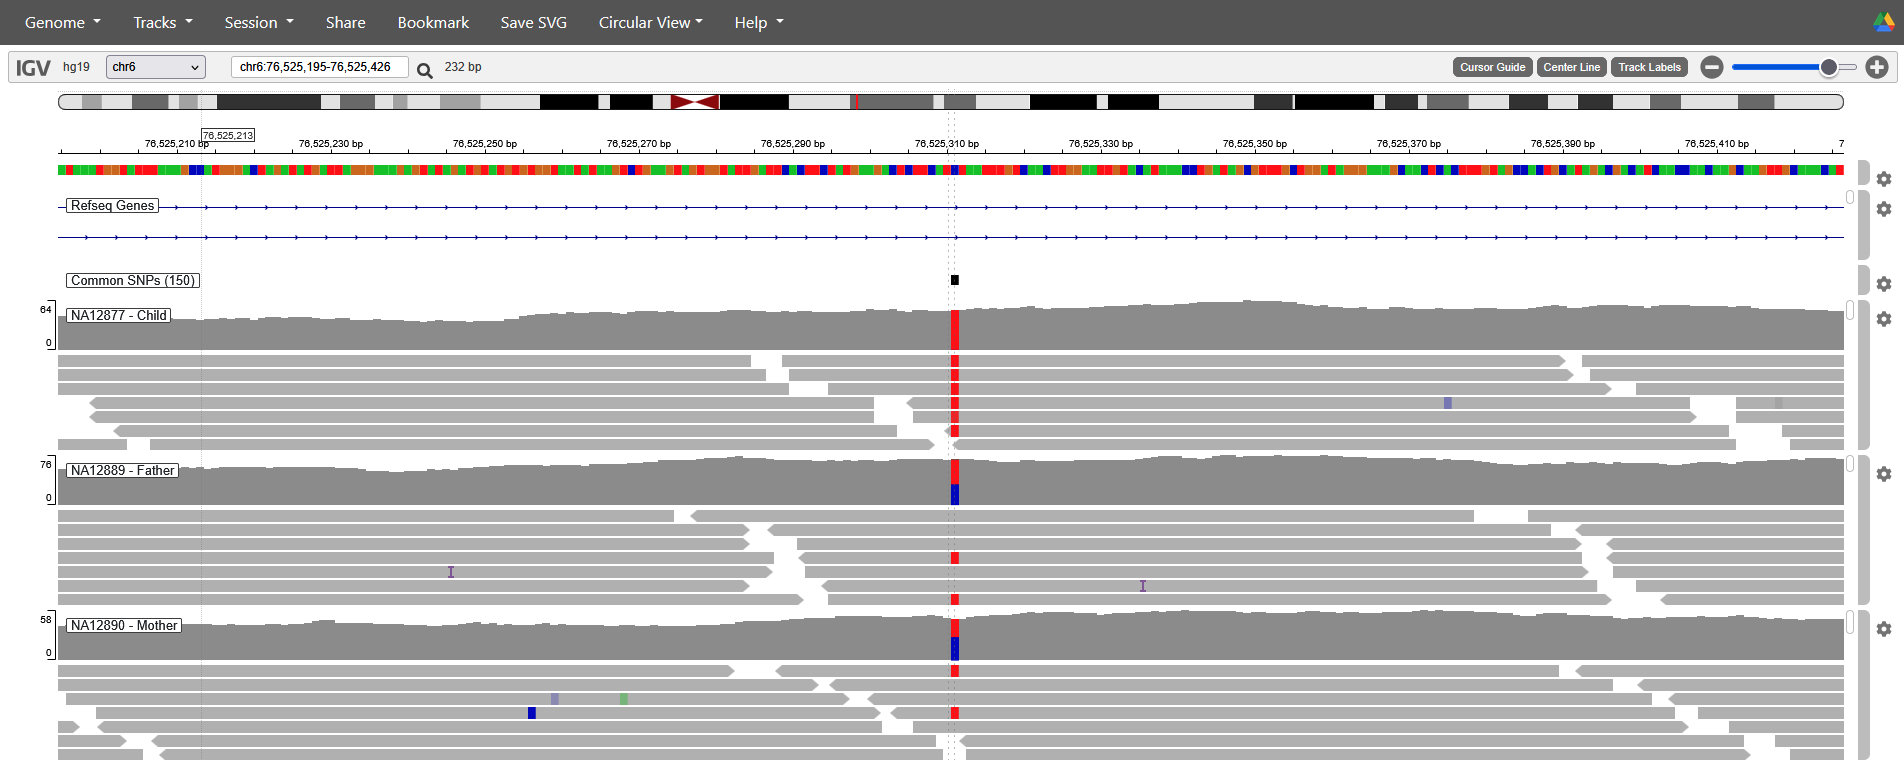
\includegraphics[keepaspectratio]{images/slide-38-image-1.png}}

\begin{tcolorbox}[enhanced jigsaw, arc=.35mm, bottomrule=.15mm, bottomtitle=1mm, breakable, colback=white, colbacktitle=quarto-callout-tip-color!10!white, colframe=quarto-callout-tip-color-frame, coltitle=black, left=2mm, leftrule=.75mm, opacityback=0, opacitybacktitle=0.6, rightrule=.15mm, title=\textcolor{quarto-callout-tip-color}{\faLightbulb}\hspace{0.5em}{Test your understanding}, titlerule=0mm, toprule=.15mm, toptitle=1mm]

\begin{itemize}
\tightlist
\item
  What are the genotypes at position chr6:76,525,311 for NA12889 and
  NA12890?
\item
  Are the predicted genotypes consistent with Mendelian expectations?
\end{itemize}

\end{tcolorbox}

\begin{tcolorbox}[enhanced jigsaw, arc=.35mm, bottomrule=.15mm, bottomtitle=1mm, breakable, colback=white, colbacktitle=quarto-callout-tip-color!10!white, colframe=quarto-callout-tip-color-frame, coltitle=black, left=2mm, leftrule=.75mm, opacityback=0, opacitybacktitle=0.6, rightrule=.15mm, title=\textcolor{quarto-callout-tip-color}{\faLightbulb}\hspace{0.5em}{Answer}, titlerule=0mm, toprule=.15mm, toptitle=1mm]

\begin{itemize}
\tightlist
\item
  Both parents are heterozygous T/C
\item
  The pattern does fit with Mendelian expectations: father T/C, mother
  T/C and son T/T suggest the son inherited a T from each parent
\end{itemize}

\end{tcolorbox}

By clicking on the feature in the Common SNPs track we can see that this
is a known SNP and gain additional information:

\pandocbounded{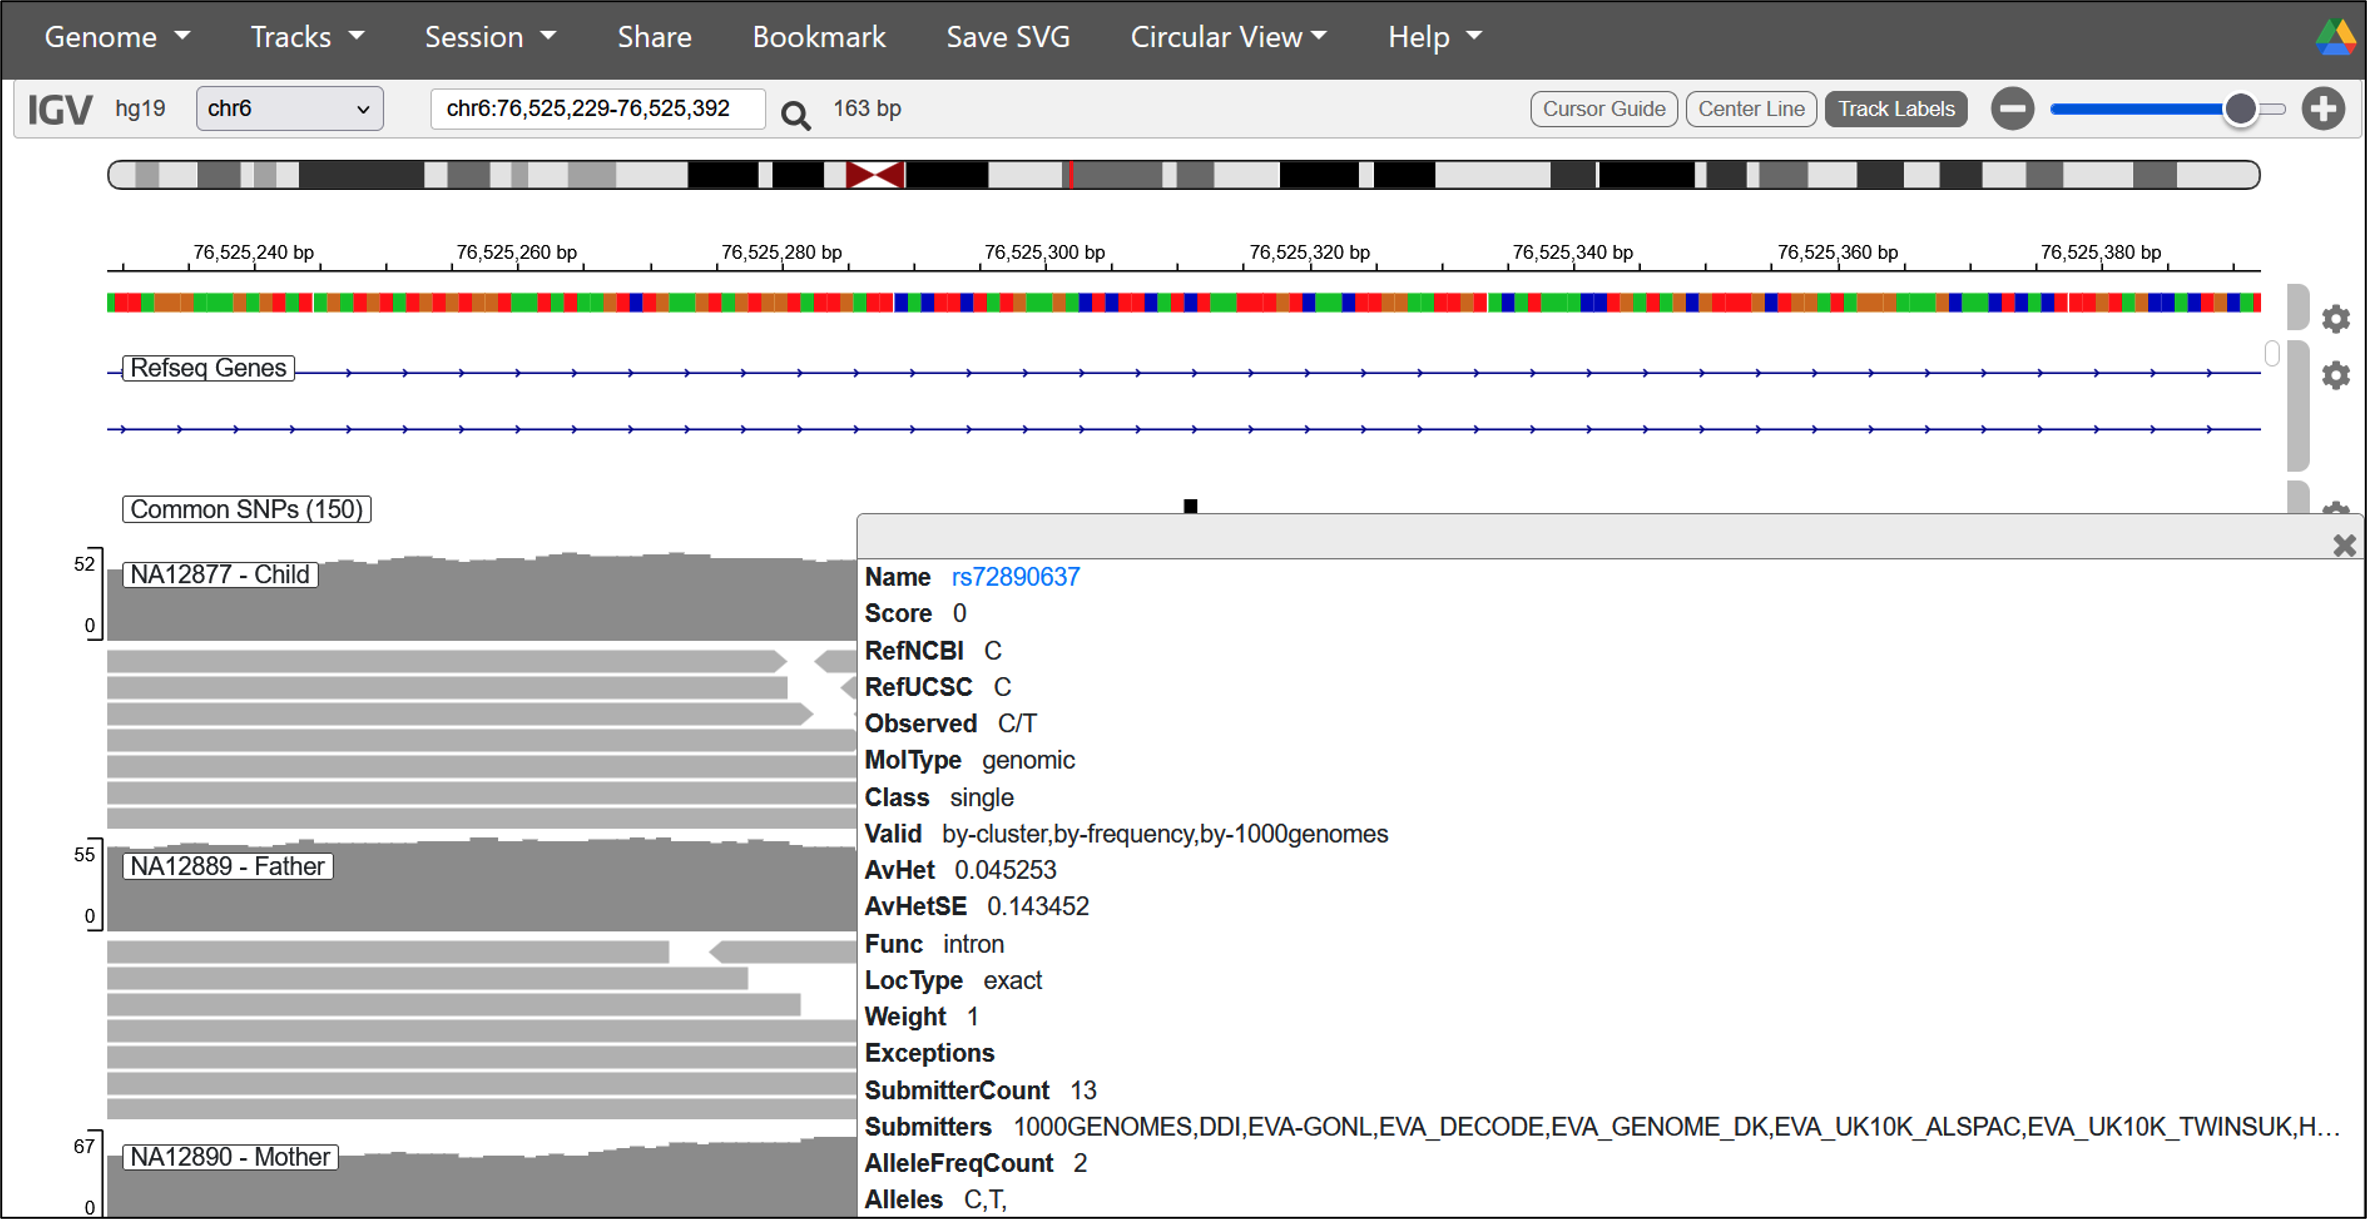
\includegraphics[keepaspectratio]{images/slide-39-image-1.png}}

\begin{tcolorbox}[enhanced jigsaw, arc=.35mm, bottomrule=.15mm, bottomtitle=1mm, breakable, colback=white, colbacktitle=quarto-callout-tip-color!10!white, colframe=quarto-callout-tip-color-frame, coltitle=black, left=2mm, leftrule=.75mm, opacityback=0, opacitybacktitle=0.6, rightrule=.15mm, title=\textcolor{quarto-callout-tip-color}{\faLightbulb}\hspace{0.5em}{Test your understanding}, titlerule=0mm, toprule=.15mm, toptitle=1mm]

\begin{itemize}
\tightlist
\item
  What is the identifier (name) of the SNP at this position?
\item
  What is the minor allele frequency (MAF)?
\end{itemize}

\end{tcolorbox}

\begin{tcolorbox}[enhanced jigsaw, arc=.35mm, bottomrule=.15mm, bottomtitle=1mm, breakable, colback=white, colbacktitle=quarto-callout-tip-color!10!white, colframe=quarto-callout-tip-color-frame, coltitle=black, left=2mm, leftrule=.75mm, opacityback=0, opacitybacktitle=0.6, rightrule=.15mm, title=\textcolor{quarto-callout-tip-color}{\faLightbulb}\hspace{0.5em}{Answer}, titlerule=0mm, toprule=.15mm, toptitle=1mm]

\begin{itemize}
\tightlist
\item
  The SNP identifier is rs72890637
\item
  The MAF is 0.023
\end{itemize}

\end{tcolorbox}

\bookmarksetup{startatroot}

\chapter{Investigate variants using
Ensembl}\label{investigate-variants-using-ensembl}

We can find out even more about this SNP using the
\href{https://www.ensembl.org/search}{Ensembl database}. Enter the SNP
identifier (rs72890637) into the Ensembl search box (If Ensembl search
is down, use the
\href{https://www.ensembl.org/feature-explorer/GCA_000001405.29/variant:6:75815594:rs72890637?allele=0}{direct
link to the SNP})

\pandocbounded{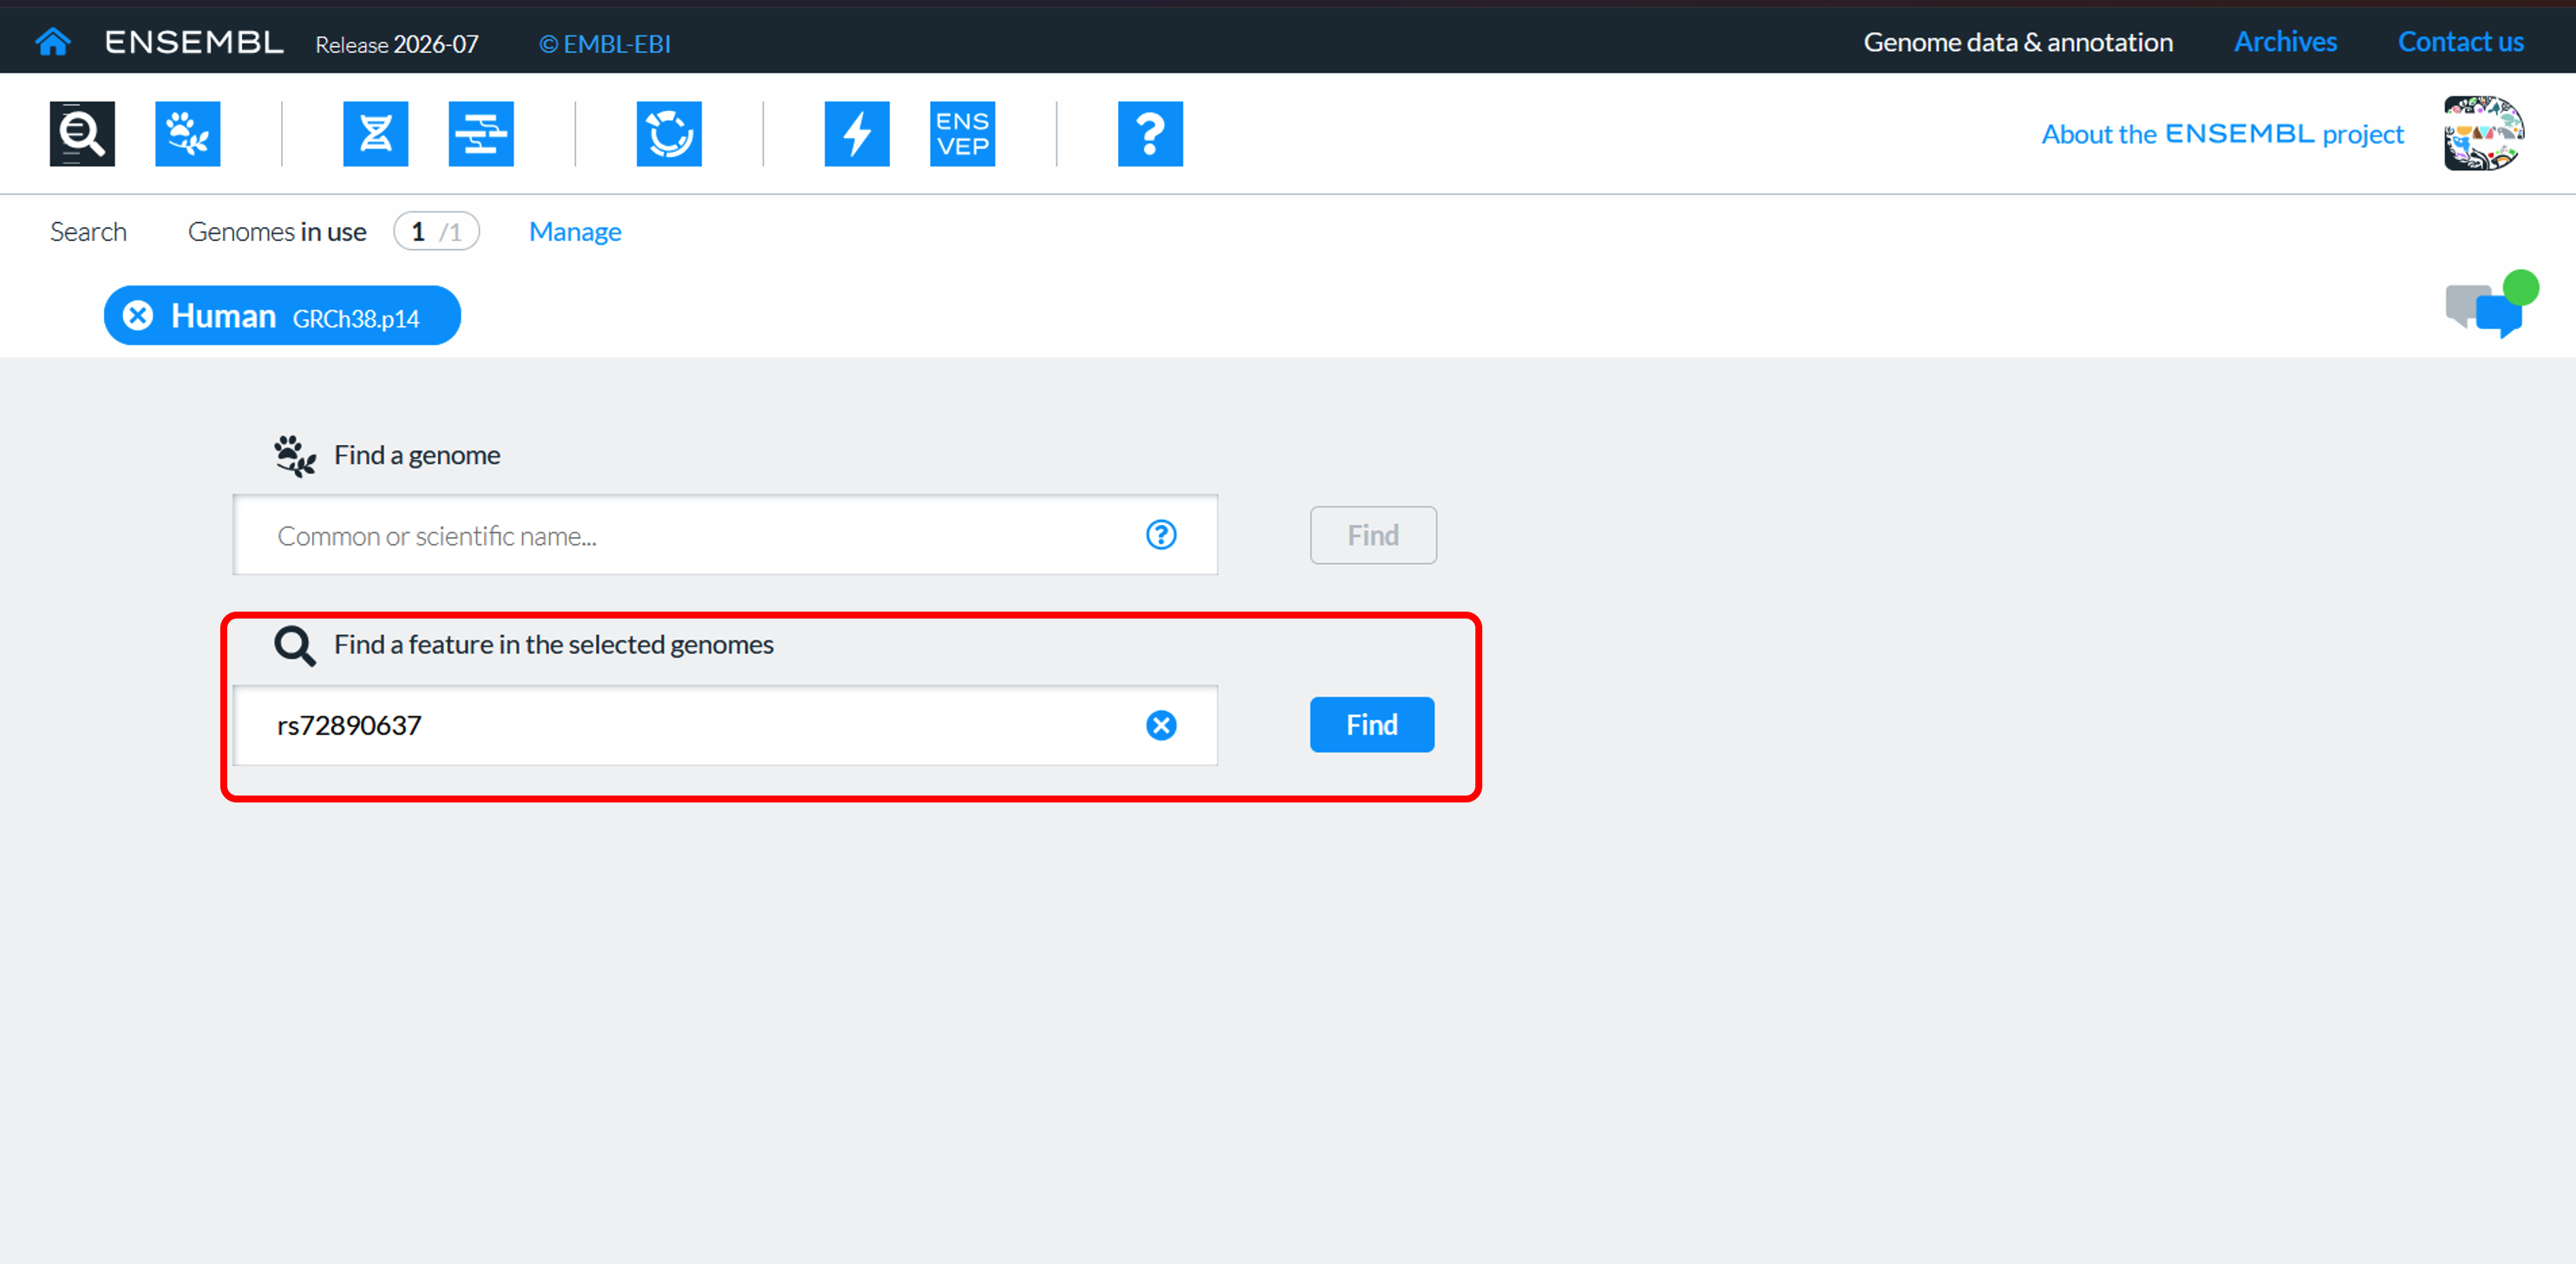
\includegraphics[keepaspectratio]{images/slide-40-image-1.png}}

Then click on the link in the Ensembl \textbf{Feature explorer} search
results.

\pandocbounded{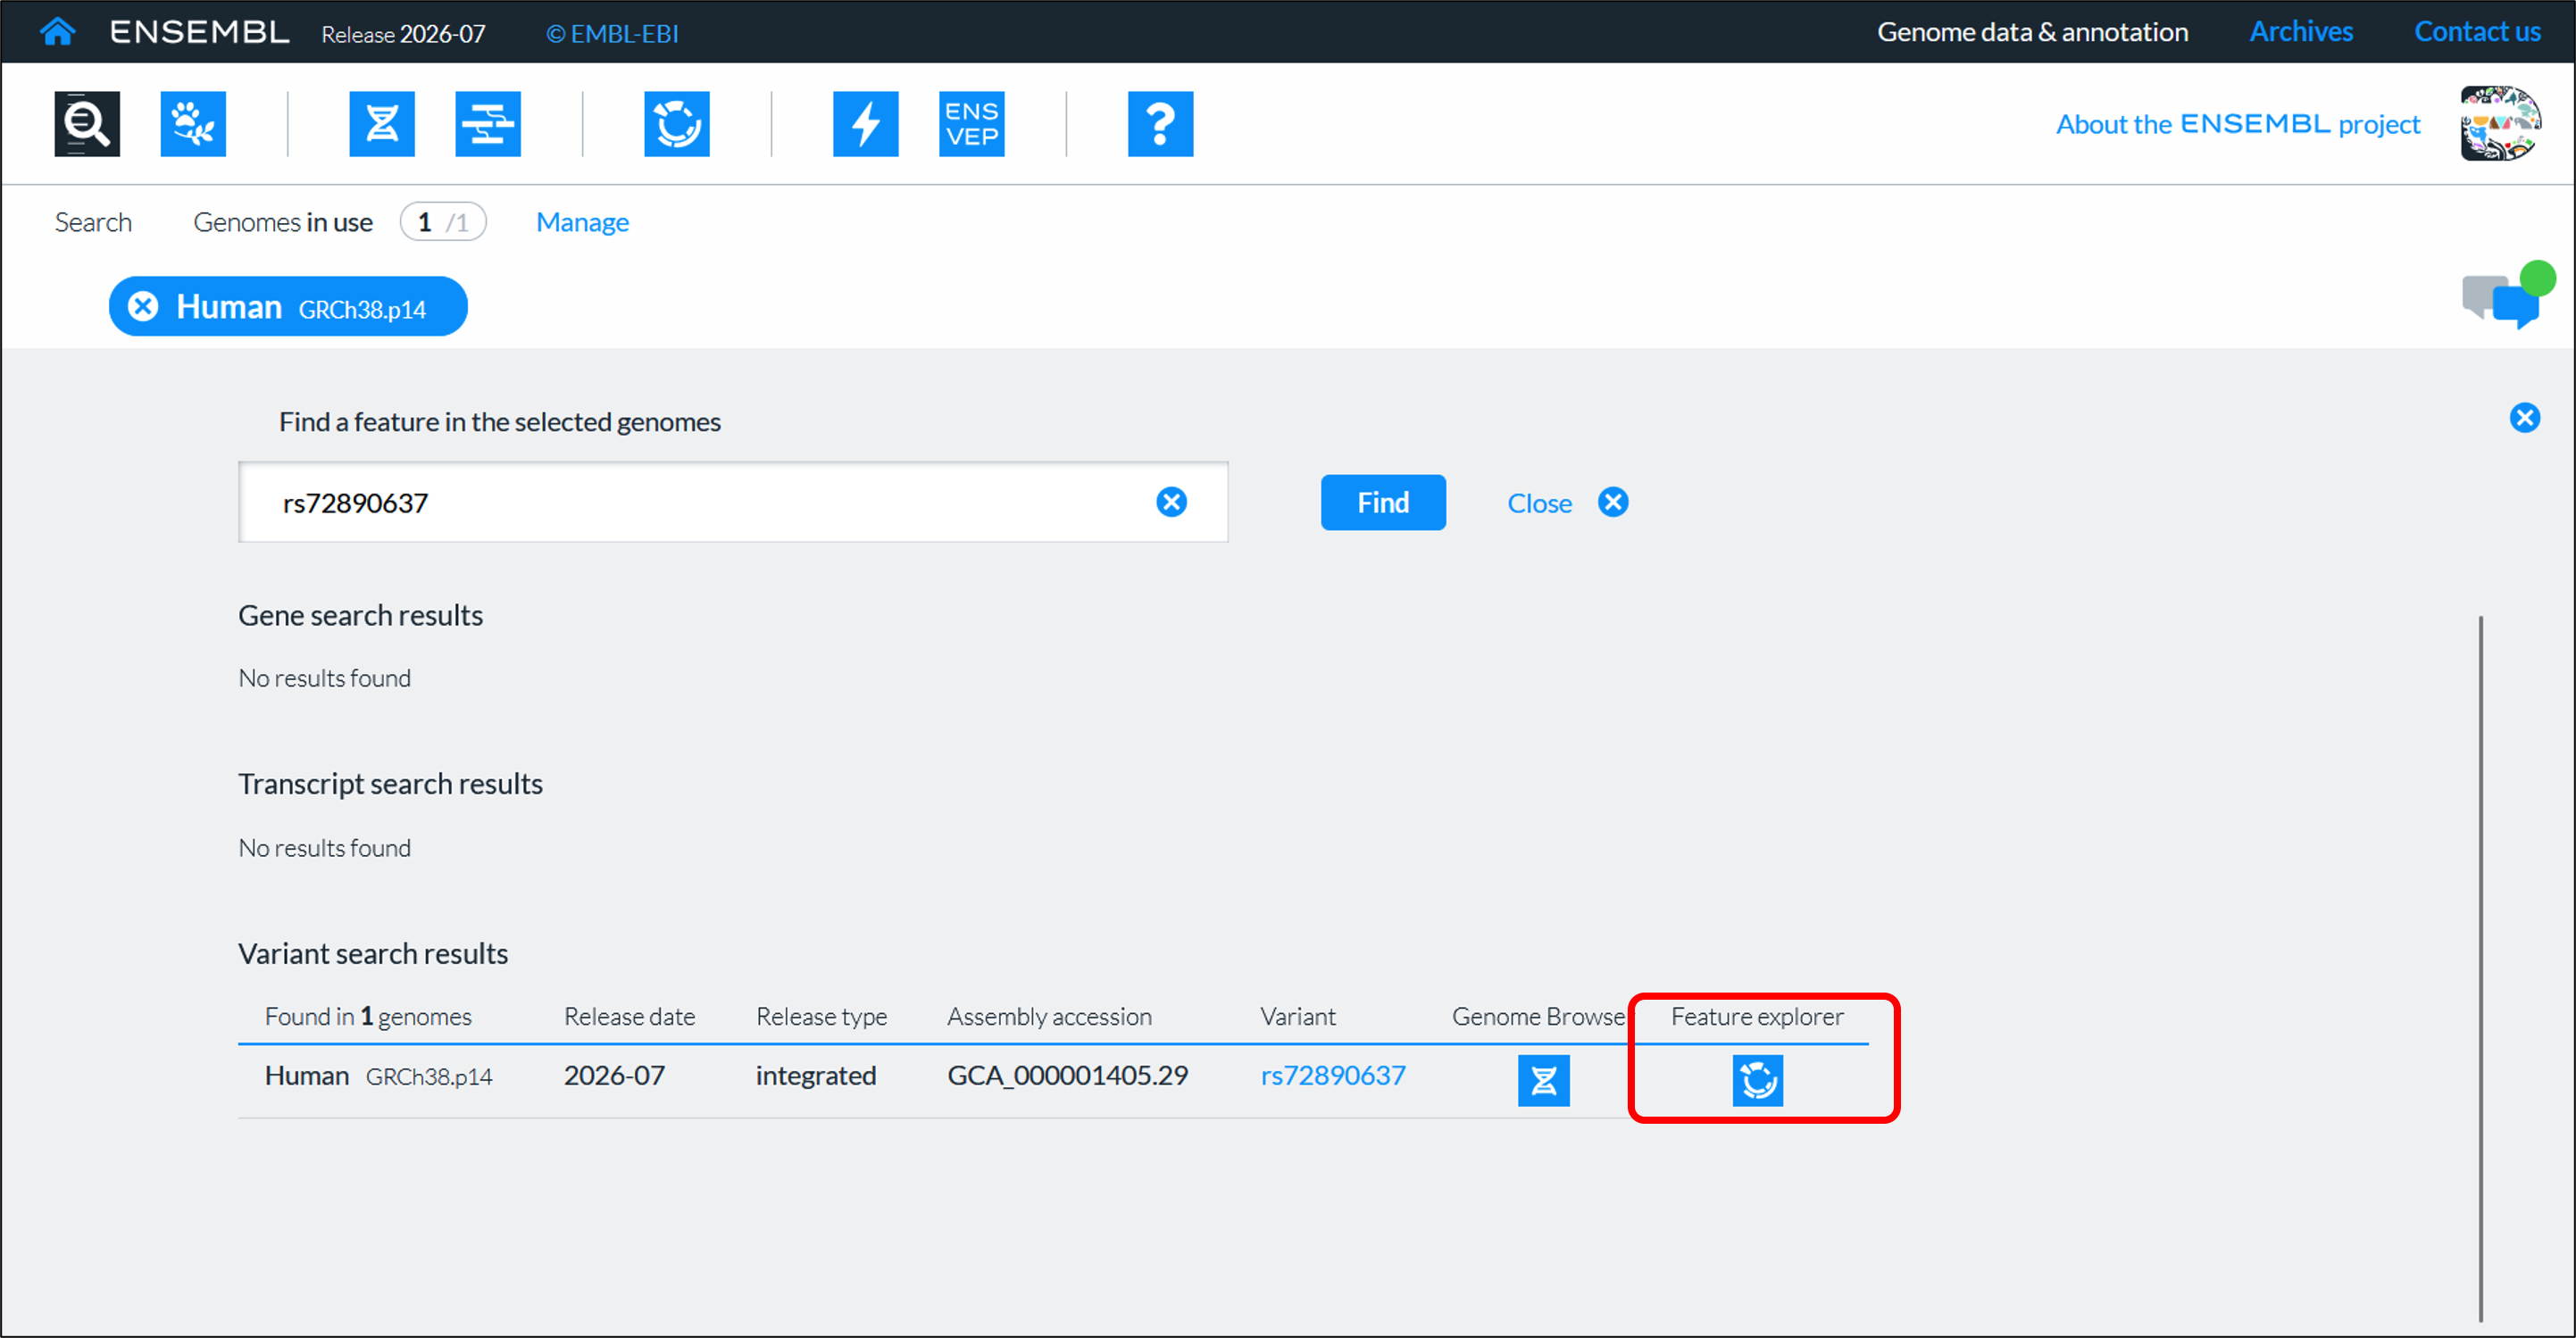
\includegraphics[keepaspectratio]{images/slide-41-image-1.png}}

There are then links to various pieces of data about the SNP. Click on
the \textbf{Allele Frequency} link.

\pandocbounded{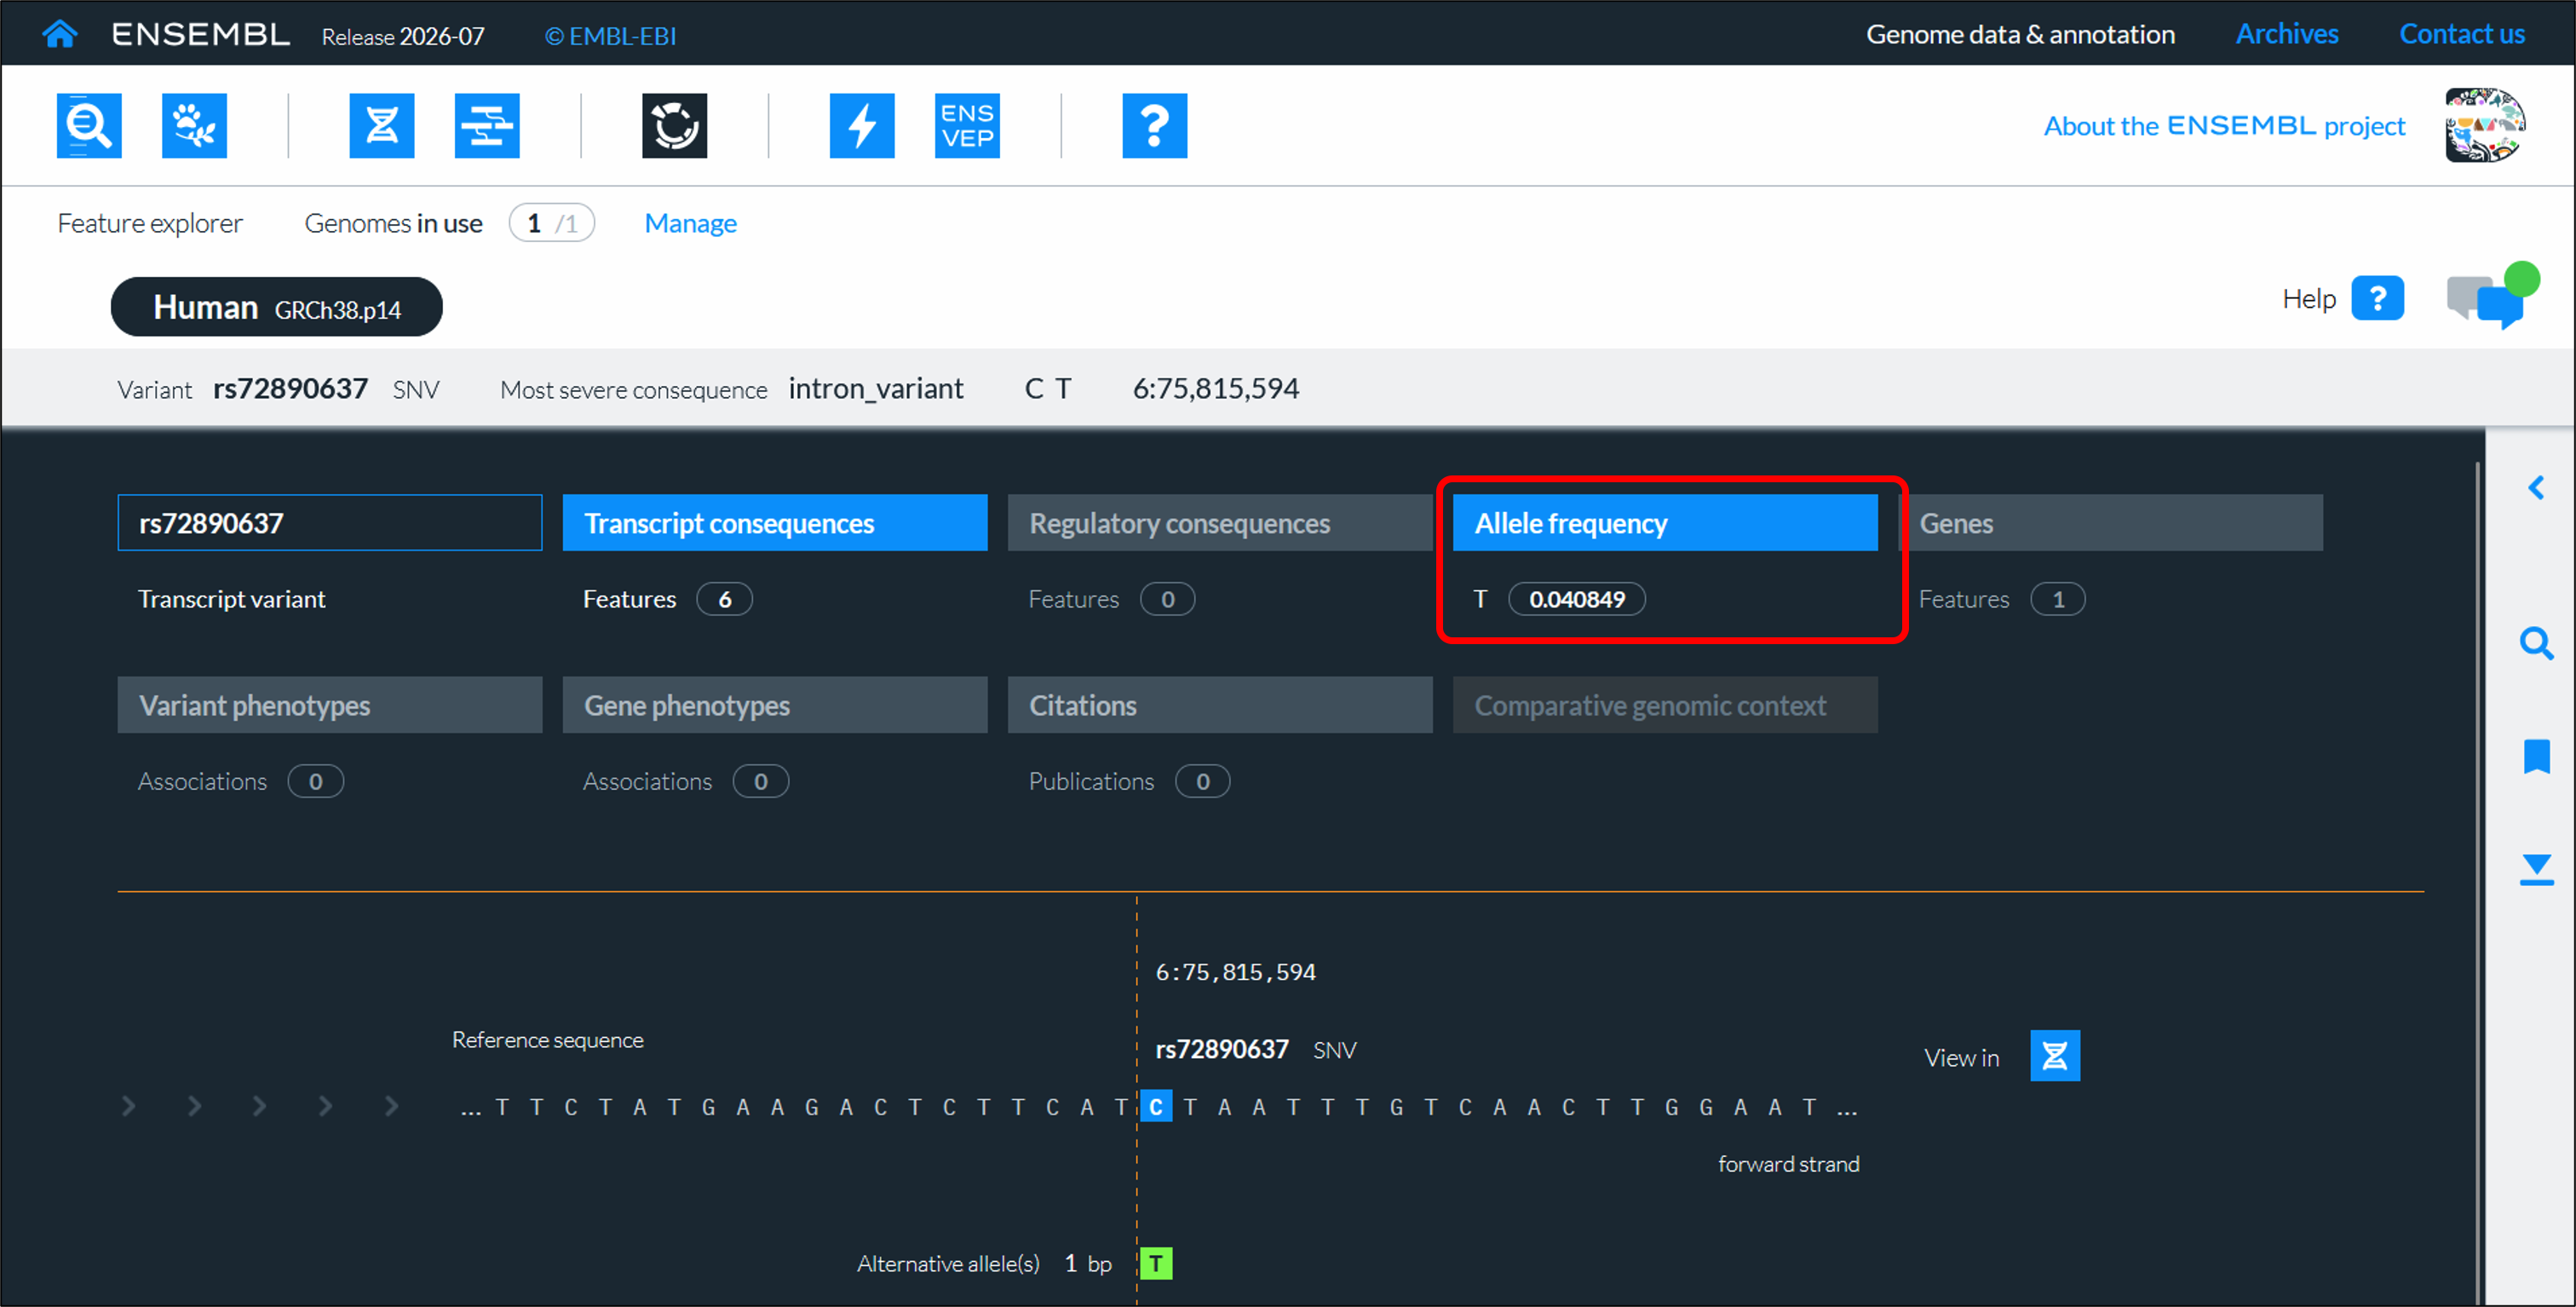
\includegraphics[keepaspectratio]{images/slide-42-image-1.png}}

\begin{tcolorbox}[enhanced jigsaw, arc=.35mm, bottomrule=.15mm, bottomtitle=1mm, breakable, colback=white, colbacktitle=quarto-callout-tip-color!10!white, colframe=quarto-callout-tip-color-frame, coltitle=black, left=2mm, leftrule=.75mm, opacityback=0, opacitybacktitle=0.6, rightrule=.15mm, title=\textcolor{quarto-callout-tip-color}{\faLightbulb}\hspace{0.5em}{Test your understanding}, titlerule=0mm, toprule=.15mm, toptitle=1mm]

\begin{itemize}
\tightlist
\item
  What is the minor allele frequency in Finland? (you may have to expand
  the gnomAD genomes v4.1 dataset)
\item
  How does that compare to the wider, non-Finnish European population?
\end{itemize}

\end{tcolorbox}

\begin{tcolorbox}[enhanced jigsaw, arc=.35mm, bottomrule=.15mm, bottomtitle=1mm, breakable, colback=white, colbacktitle=quarto-callout-tip-color!10!white, colframe=quarto-callout-tip-color-frame, coltitle=black, left=2mm, leftrule=.75mm, opacityback=0, opacitybacktitle=0.6, rightrule=.15mm, title=\textcolor{quarto-callout-tip-color}{\faLightbulb}\hspace{0.5em}{Answer}, titlerule=0mm, toprule=.15mm, toptitle=1mm]

\begin{itemize}
\tightlist
\item
  The MAF for Finnish Europeans is 9\%
\item
  The wider European population MAF is 6\%. Finland often differs from
  other European populations because of a phenomenon called the Finnish
  founder effect that has emerged because of a small founder population,
  various bottlenecks, geographic isolation and low immigration.
\end{itemize}

\end{tcolorbox}

\bookmarksetup{startatroot}

\chapter{Genotypes, inheritance and
haplotypes}\label{genotypes-inheritance-and-haplotypes}

Let's look at a few more variants. To start with, we'll focus on
rs1280055. We can jump straight to this SNP by typing its ID into the
IGV search bar.

\pandocbounded{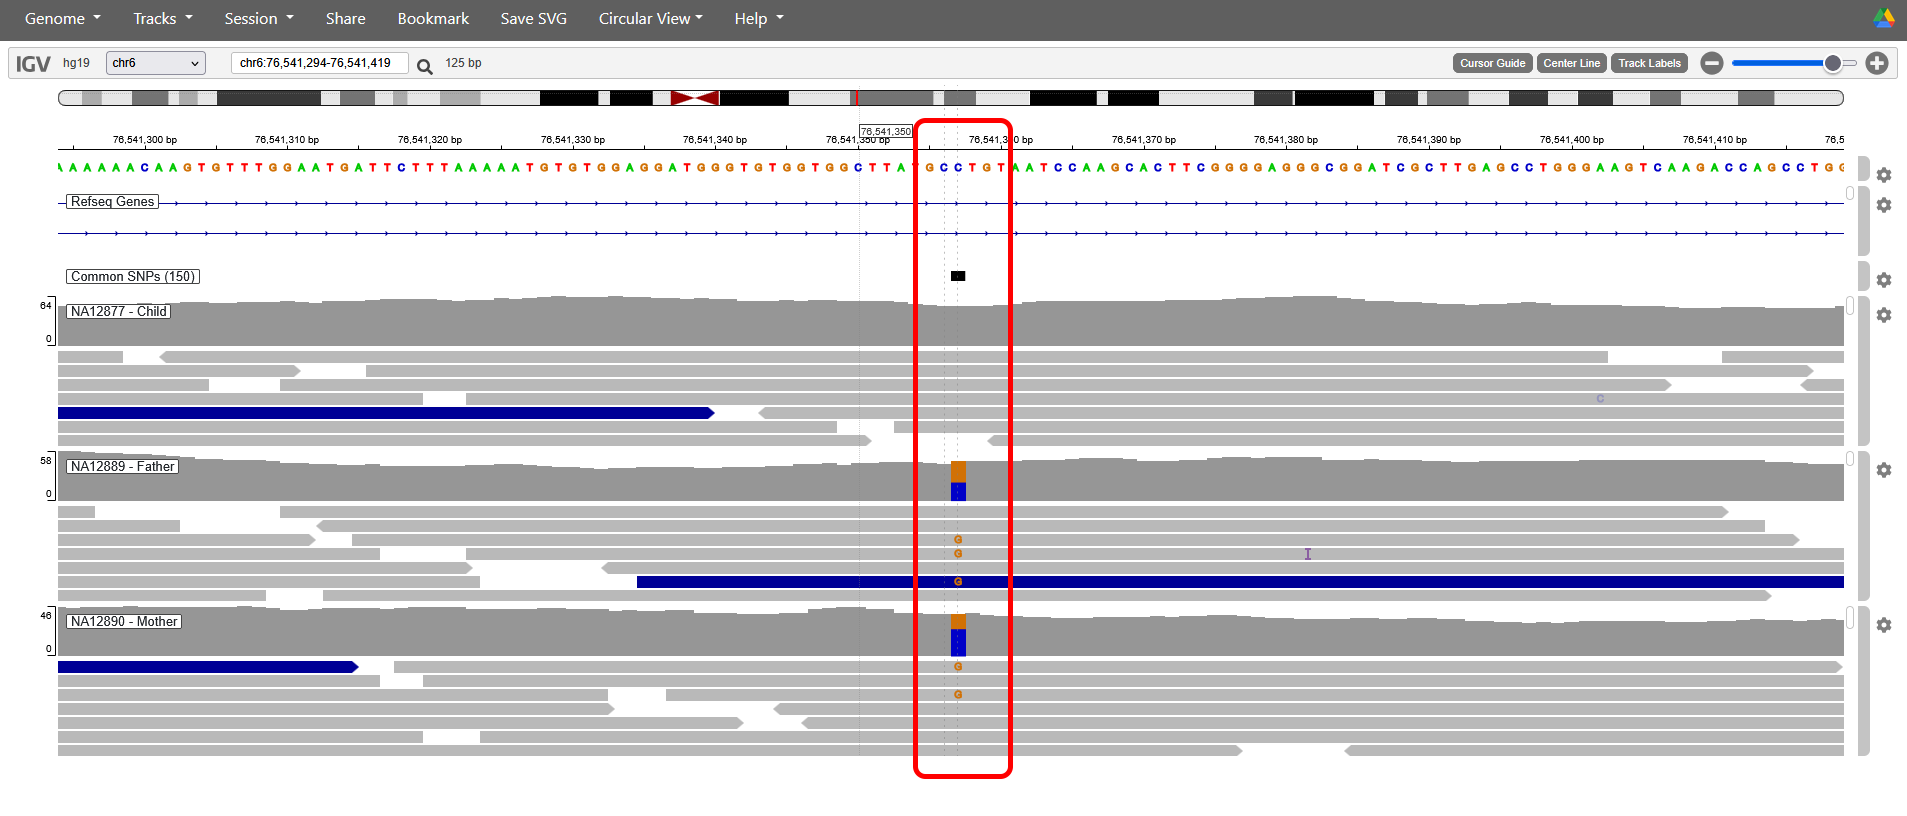
\includegraphics[keepaspectratio]{images/slide-44-image-1.png}}

\begin{tcolorbox}[enhanced jigsaw, arc=.35mm, bottomrule=.15mm, bottomtitle=1mm, breakable, colback=white, colbacktitle=quarto-callout-tip-color!10!white, colframe=quarto-callout-tip-color-frame, coltitle=black, left=2mm, leftrule=.75mm, opacityback=0, opacitybacktitle=0.6, rightrule=.15mm, title=\textcolor{quarto-callout-tip-color}{\faLightbulb}\hspace{0.5em}{Test your understanding}, titlerule=0mm, toprule=.15mm, toptitle=1mm]

\begin{itemize}
\tightlist
\item
  What are the genotypes at rs1280055 for NA12877, NA12889 and NA12890?
\item
  Are they consistent with Mendelian inheritance patterns?
\end{itemize}

\end{tcolorbox}

\begin{tcolorbox}[enhanced jigsaw, arc=.35mm, bottomrule=.15mm, bottomtitle=1mm, breakable, colback=white, colbacktitle=quarto-callout-tip-color!10!white, colframe=quarto-callout-tip-color-frame, coltitle=black, left=2mm, leftrule=.75mm, opacityback=0, opacitybacktitle=0.6, rightrule=.15mm, title=\textcolor{quarto-callout-tip-color}{\faLightbulb}\hspace{0.5em}{Answer}, titlerule=0mm, toprule=.15mm, toptitle=1mm]

\begin{itemize}
\tightlist
\item
  The genotypes are C/C for NA12877 (child), G/C for NA12889 (father)
  and G/C for NA12890 (mother)
\item
  These are consistent with Mendelian inheritance and the child has
  inherited a C allele from each heterozygous parent
\end{itemize}

\end{tcolorbox}

Scroll along a few hundred bases to the right and you should find
another SNP - rs1280056.

\pandocbounded{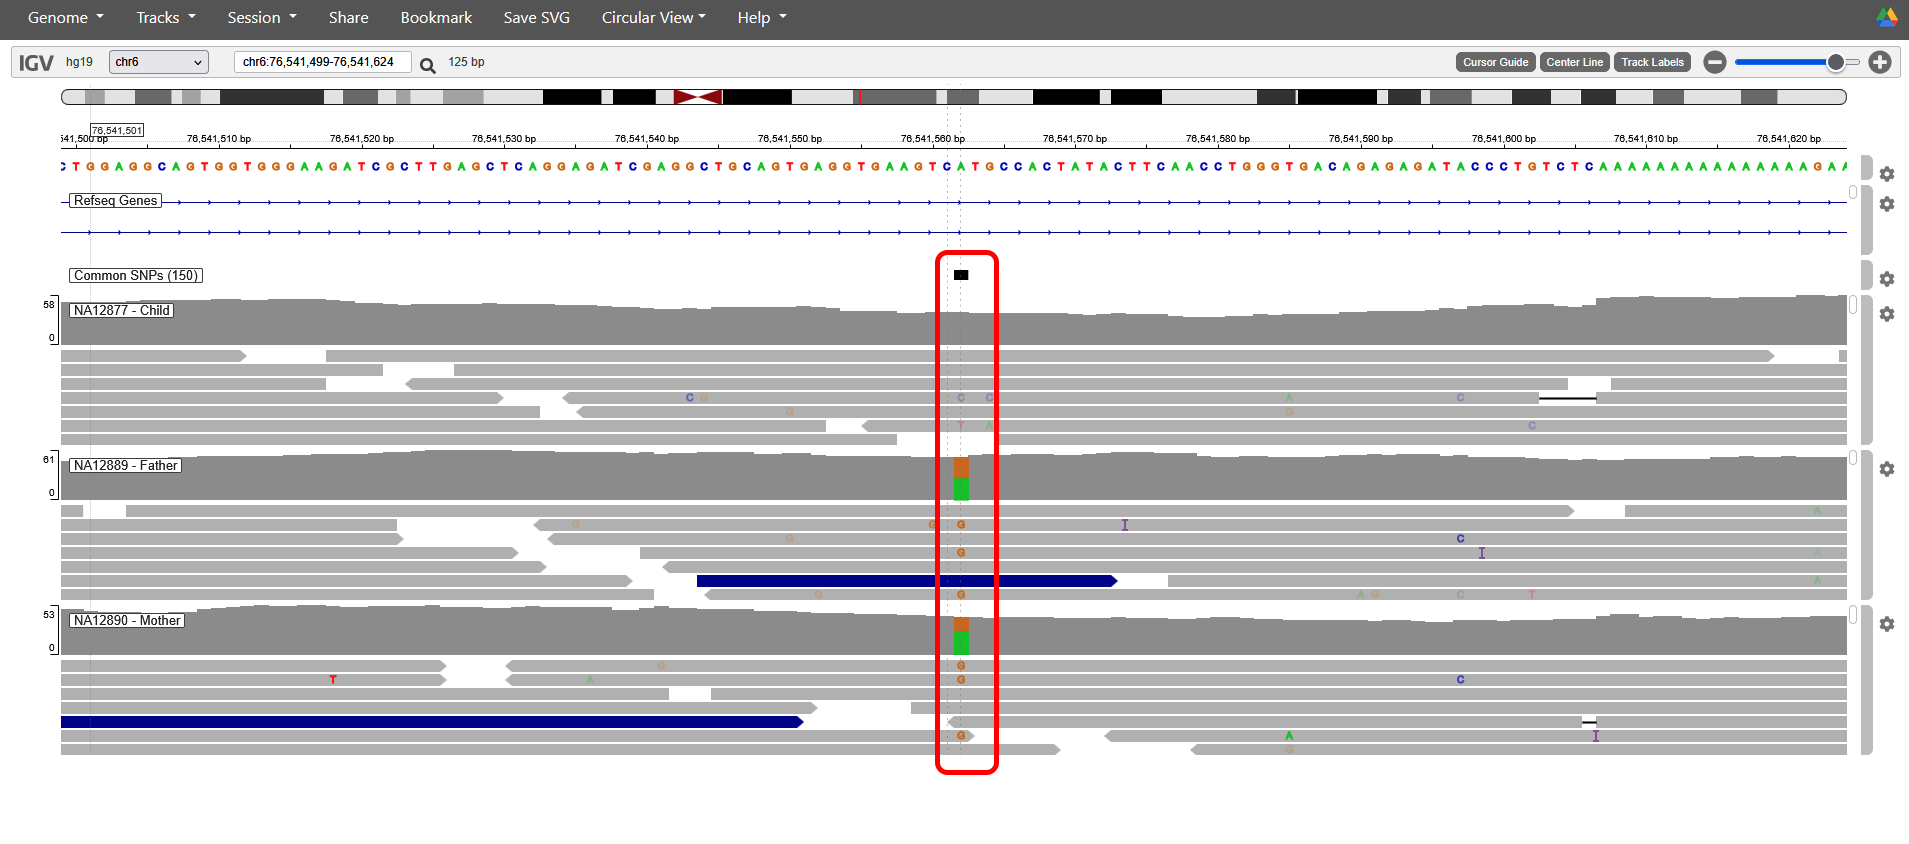
\includegraphics[keepaspectratio]{images/slide-45-image-1.png}}

\begin{tcolorbox}[enhanced jigsaw, arc=.35mm, bottomrule=.15mm, bottomtitle=1mm, breakable, colback=white, colbacktitle=quarto-callout-tip-color!10!white, colframe=quarto-callout-tip-color-frame, coltitle=black, left=2mm, leftrule=.75mm, opacityback=0, opacitybacktitle=0.6, rightrule=.15mm, title=\textcolor{quarto-callout-tip-color}{\faLightbulb}\hspace{0.5em}{Test your understanding}, titlerule=0mm, toprule=.15mm, toptitle=1mm]

\begin{itemize}
\tightlist
\item
  What are the genotypes at rs1280056 for NA12877, NA12889 and NA12890?
\end{itemize}

\end{tcolorbox}

\begin{tcolorbox}[enhanced jigsaw, arc=.35mm, bottomrule=.15mm, bottomtitle=1mm, breakable, colback=white, colbacktitle=quarto-callout-tip-color!10!white, colframe=quarto-callout-tip-color-frame, coltitle=black, left=2mm, leftrule=.75mm, opacityback=0, opacitybacktitle=0.6, rightrule=.15mm, title=\textcolor{quarto-callout-tip-color}{\faLightbulb}\hspace{0.5em}{Answer}, titlerule=0mm, toprule=.15mm, toptitle=1mm]

The genotypes are A/A for NA12877 (child), A/G for NA12889 (father) and
A/G for NA12890 (mother)

\end{tcolorbox}

To determine which variants have been inherited together on the same
chromosome, and hence which parents they likely came from, we can
`phase' the sequence to determine haplotypes. In the example below, a G
at rs1280055 is always found with a G in rs1280056 in mate pairs that
cover both SNPs. Conversely, a C in rs1280055 is always found with an A
in rs1280056. This allows us to infer the haplotype for the sample.

\pandocbounded{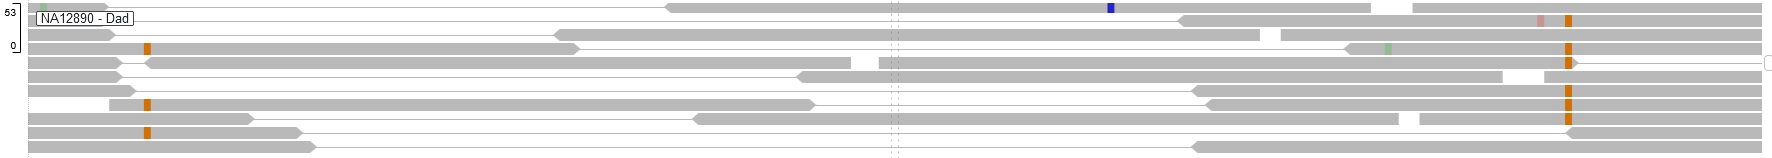
\includegraphics[keepaspectratio]{images/slide-47-image-1.png}}

By using paired reads, we can look at much longer sequence distances
than the 100 bp length of each individual read.

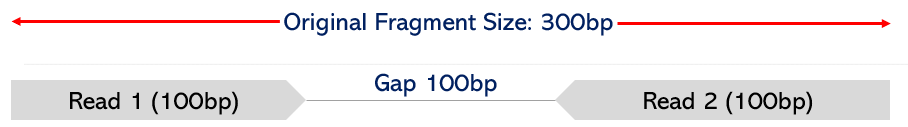
\includegraphics[width=0.5\linewidth,height=\textheight,keepaspectratio]{images/pairedexample.png}

\begin{tcolorbox}[enhanced jigsaw, arc=.35mm, bottomrule=.15mm, bottomtitle=1mm, breakable, colback=white, colbacktitle=quarto-callout-tip-color!10!white, colframe=quarto-callout-tip-color-frame, coltitle=black, left=2mm, leftrule=.75mm, opacityback=0, opacitybacktitle=0.6, rightrule=.15mm, title=\textcolor{quarto-callout-tip-color}{\faLightbulb}\hspace{0.5em}{Tip}, titlerule=0mm, toprule=.15mm, toptitle=1mm]

To help, we can use ``view as pairs'' in the parents to look for direct
physical evidence of the parental haplotypes. This setting adds a line
between read-pairs in the sequencing data, allowing us to see sequence
that comes from the same fragment and originated from a single physical
position in the genome.

\pandocbounded{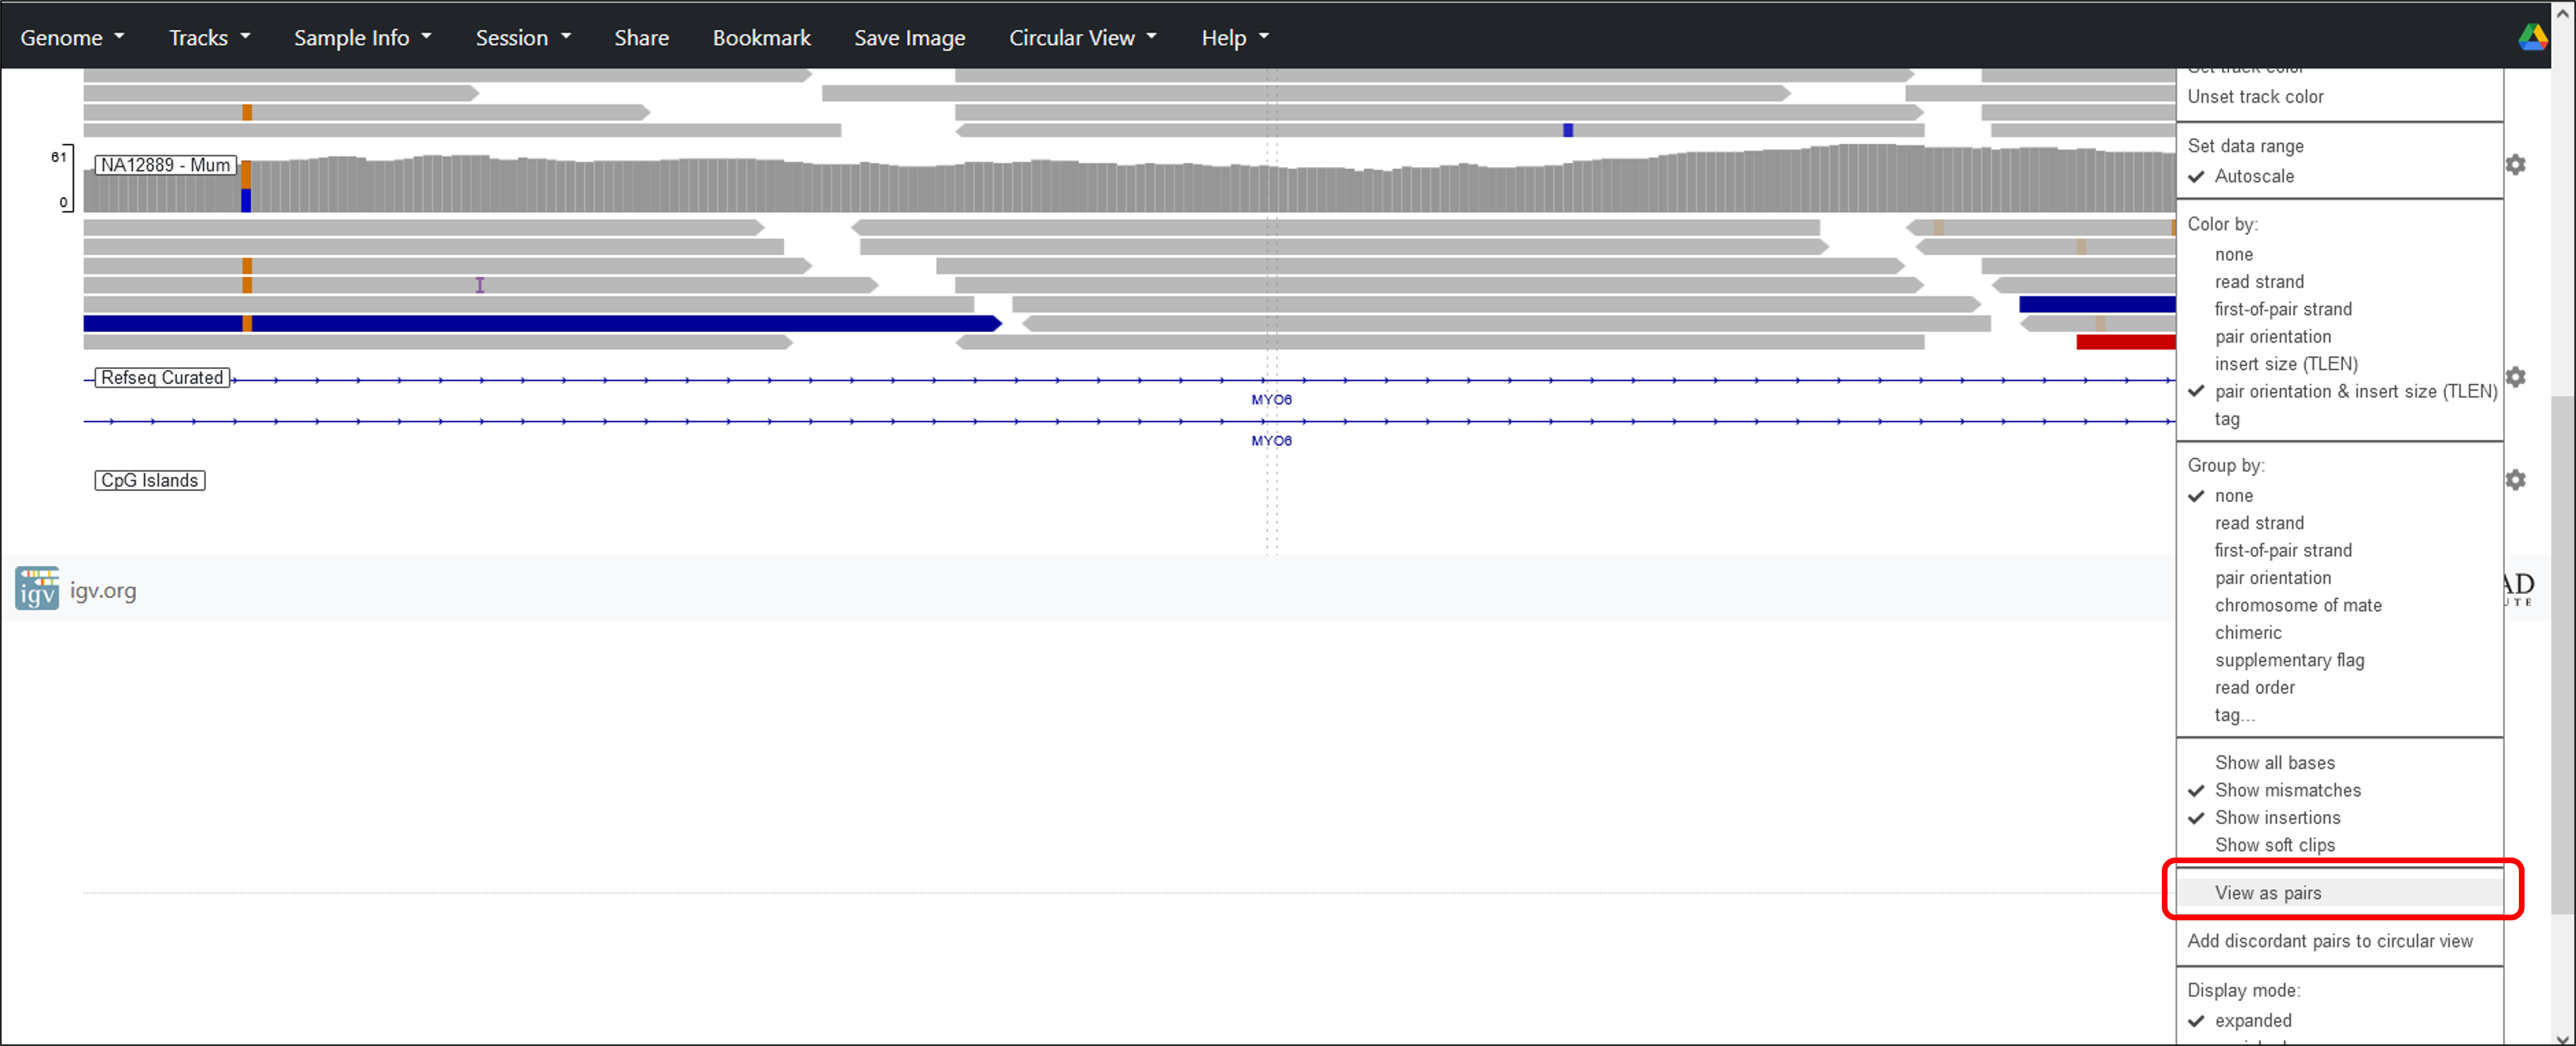
\includegraphics[keepaspectratio]{images/slide-48-image-1.png}}

\end{tcolorbox}

\begin{tcolorbox}[enhanced jigsaw, arc=.35mm, bottomrule=.15mm, bottomtitle=1mm, breakable, colback=white, colbacktitle=quarto-callout-tip-color!10!white, colframe=quarto-callout-tip-color-frame, coltitle=black, left=2mm, leftrule=.75mm, opacityback=0, opacitybacktitle=0.6, rightrule=.15mm, title=\textcolor{quarto-callout-tip-color}{\faLightbulb}\hspace{0.5em}{Test your understanding}, titlerule=0mm, toprule=.15mm, toptitle=1mm]

Use the family data and any read-pairs to phase the variants in the
table and determine the haplotypes for rs1280056 and rs1280055 in
NA12877, NA12889 and NA12890 (Don't forget to scroll up and down to view
more reads). You may have to zoom to get both SNPs on screen at the same
time.

\begin{longtable}[]{@{}
  >{\raggedright\arraybackslash}p{(\linewidth - 6\tabcolsep) * \real{0.2105}}
  >{\raggedright\arraybackslash}p{(\linewidth - 6\tabcolsep) * \real{0.2105}}
  >{\centering\arraybackslash}p{(\linewidth - 6\tabcolsep) * \real{0.2895}}
  >{\centering\arraybackslash}p{(\linewidth - 6\tabcolsep) * \real{0.2895}}@{}}
\caption{Genotypes and inferred haplotypes at rs1280056 and
rs1280055.}\label{tbl-family-haplotypes}\tabularnewline
\toprule\noalign{}
\begin{minipage}[b]{\linewidth}\raggedright
Sample
\end{minipage} & \begin{minipage}[b]{\linewidth}\raggedright
Result
\end{minipage} & \begin{minipage}[b]{\linewidth}\centering
rs1280056
\end{minipage} & \begin{minipage}[b]{\linewidth}\centering
rs1280055
\end{minipage} \\
\midrule\noalign{}
\endfirsthead
\toprule\noalign{}
\begin{minipage}[b]{\linewidth}\raggedright
Sample
\end{minipage} & \begin{minipage}[b]{\linewidth}\raggedright
Result
\end{minipage} & \begin{minipage}[b]{\linewidth}\centering
rs1280056
\end{minipage} & \begin{minipage}[b]{\linewidth}\centering
rs1280055
\end{minipage} \\
\midrule\noalign{}
\endhead
\bottomrule\noalign{}
\endlastfoot
& \textbf{Position} & chr6:76,541,531--76,541,593 &
chr6:76,540,356--76,542,357 \\
& \textbf{Reference allele} &
\TextField[name=ref_1280056,width=1.1cm,height=0.35cm,borderwidth=0]{} &
\TextField[name=ref_1280055,width=1.1cm,height=0.35cm,borderwidth=0]{} \\
& \textbf{Alternative allele} &
\TextField[name=alt_1280056,width=1.1cm,height=0.35cm,borderwidth=0]{} &
\TextField[name=alt_1280055,width=1.1cm,height=0.35cm,borderwidth=0]{} \\
\textbf{NA12889 (father)} & \textbf{Genotype} &
\TextField[name=father_gt_1280056,width=1.1cm,height=0.35cm,borderwidth=0]{}
&
\TextField[name=father_gt_1280055,width=1.1cm,height=0.35cm,borderwidth=0]{} \\
& Haplotype 1 &
\TextField[name=father_h1_1280056,width=1.1cm,height=0.35cm,borderwidth=0]{}
&
\TextField[name=father_h1_1280055,width=1.1cm,height=0.35cm,borderwidth=0]{} \\
& Haplotype 2 &
\TextField[name=father_h2_1280056,width=1.1cm,height=0.35cm,borderwidth=0]{}
&
\TextField[name=father_h2_1280055,width=1.1cm,height=0.35cm,borderwidth=0]{} \\
\textbf{NA12890 (mother)} & \textbf{Genotype} &
\TextField[name=mother_gt_1280056,width=1.1cm,height=0.35cm,borderwidth=0]{}
&
\TextField[name=mother_gt_1280055,width=1.1cm,height=0.35cm,borderwidth=0]{} \\
& Haplotype 1 &
\TextField[name=mother_h1_1280056,width=1.1cm,height=0.35cm,borderwidth=0]{}
&
\TextField[name=mother_h1_1280055,width=1.1cm,height=0.35cm,borderwidth=0]{} \\
& Haplotype 2 &
\TextField[name=mother_h2_1280056,width=1.1cm,height=0.35cm,borderwidth=0]{}
&
\TextField[name=mother_h2_1280055,width=1.1cm,height=0.35cm,borderwidth=0]{} \\
\textbf{NA12877 (son)} & \textbf{Genotype} &
\TextField[name=son_gt_1280056,width=1.1cm,height=0.35cm,borderwidth=0]{}
&
\TextField[name=son_gt_1280055,width=1.1cm,height=0.35cm,borderwidth=0]{} \\
& Haplotype 1 &
\TextField[name=son_h1_1280056,width=1.1cm,height=0.35cm,borderwidth=0]{}
&
\TextField[name=son_h1_1280055,width=1.1cm,height=0.35cm,borderwidth=0]{} \\
& Haplotype 2 &
\TextField[name=son_h2_1280056,width=1.1cm,height=0.35cm,borderwidth=0]{}
&
\TextField[name=son_h2_1280055,width=1.1cm,height=0.35cm,borderwidth=0]{} \\
\end{longtable}

\begin{quote}
\textbf{Answer}

{\def\LTcaptype{none} % do not increment counter
\begin{longtable}[]{@{}llcc@{}}
\toprule\noalign{}
Sample & Result & rs1280056 & rs1280055 \\
\midrule\noalign{}
\endhead
\bottomrule\noalign{}
\endlastfoot
& \textbf{Position} & chr6:76,541,562 & chr6:76,541,218 \\
& \textbf{Reference allele} & A & C \\
& \textbf{Alternative allele} & G & G \\
\textbf{NA12889 (father)} & \textbf{Genotype} & A/G & C/G \\
& Haplotype 1 & A & C \\
& Haplotype 2 & G & G \\
\textbf{NA12890 (mother)} & \textbf{Genotype} & A/G & C/G \\
& Haplotype 1 & A & C \\
& Haplotype 2 & G & G \\
\textbf{NA12877 (son)} & \textbf{Genotype} & A/A & C/C \\
& Haplotype 1 & A & C \\
& Haplotype 2 & A & C \\
\end{longtable}
}
\end{quote}

\bookmarksetup{startatroot}

\chapter{\texorpdfstring{Variant effect predictor with
\emph{APOE}}{Variant effect predictor with APOE}}\label{variant-effect-predictor-with-apoe}

Next, we'll look at the \emph{APOE} gene. You can quickly locate it
using the search box.

\pandocbounded{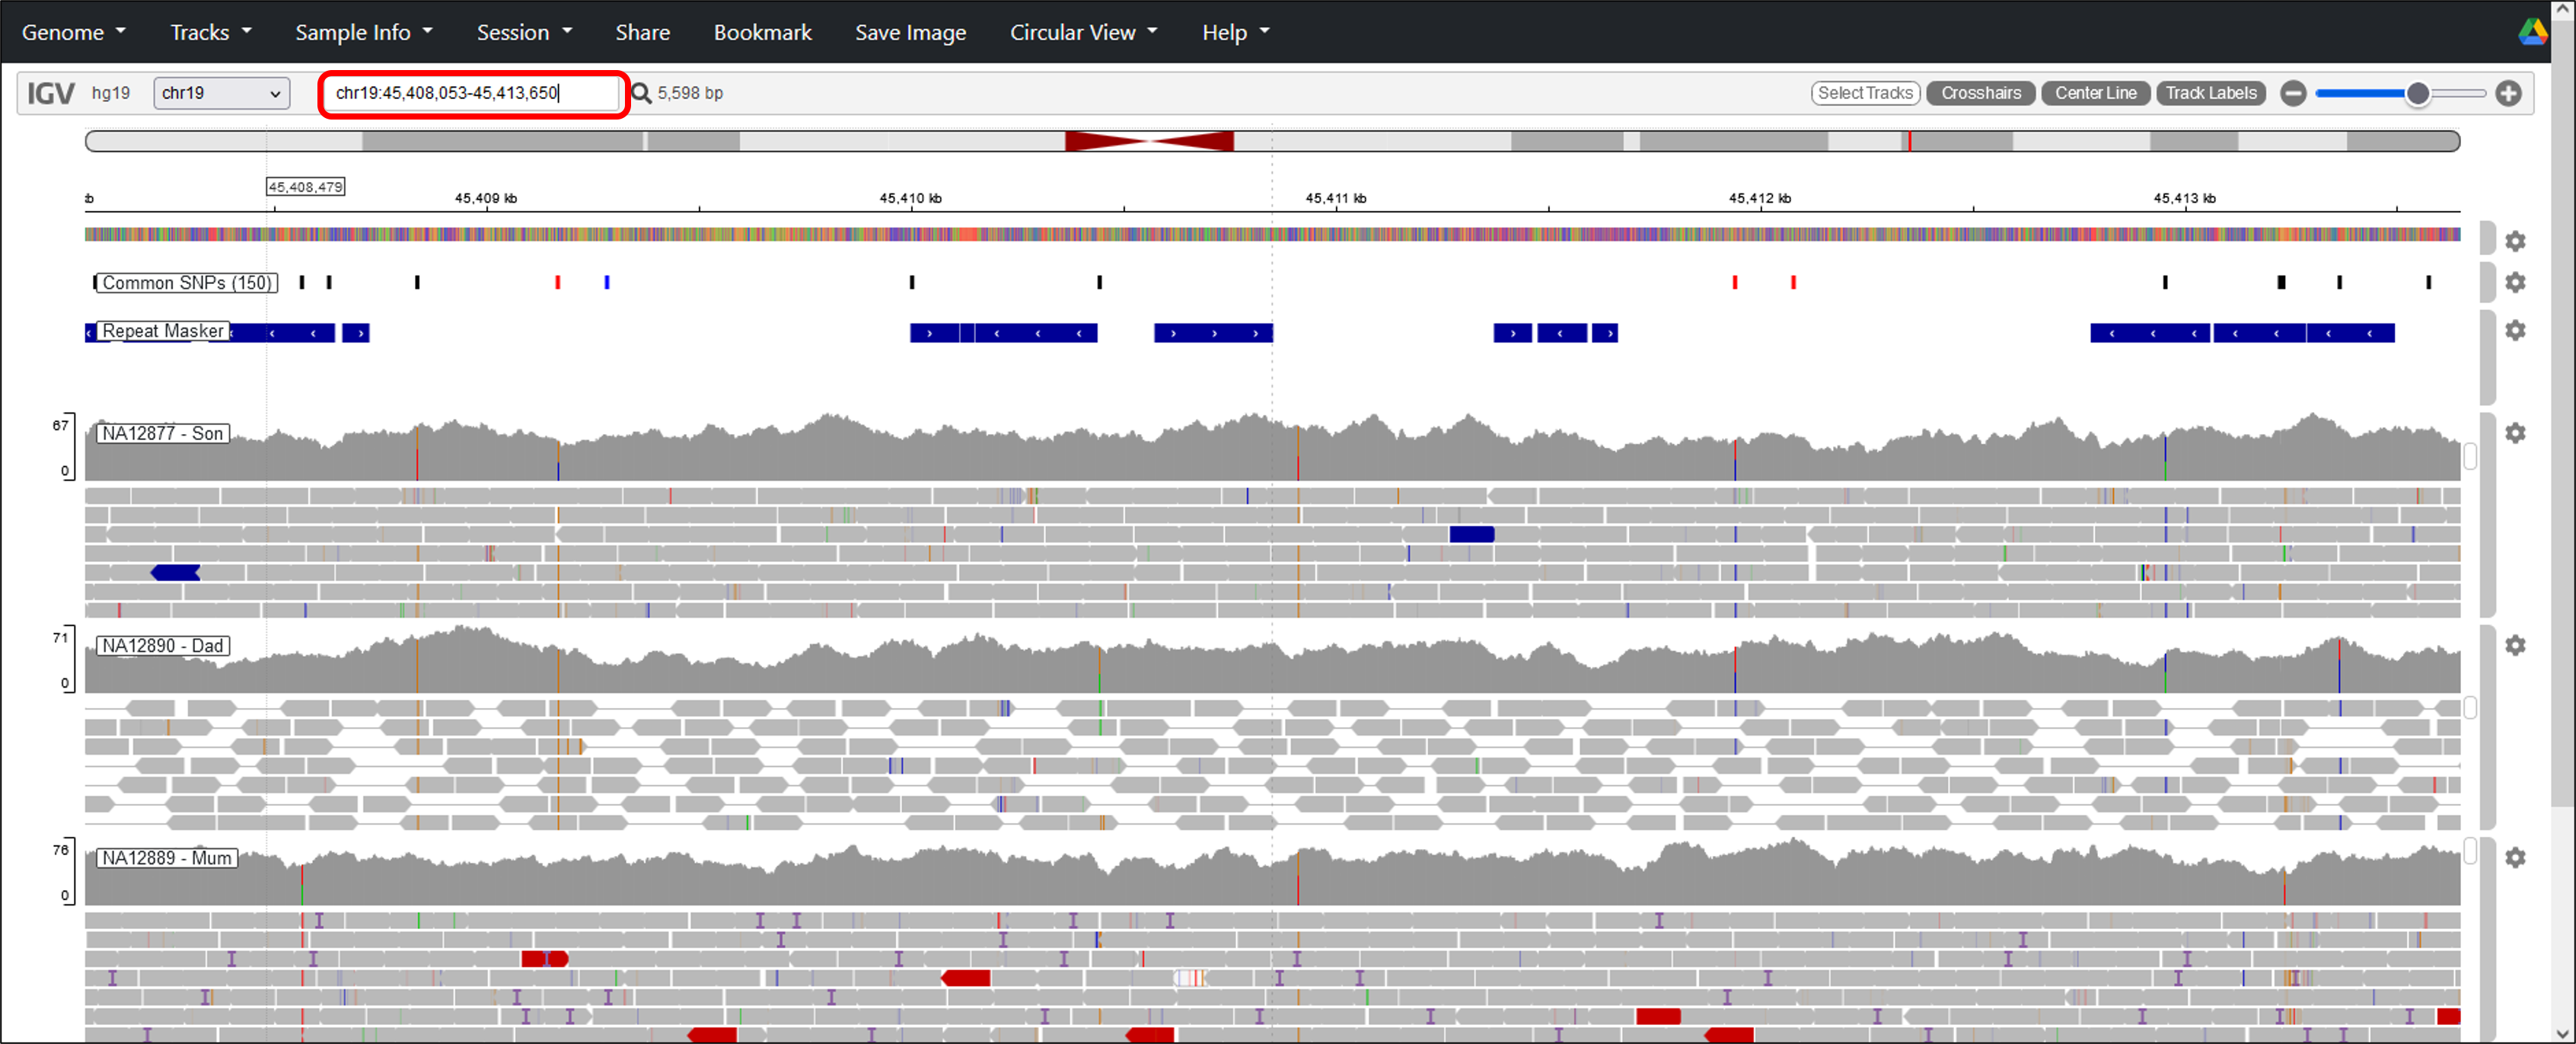
\includegraphics[keepaspectratio]{images/slide-51-image-1.png}}

Focus on the two common SNPs found in exon 4.

\pandocbounded{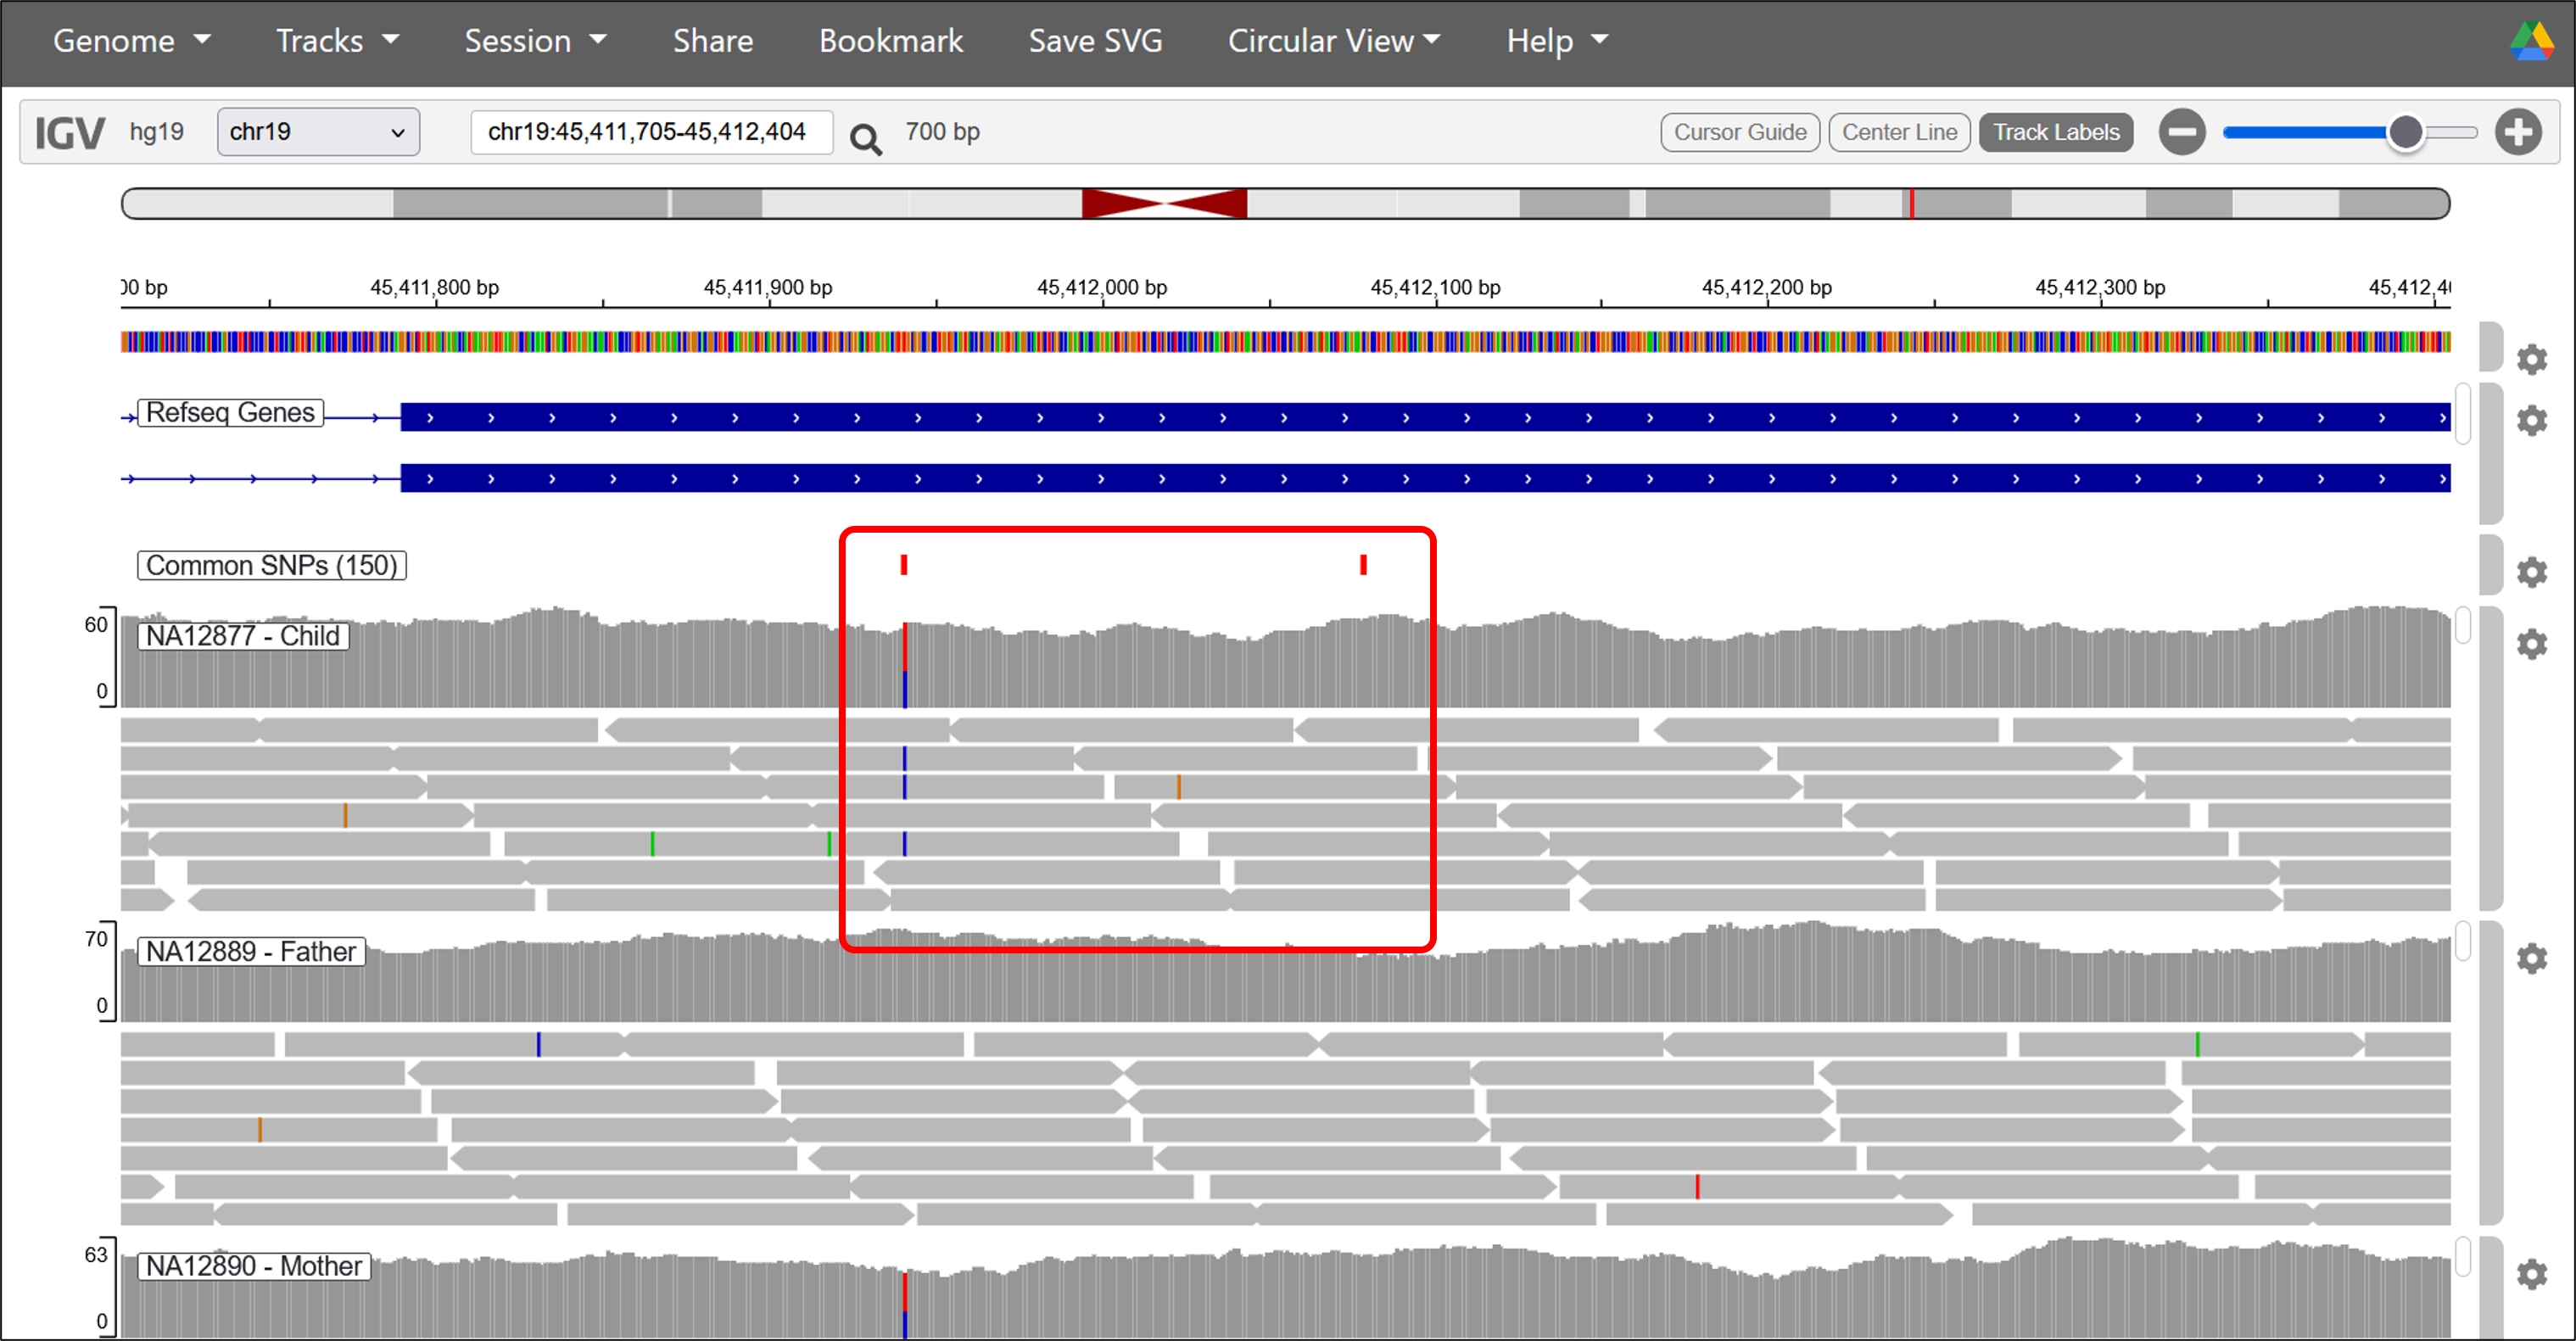
\includegraphics[keepaspectratio]{images/slide-52-image-1.png}}

Start with the variant at position chr19:45,411,941 (rs429358).

\pandocbounded{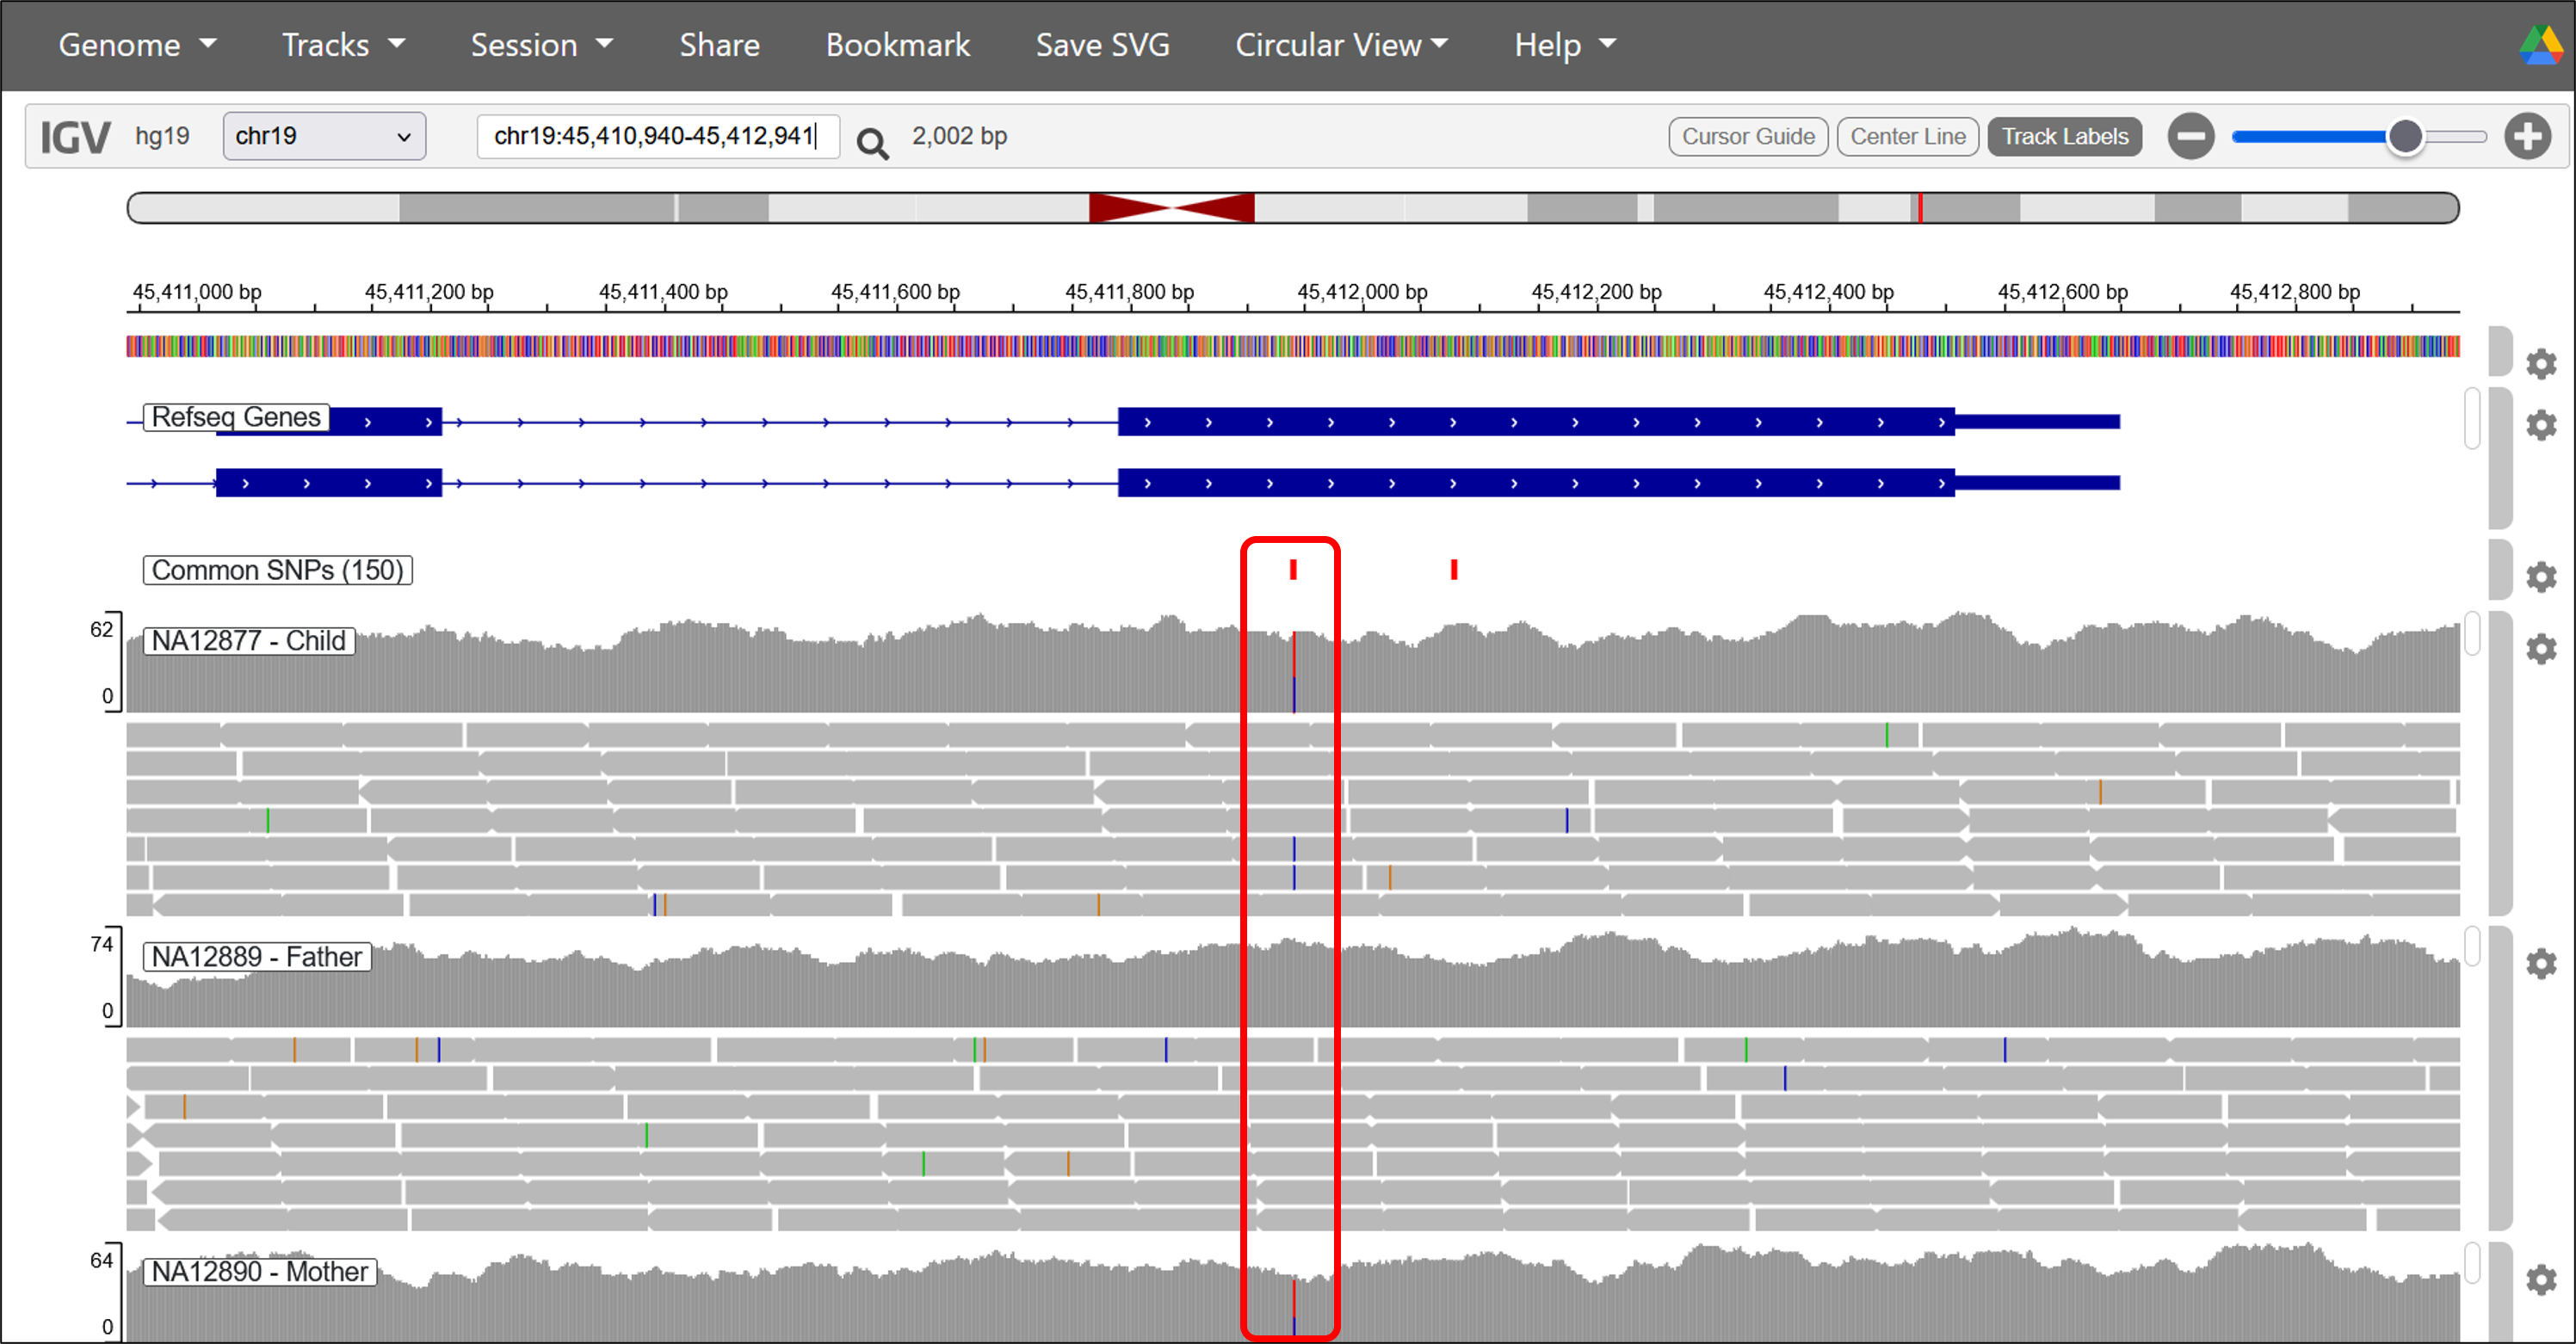
\includegraphics[keepaspectratio]{images/slide-53-image-1.png}}

\begin{quote}
\textbf{Test your understanding}

\begin{itemize}
\tightlist
\item
  What is the nature of the polymorphism at the DNA level?
\item
  Does this variant change the amino acid sequence? (You will have to
  turn on translation and work out which is the reading frame by looking
  at exon 1)
\item
  If so, from what to what?
\item
  What are the genotypes at this SNP for NA12877, NA12889 and NA12890?
\item
  What is the minor (alt) allele and the MAF?
\item
  What type of variant is this -- would it impact the protein?
\end{itemize}
\end{quote}

\begin{quote}
\textbf{Answer}

\begin{itemize}
\tightlist
\item
  The polymorphism at this site is C/T
\item
  Yes, this is a nonsynonymous mutation
\item
  The codon and amino acid changes from TGC (Cys) to CGC (Arg)
\item
  The genotypes are C/T for NA12877 (child), T/T for NA12889 (father)
  and C/T for NA12890 (mother)
\item
  The MAF for the minor (alt) C-allele is 18\%
\item
  This missense variant is protein altering. It is associated with
  predisposition to late-onset Alzheimer's disease (amongst other
  associations)
\end{itemize}
\end{quote}

We can use the \textbf{variant effect predictor (VEP)} tool to gain some
insight into potential functional effects of a given variant. Navigate
to the VEP site: \url{https://www.ensembl.org/tools/vep}

\begin{quote}
\textbf{Warning}

We will be using hg19/GRCh37 coordinates, so make sure you have the
right genome version selected.

\pandocbounded{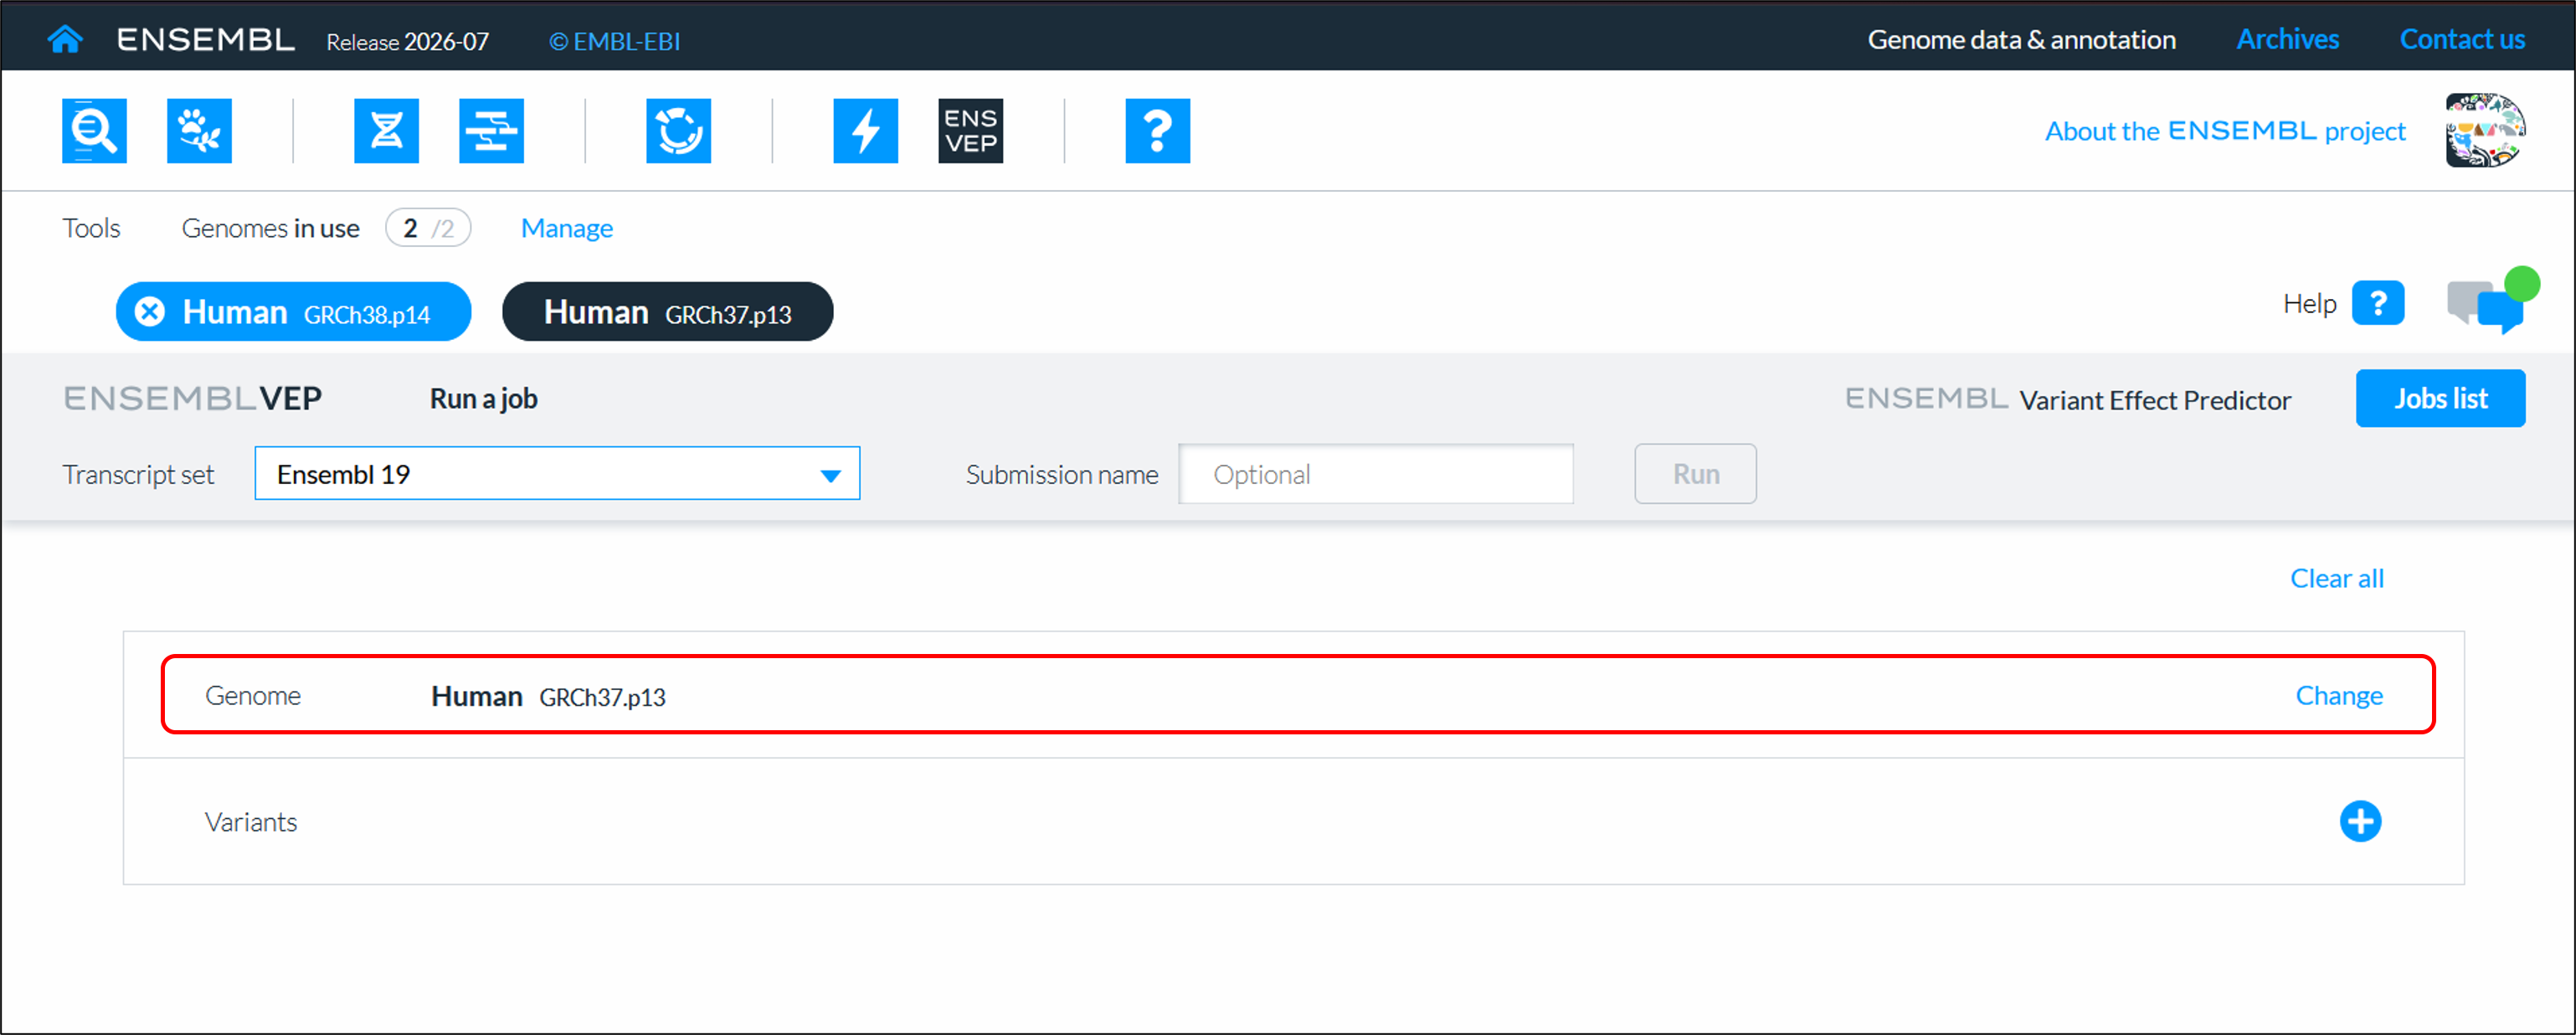
\includegraphics[keepaspectratio]{images/slide-53b-image-1.png}}
\end{quote}

A VEP search string has to be in a set format:

\begin{verbatim}
19 45411941 45411941 T C
\end{verbatim}

\begin{itemize}
\tightlist
\item
  The first number is the \textbf{Chromosome}
\item
  The second number is the start position
\item
  The third number is the end position (for a SNP, this is the same as
  the start position)
\item
  The fourth character is the wild-type base
\item
  The fifth character is the variant base(s) that the position will
  change to
\end{itemize}

Press ``Add'' when you've entered the details of the variant. Set the
\textbf{submission name} to something you will remember.

\pandocbounded{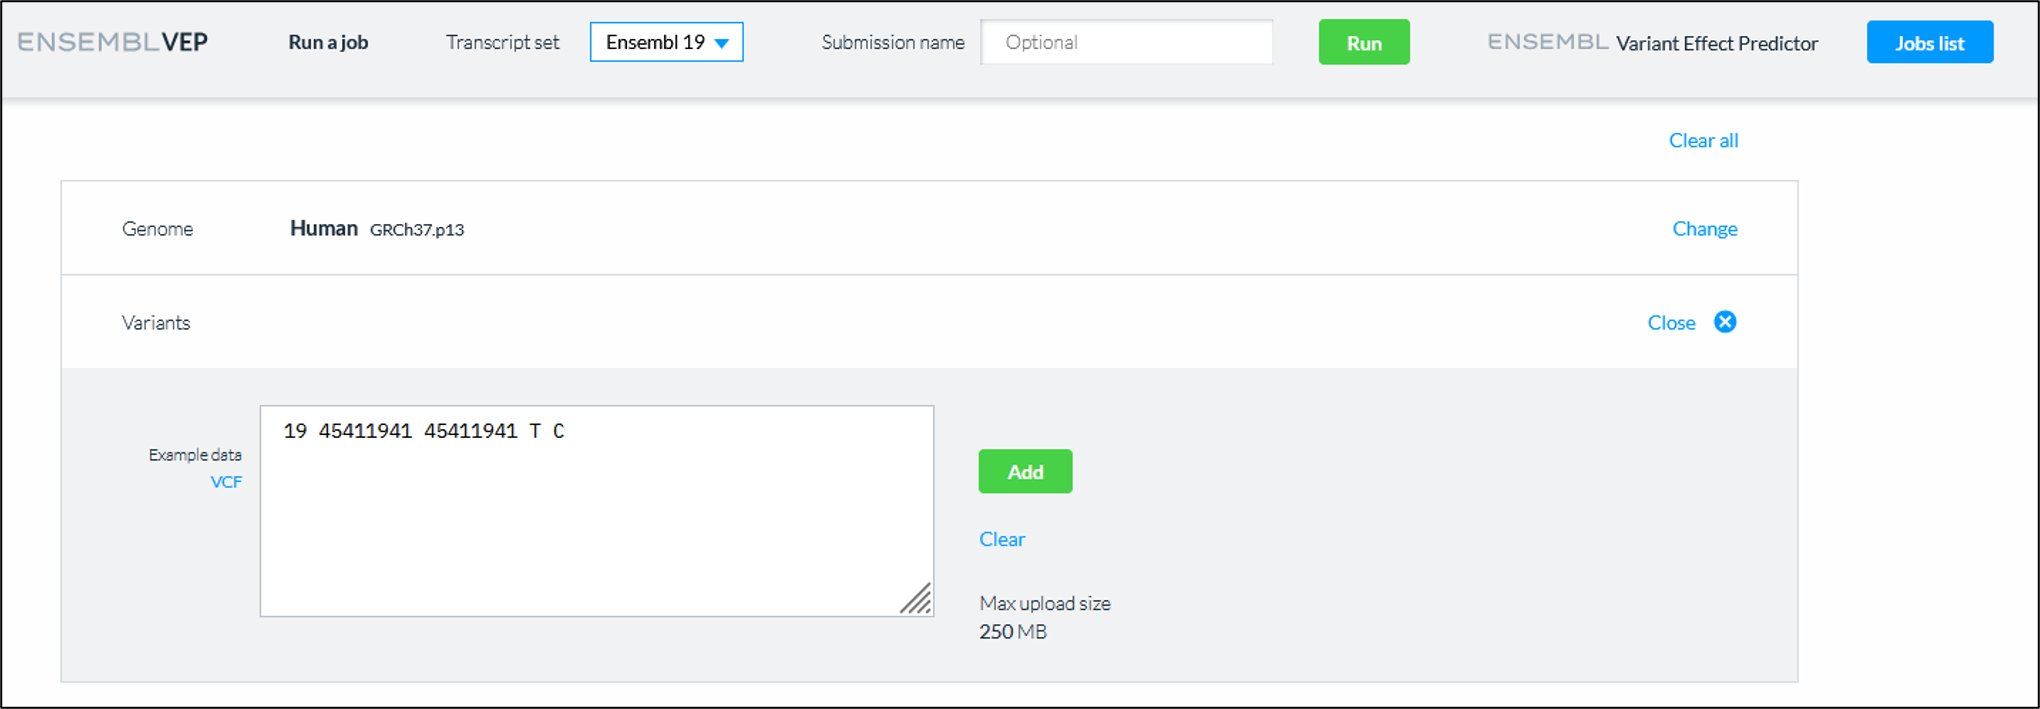
\includegraphics[keepaspectratio]{images/slide-54-image-1.png}}

We can also add some additional analyses to the job by scrolling down to
\textbf{Job Options}. For now, enable \textbf{REVEL} and \textbf{CADD}
under \textbf{Variant impact predictions}. These will help us predict
any effect that the variants might have.

\begin{quote}
\textbf{Tip}

\textbf{REVEL (Rare Exome Variant Ensemble Learner)} is a computational
tool that predicts whether a \textbf{missense} variant is likely to be
disease-causing by combining the results of multiple variant effect
prediction algorithms into a single score between 0 and 1. Higher REVEL
scores indicate a greater likelihood that the variant is pathogenic,
while lower scores suggest it is more likely to be benign. Although
there are no set thresholds, a general rule of thumb is:

\begin{itemize}
\tightlist
\item
  0.8+ : Pathogenic
\item
  0.5-0.8 : Likely Pathogenic
\item
  0.2-0.5 : Likely benign
\item
  \textless0.2 : Benign
\end{itemize}

(Ioannidis NM, Rothstein JH, Pejaver V, et al.~(2016) ``REVEL: An
Ensemble Method for Predicting the Pathogenicity of Rare Missense
Variants.'' \emph{American Journal of Human Genetics} 99(4):877-885.
\href{https://www.sciencedirect.com/science/article/pii/S0002929716303706?via\%3Dihub}{DOI:10.1016/j.ajhg.2016.08.016})

\textbf{CADD (Combined Annotation Dependent Depletion)} is a variant
prioritisation score that integrates multiple genomic annotations to
predict the deleteriousness of genetic variants. Higher CADD PHRED
scores indicate a greater likelihood of functional impact, with scores
above 20 typically considered potentially damaging.

CADD scores are ranked so that a score of 10 places a variant among the
top 10\% most deleterious variants in the genome, while a score of 20
places it among the top 1\%.

Although there are no set thresholds for CADD, a general rule of thumb
is:

\begin{itemize}
\tightlist
\item
  30+ : Deleterious
\item
  20-30 : Potentially deleterious
\item
  10-20 : Unlikely to be deleterious
\item
  \textless10 : Not deleterious
\end{itemize}

(Rentzsch P, Witten D, Cooper GM, Shendure J, Kircher M. (2019) ``CADD:
predicting the deleteriousness of variants throughout the human
genome.'' \emph{Nucleic Acids Research} 47(D1):D886-D894.
\href{https://academic.oup.com/nar/article/47/D1/D886/5146191}{DOI:10.1093/nar/gky1016})
\end{quote}

\begin{figure}[H]

{\centering \pandocbounded{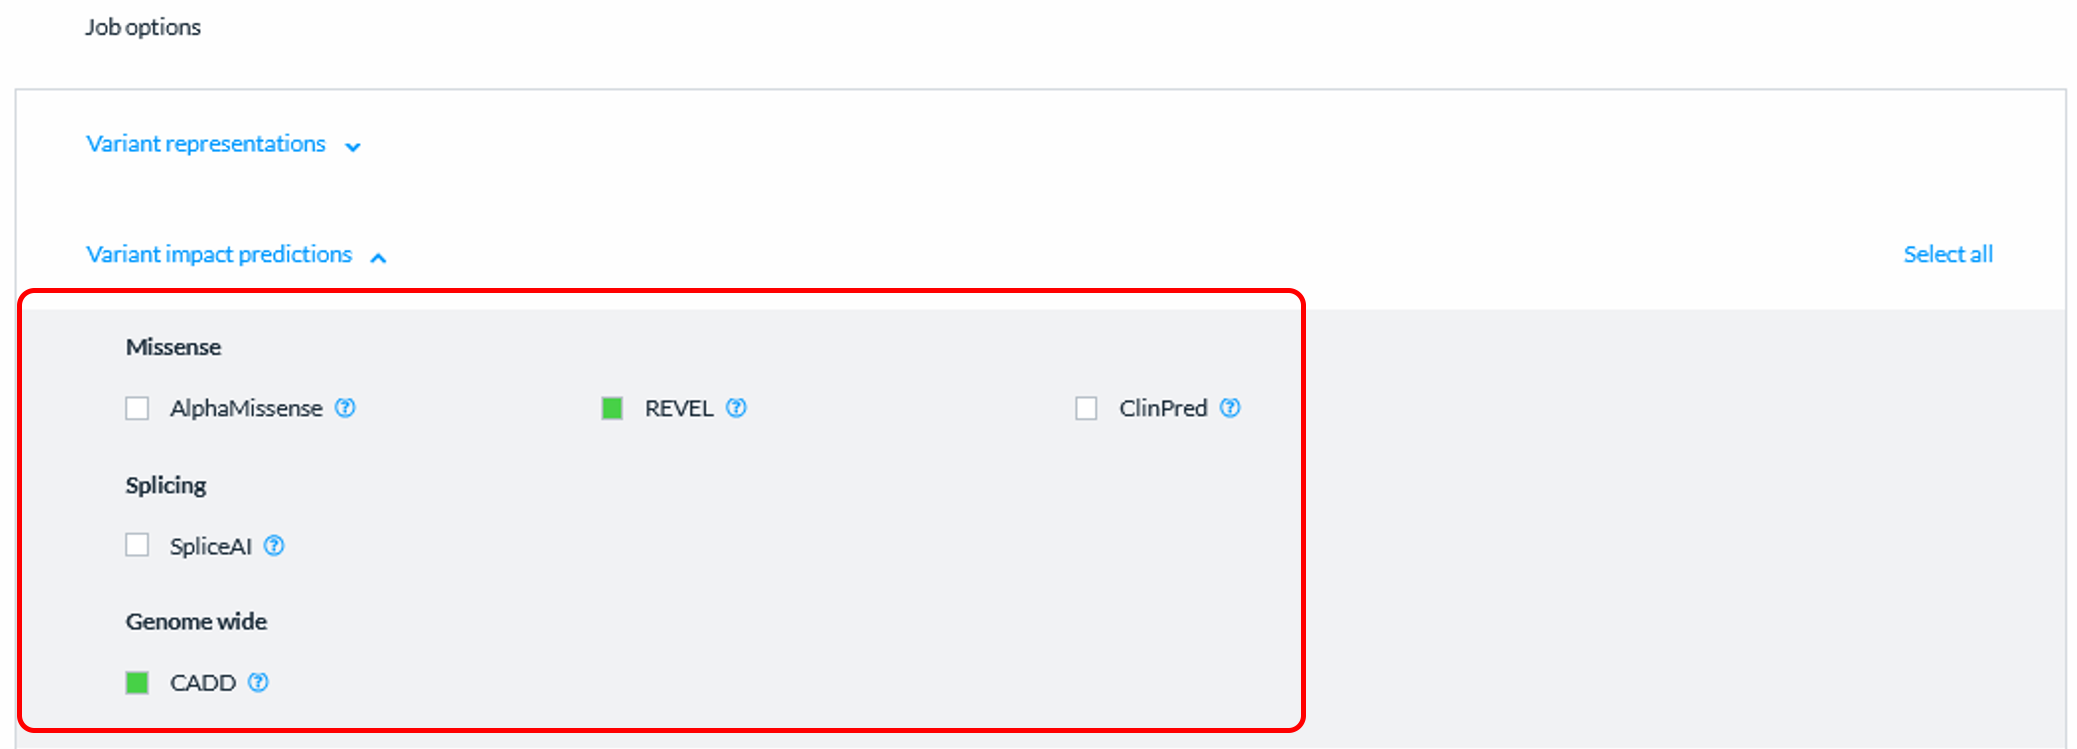
\includegraphics[keepaspectratio,alt={A screenshot demonstrating how to add REVEL and CADD information to a search in Ensembl VEP}]{images/slide-56-image-1.png}}

}

\caption{Screenshot from the original tutorial (slide 56).}

\end{figure}%

Press ``Run'' when you're ready. Your job will take a few minutes. Press
\textbf{Results} when it has finished.

\pandocbounded{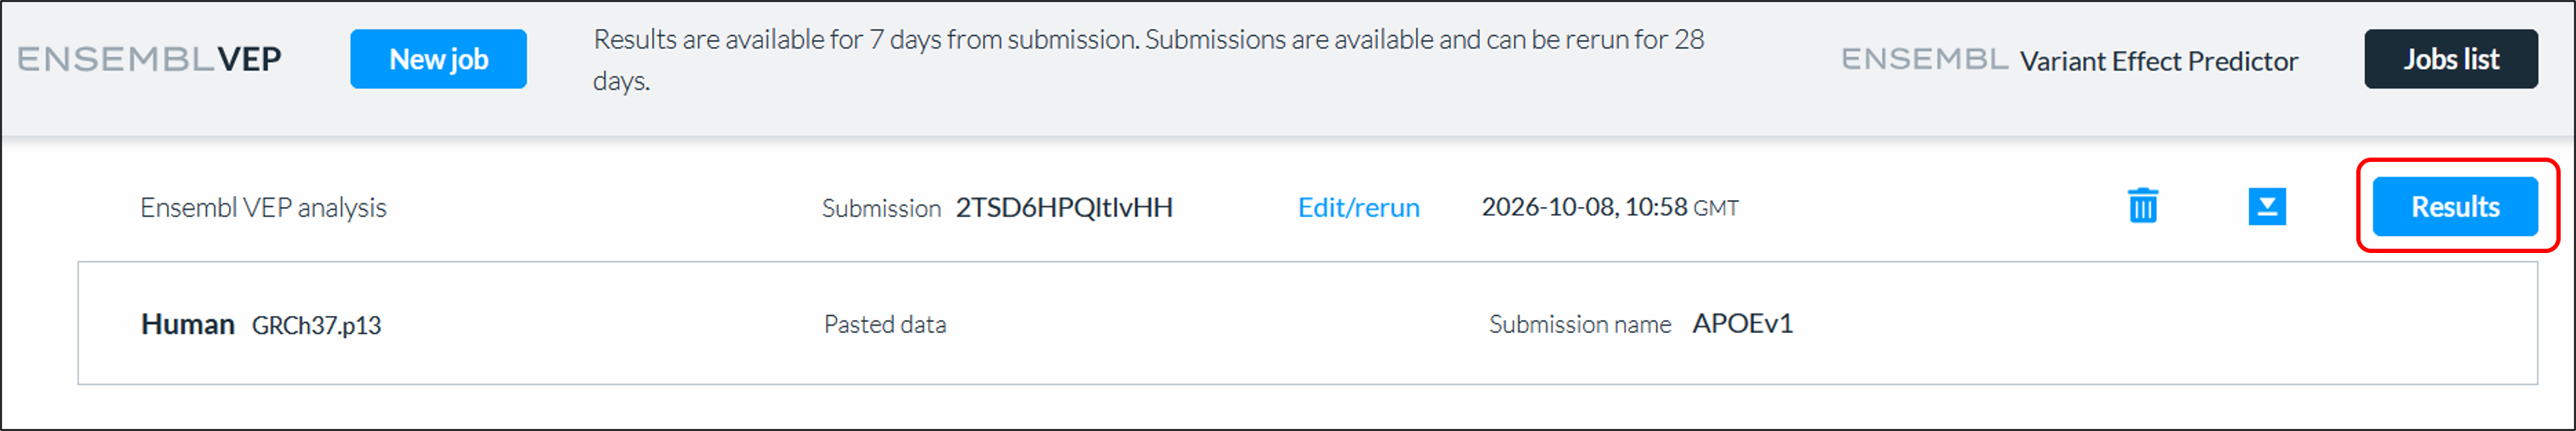
\includegraphics[keepaspectratio]{images/slide-57-image-1.png}}

\begin{quote}
\textbf{Test your understanding}

\begin{itemize}
\tightlist
\item
  What type of variant is this?
\item
  What might the REVEL score indicate about this variant? (You might
  have to click show annotations to see these details)
\item
  What might the CADD score indicate about this variant? (You might have
  to click show annotations to see these details)
\end{itemize}
\end{quote}

\begin{quote}
\textbf{Answer}

\begin{itemize}
\tightlist
\item
  This is a missense variant
\item
  A REVEL score of 0.229 is low and would generally be interpreted as
  evidence that the variant is likely benign (not disease-causing).
\item
  A CADD PHRED score of 13.75 suggests the variant is unlikely to be
  deleterious.
\end{itemize}

These low scores may partly reflect the high allele frequency of
approximately 15\%. The variant is unlikely to be associated with a
highly penetrant, early-onset condition. However, Alzheimer's disease is
common and usually develops after reproductive age.
\end{quote}

There is another SNP a bit further downstream (rs7412) we will examine
next.

\pandocbounded{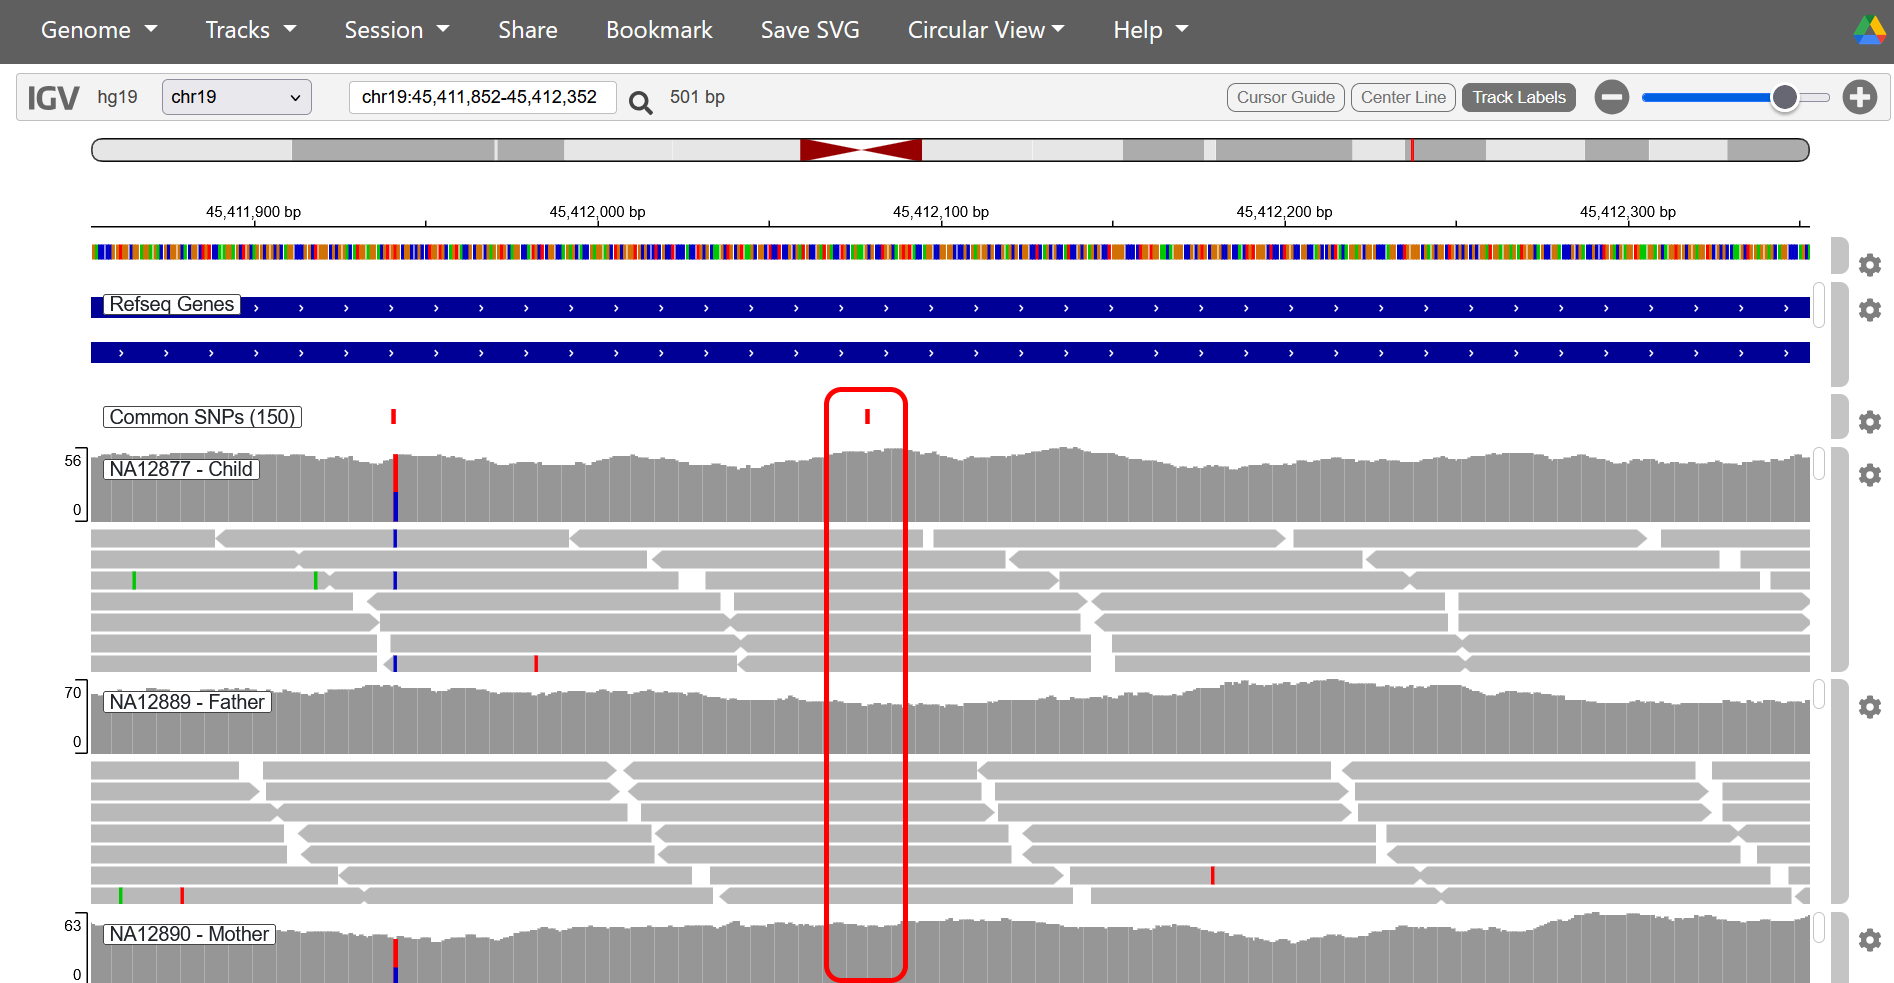
\includegraphics[keepaspectratio]{images/slide-58-image-1.png}}

\begin{quote}
\textbf{Test your understanding}

\begin{itemize}
\tightlist
\item
  What is the nature of the polymorphism at the DNA level?
\item
  Does this variant change the amino acid sequence?
\item
  If so, from what to what?
\item
  What are the genotypes at this SNP for NA12877, NA12889 and NA12890?
\item
  Is this variant likely to be pathogenic? (check using VEP)
\end{itemize}
\end{quote}

\begin{quote}
\textbf{Answer}

\begin{itemize}
\tightlist
\item
  The polymorphism is C/T
\item
  Yes, this is a nonsynonymous mutation
\item
  The codon and amino acid changes from CGC (Arg) to (TGC) Cys
\item
  The variant has a REVEL score of 0.588 and a CADD PHRED score of 25.8.
  This suggests it is more likely than the last variant to be pathogenic
  and potentially deleterious (use
  \texttt{19\ \ \ 45412079\ 45412079\ C\ T} to search)
\end{itemize}
\end{quote}

\bookmarksetup{startatroot}

\chapter{Case Study: Alzheimer's
disease}\label{case-study-alzheimers-disease}

Genetic, environmental and lifestyle factors contribute to late-onset
Alzheimer's disease (late-onset AD, LOAD), with genetic factors
contributing approximately 60\%. Variation at the \emph{APOE} gene locus
plays a contributory genetic role. \emph{APOE} encodes a very
low-density lipoprotein that helps remove cholesterol from the
bloodstream. The exact functional role of the protein encoded by
\emph{APOE} in LOAD remains unclear.

The major \emph{APOE} risk for LOAD is generally assumed to derive from
the ε2/ε3/ε4 haplotype system, with the e4 allele increasing risk for
the disorder and the e2 allele being protective. The ε2/ε3/ε4 haplotype
system is defined by the two non-synonymous SNPs in \emph{APOE} exon 4
that we just examined. One is a C/T SNP (rs429358) that encodes either
cysteine (C) or arginine (R) at amino acid 130. The second site defining
this haplotype system is a C/T SNP (rs7412), which again encodes
arginine (R) or cysteine (C) at amino acid 176.

The allelic compositions of the commonly investigated rs429358/rs7412
haplotypes are:

\begin{itemize}
\item
  T--T for ε2
\item
  T--C for ε3
\item
  C--C for ε4
\end{itemize}

{\def\LTcaptype{none} % do not increment counter
\begin{longtable}[]{@{}llll@{}}
\toprule\noalign{}
& rs429358 & rs7412 & Frequency and Prognosis \\
\midrule\noalign{}
\endhead
\bottomrule\noalign{}
\endlastfoot
\emph{APOE} ε2 & T & T & Rare, possibly protective \\
\emph{APOE} ε3 & T & C & Common, neutral \\
\emph{APOE} ε4 & C & C & 20\% frequency, risk variant \\
Not observed & C & T & \\
\end{longtable}
}

\begin{quote}
\textbf{Test your understanding}

\begin{itemize}
\tightlist
\item
  What are the \emph{APOE} exon 4 haplotypes for NA12877, NA12889 and
  NA12890 and their relative LOAD risk status?
\item
  Why might the C--T haplotype not be observed?
\end{itemize}
\end{quote}

\begin{quote}
\textbf{Answer}

The haplotypes and relative LOAD risk are:

\begin{itemize}
\tightlist
\item
  NA12877: T--T \emph{APOE} ε2 possibly protective, T--C \emph{APOE} ε3
  neutral
\item
  NA12889: T--T \emph{APOE} ε2 possibly protective, T--T \emph{APOE} ε2
  possibly protective
\item
  NA12890: T--T \emph{APOE} ε2 possibly protective, T--C \emph{APOE} ε3
  neutral
\end{itemize}

The C-T haplotype may not be observed, as the two variants are very
close and the probability of a recombination event generating the fourth
recombinant haplotype is very low
\end{quote}

\bookmarksetup{startatroot}

\chapter{Case Study: Zellweger
syndrome}\label{case-study-zellweger-syndrome}

A family is referred to clinical genetics with a severely ill newborn
child who has received a clinical diagnosis of probable Zellweger
syndrome. This is an autosomal recessive systemic disorder characterised
clinically by severe neurologic dysfunction, craniofacial abnormalities,
and liver dysfunction, and biochemically by the absence of peroxisomes.
Zellweger syndrome is characterised by locus heterogeneity and can be
caused by mutations in any one of several genes, encoding proteins known
as pexins, which are involved in peroxisome biogenesis. In order to try
and provide a genetic diagnosis, whole exome sequencing was performed in
the family and variants in a known Zellweger gene, \emph{PEX3},
detected:

{\def\LTcaptype{none} % do not increment counter
\begin{longtable}[]{@{}llccc@{}}
\toprule\noalign{}
Gene & Position (GRCh37/hg19) & Mother & Father & Affected child \\
\midrule\noalign{}
\endhead
\bottomrule\noalign{}
\endlastfoot
\emph{PEX3} & 6:143784092 & A/A & A/G & A/A \\
\emph{PEX3} & 6:143792714 & G/TG & G/G & G/TG \\
\emph{PEX3} & 6:143795928 & T/T & T/A & T/A \\
\emph{PEX3} & 6:143800237 & T/C & T/T & T/T \\
\end{longtable}
}

\begin{quote}
\textbf{Test your understanding}

\begin{itemize}
\tightlist
\item
  How would you format a VEP query for each variant?
\item
  What are the predicted effects of these variants?
\end{itemize}
\end{quote}

\begin{quote}
\textbf{Answer}

The VEP search strings and likely effects would be:

\begin{itemize}
\tightlist
\item
  \texttt{6\ 143784092\ 143784092\ A\ G} - missense (Q/R), likely benign
\item
  \texttt{6\ 143792714\ 143792714\ G\ TG} - frameshift, likely
  deleterious
\item
  \texttt{6\ 143795928\ 143795928\ T\ A} - stop-gained variant,
  predicted to be deleterious
\item
  \texttt{6\ 143800237\ 143800237\ T\ C} - benign
\end{itemize}
\end{quote}

You can investigate the variants further in
\href{https://gnomad.broadinstitute.org}{gnomAD}. Make sure to use the
gnomAD version 2.1.1 so that GRCh37/hg19 is used and matches the genome
coordinates you have been using in IGV. Complete the following table:

\begin{quote}
\textbf{Test your understanding}

Complete the table:

{\def\LTcaptype{none} % do not increment counter
\begin{longtable}[]{@{}
  >{\raggedright\arraybackslash}p{(\linewidth - 10\tabcolsep) * \real{0.0722}}
  >{\raggedright\arraybackslash}p{(\linewidth - 10\tabcolsep) * \real{0.1340}}
  >{\centering\arraybackslash}p{(\linewidth - 10\tabcolsep) * \real{0.1031}}
  >{\raggedright\arraybackslash}p{(\linewidth - 10\tabcolsep) * \real{0.1959}}
  >{\centering\arraybackslash}p{(\linewidth - 10\tabcolsep) * \real{0.2577}}
  >{\raggedleft\arraybackslash}p{(\linewidth - 10\tabcolsep) * \real{0.2371}}@{}}
\toprule\noalign{}
\begin{minipage}[b]{\linewidth}\raggedright
Gene
\end{minipage} & \begin{minipage}[b]{\linewidth}\raggedright
Position
\end{minipage} & \begin{minipage}[b]{\linewidth}\centering
Genotype
\end{minipage} & \begin{minipage}[b]{\linewidth}\raggedright
Observed
\end{minipage} & \begin{minipage}[b]{\linewidth}\centering
Global allele frequency
\end{minipage} & \begin{minipage}[b]{\linewidth}\raggedleft
Number of homozygotes
\end{minipage} \\
\midrule\noalign{}
\endhead
\bottomrule\noalign{}
\endlastfoot
\emph{PEX3} & 6:143784092 & & & & \\
\emph{PEX3} & 6:143792714 & & & & \\
\emph{PEX3} & 6:143795928 & & & & \\
\emph{PEX3} & 6:143800237 & & & & \\
\end{longtable}
}

How would you interpret these data in terms of providing a diagnosis and
future risk assessment to the family? (In answering this question,
remember that the impact of a variant on the gene product may or may not
correlate with the effect size in terms of downstream phenotype. You'll
therefore need to use all the evidence available to you to predict
whether variants you are seeing in the data might be causative of
Zellweger syndrome or not)
\end{quote}

\begin{quote}
\textbf{Answer}

{\def\LTcaptype{none} % do not increment counter
\begin{longtable}[]{@{}
  >{\raggedright\arraybackslash}p{(\linewidth - 10\tabcolsep) * \real{0.0722}}
  >{\raggedright\arraybackslash}p{(\linewidth - 10\tabcolsep) * \real{0.1340}}
  >{\centering\arraybackslash}p{(\linewidth - 10\tabcolsep) * \real{0.1031}}
  >{\raggedright\arraybackslash}p{(\linewidth - 10\tabcolsep) * \real{0.1959}}
  >{\centering\arraybackslash}p{(\linewidth - 10\tabcolsep) * \real{0.2577}}
  >{\raggedleft\arraybackslash}p{(\linewidth - 10\tabcolsep) * \real{0.2371}}@{}}
\toprule\noalign{}
\begin{minipage}[b]{\linewidth}\raggedright
Gene
\end{minipage} & \begin{minipage}[b]{\linewidth}\raggedright
Position
\end{minipage} & \begin{minipage}[b]{\linewidth}\centering
Genotype
\end{minipage} & \begin{minipage}[b]{\linewidth}\raggedright
Observed
\end{minipage} & \begin{minipage}[b]{\linewidth}\centering
Global allele frequency
\end{minipage} & \begin{minipage}[b]{\linewidth}\raggedleft
Number of homozygotes
\end{minipage} \\
\midrule\noalign{}
\endhead
\bottomrule\noalign{}
\endlastfoot
\emph{PEX3} & 6:143784092 & A/G & yes (rs35220041) & 0.02818 & 615 \\
\emph{PEX3} & 6:143792714 & G/TG & no & N/A
(\textless1/\textasciitilde282,000) & 0 \\
\emph{PEX3} & 6:143795928 & T/A & no & N/A
(\textless1/\textasciitilde251,000) & 0 \\
\emph{PEX3} & 6:143800237 & T/C & no & N/A
(\textless1/\textasciitilde251,000) & 0 \\
\end{longtable}
}

The data strongly support a diagnosis of Zellweger syndrome in the
affected child, who is compound heterozygous for two predicted
high-impact PEX3 variants, one frameshift and one premature stop
variant, neither of which has been observed in gnomAD. Although the
impact of the 143784092 variant is predicted as moderate, this allele is
relatively frequent (\textasciitilde2\% globally and 17\% in the
Latino/admixed American population), and at least 600 homozygotes have
been observed, so it is unlikely to be a disease allele. The 143800237
variant is novel, but synonymous, so it is again unlikely to be
pathogenic. Thus, each parent carries a different candidate pathogenic
allele. The recurrence risk is 25\% for each pregnancy, assuming the
variants are confirmed to be in trans and causative.
\end{quote}

\bookmarksetup{startatroot}

\chapter{References and useful links}\label{references-and-useful-links}

\begin{itemize}
\tightlist
\item
  Eberle MA et al.~(2017). A reference data set of 5.4 million phased
  human variants validated by genetic inheritance from sequencing a
  three-generation 17-member pedigree. \emph{Genome Research}
  27:157--164. \url{https://doi.org/10.1101/gr.210500.116}
\item
  IGV web application: \url{https://smb-informatics.mvls.gla.ac.uk/igv}
\item
  University VPN: \url{https://www.gla.ac.uk/myglasgow/it/vpn/}
\item
  Ensembl: \url{https://www.ensembl.org/}
\item
  Ensembl VEP: \url{https://www.ensembl.org/tools/vep}
\item
  gnomAD: \url{https://gnomad.broadinstitute.org/}
\end{itemize}

\end{tcolorbox}




\end{document}
